%Präambel%
\documentclass[9pt, openright=false]{scrartcl}
%\usepackage[onehalfspacing]{setspace} %
\usepackage[ngerman]{babel}
\usepackage[utf8]{inputenc}
\usepackage{sanitize-umlaut}
\usepackage{graphicx}
\usepackage{amsmath}
\usepackage{amssymb}
\usepackage{multicol}
\usepackage{helvet}
\usepackage{lastpage}
\usepackage{geometry}
\usepackage{colortbl}
\usepackage{multirow}
\usepackage{wrapfig}
\usepackage{imakeidx}
\makeindex[options=-g -s index.ist]
\renewcommand{\familydefault}{\sfdefault}
%Kopfzeile%
\usepackage[headsepline, footsepline]{scrlayer-scrpage}
\pagestyle{scrheadings}
\clearpairofpagestyles
\setkomafont{pageheadfoot}{\normalfont\small}
\ihead{
\includegraphics[height=45pt]{images/HSRLOGO.jpg}}
\chead{}
\ohead{Zusammenfassung \\ Siedlungswasserwirtschaft 3}
\ifoot{Züger B16}
\cfoot{}
\ofoot{\pagemark /\pageref{LastPage}}
%Seitengeometrie festlegen%
\geometry{left=30mm, right=20mm, top=38mm, bottom=20mm, includefoot=false, headsep = \dimexpr2\baselineskip\relax, footskip = \dimexpr1\baselineskip+3.5mm\relax,}
%Fusszeitenlinie höher setzen%
\ModifyLayer[addvoffset=-.8ex]{scrheadings.foot.above.line}
\ModifyLayer[addvoffset=-.8ex]{plain.scrheadings.foot.above.line}
\setcounter{tocdepth}{3}
\usepackage{booktabs}			% Schönere Tabellen
\usepackage{tabularx}			% Tabellen auf Seitenbreite
\usepackage{enumitem} 
\newlist{citemize}{itemize}{4} 
\setlist[citemize]{label=\textbullet ,nosep,topsep=-\parskip} 
%Tabellen///////////////////////////////////////////////////%
\newcolumntype{L}[1]{>{\raggedright\arraybackslash}p{#1}} % Tabelleninhalt linksausgerichtet
\newcolumntype{R}[1]{>{\raggedleft\arraybackslash}p{#1}} % Tabelleninhalt rechtsausgerichtet
\newcolumntype{C}[1]{>{\centering\arraybackslash}p{#1}} %  Tabelleninhalt zentriert
\usepackage{titlesec}
\newcommand{\sectionbreak}{\clearpage}

\begin{document}
%//////////////////////////////////////%
%//////////////////////////////////////%
%Titelseite%
%//////////////////////////////////////%
\begin{titlepage} 
\vspace*{-\topskip}\vspace*{-\headsep} \vspace{-1.4cm}


\includegraphics[height=45pt]{images/HSRLOGO.jpg} 

\vspace{\headsep}\vspace{\topskip}
   \centering 
   \vspace{3cm}
   \fontsize{30pt}{13pt}\selectfont Zusammenfassung \\ \vspace{1cm} Siedlungswasserwirtschaft 3\\ 
   \vspace{1ex} 
   
   \vspace{1cm} 
   \Large  
   \today \\ 
   Züger Raphael \\
   \vspace{1cm} 
  \normalsize
  Diese Zusammenfassung wurde mit Hilfe von {\LaTeX} gesetzt.\\ \vspace{1cm}
   \large 
   \normalsize 
   Quellen: Vorlesungen von Prof. Dr. Michael Burkhardt
   
   
   \clearpage
   \tableofcontents
\end{titlepage} 
\pagebreak

\section{Einführung Wasser}
\index{Wasserverteilung}Wasserverteilung auf der Erde: 3\% \index{Wasserverteilung!Süsswasser}Süsswasser, weniger als 1\% \index{Wasserverteilung!Grundwasser}Grundwasser und 0.3\% \index{Wasserverteilung!Oberflächenwasser}Oberflächenwasser, 97\% des Wassers auf der Erde ist \index{Wasserverteilung!Salzwasser}Salzwasser (Ozeane). Der Wasserbedarf steigt massiv an. Heute macht die
\begin{wrapfigure}{l}{8cm} 
  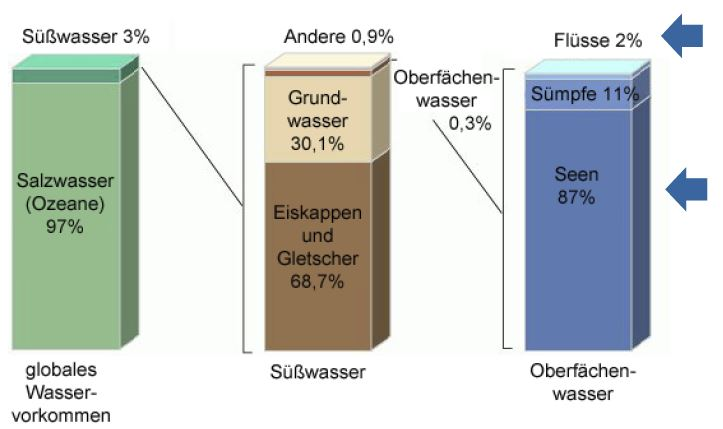
\includegraphics[width=.5\textwidth]{images/wasservetreilung}
\end{wrapfigure} Landwirtschaft rund 70\% des weltweiten \index{Wasserverbrauch}Wasserverbrauchs aus. Gleichzeitig wird 30\% der weltweiten Gesamtenergie für die Nahrungsmittelerzeugung und ihre Versorgungskette aufgewendet.\\ \\
Der weltweite Wasserverbrauch pro Kopf und Tag ist sehr unterschiedlich. In Indien beträgt er gerade mal 25 Liter pro Kopf und Tag. In Dubai hingegen 500 Liter pro Kopf und Tag. Die Bevölkerung in Dubai kann sich das nur leisten, weil die Entsalzungsanlagen vom Staat subventioniert werden. Ansonsten wäre Wasser in der Wüste unbezahlbar. Weltweit haben 800 Millionen Menschen keinen Zugang zu sauberem Trinkwasser. 2.6 Milliarden Menschen (40\%) haben keinen Zugang zu sicheren sanitären Systemen und rund 1 Milliarde Menschen verrichten ihre Notdurft draussen. Vor allem der nahe und mittlere Osten, Ostasien, der pazifische Raum und Afrika sind betroffen.\\ \\
2030 werden 47\% der Menschheit in Wassermangel-Gebieten leben und das \index{Wasserdefizit}Wasserdefizit wird auf über 30\% steigen. Der Wasserverbrauch nimmt dabei überproportional zum Bevölkerungswachstum zu. Gleichzeitig steigt der Bevölkerungsanteil, welcher in einer Stadt lebt, was sowohl die Wasserver- und Entsorgung vor neue Herausforderungen stellt. Man geht davon aus, dass bereits 2050 rund 70\% der Weltbevölkerung in städtischen Gebieten leben werden. Heutige Probleme in Bezug zur Wasserver- und Entsorgung:
\begin{itemize}
\item Versiegelung und Wasserverschmutzung
\item Begrenzter Zugang zu Wasser und hohe Mobilität
\end{itemize}
Die \index{Wasserressourcen}Wasserressourcen werden knapp (Quantität) - Die Verfügbarkeit und Verteilung von Wasser ist unabhängig von den Voraussetzungen zu gewährleisten. Die kann zum Beispiel durch folgende Massnahmen erreicht werden:
\begin{itemize}
\item Zentrale Netze ausbauen / Dezentrale Systeme aufbauen
\item Solare Meer-, Brackwasserentsalzung; Zero-Discharge Industrien etc.
\end{itemize}
Die Wasserressourcen werden verschmutzt (Qualität) - Stoffeinträge verschmutzen die Wasserressourcen:
\begin{itemize}
\item Zukunftsfähigkeit von Wirtschaft und Gesellschaft bedroht sind (Pestizide, Metalle, Bakterien, etc.)
\item Verschmutzungen an der Quelle (source control) und nachgeschaltet (end-of-pipe)
entgegenwirken
\end{itemize}
Um auch in Zukunft diesen Problemen Herr zu werden, braucht es Innovative Konzepte: \\
Sichern von \index{Wasserressourcen}Wasserressourcen: Sicherung von Freiflächen, Grünflächen, Begrünung\\
Reinigen von verschmutztem Abwasser: Vierte Reinigungsstufe, Membrantechnik, zero-liquid-discharge\\
Schliessen des urbanen Wasserkreislaufs: Regenwasserspeicherung,-nutzung, Versickerung
\subsection{Beispiel Singapur}
Singapur hat einen jährlichen Niederschlag von 2'300 mm. Im Vergleich kommt Zürich nur auf 1'100 mm pro Jahr. Singapur hat ein drei Säulen System eingeführt um die Wasserversorgung sicher zu stellen:
\begin{itemize}
\item Regenwasser (stormwater; Bassins, Marina Bay)
\item Abwasser (wastewater; \glqq new water\grqq (Qualität von Trinkwasser))
\item Meerwasser (desaltination)
\end{itemize}
Die Stadt sammelt Brackwasser in riesigen Becken. Der Salzgehalt ist im Brackwasser geringer als in Meerwasser und die Entsalzung ist dadurch billiger. Gleichzeitig wird unterirdisch (bis 70m tief) das Abwasser der Stadt wieder aufbereitet und in Trinkwasserqualität in das Wasserversorgungsnetz eingeleitet.
\section{Entwicklung der Siedlungsentwässerung}
\subsection{Historische Entwicklung}
\paragraph{\index{Antike}Antike - Hoch entwickelte Leitungstechnik} Die Wasserleitungstechnik gelangte unter römischer Herrschaft zwischen dem ersten und fünften Jahrhundert in die Schweiz. Die Feinverteilung zu Gebäuden und zu \index{Laufbrunnen}Laufbrunnen wurde mit Rohrleitungen aus Blei, Holz oder Ton erstellt. Dabei handelte es sich bereits um Druckleitungen, welche vermutlich jeweils von einem Wasserturm gespiesen wurden. Auch im Bereich der Abwassertechnik waren die Römer Vorreiter. In Avenches, Augusta Raurica und Windonissa sind heute noch antike Wasser- und Abwasserleitungen sichtbar. Meist sind jedoch nur Kalksinterstränge als Überreste von Teucheln (ausgebohrte Baumstämme) erhalten geblieben.\\
In Vindonissa wurden so 1.3 Millionen Liter Frischwasser zur Versorgung von 6000 Legionären in die Stadt gebracht. Die Zuleitungen hatten nur ein Gefälle von 4 mm/m. Das Schmutzwasser wurde im Abwasserkanal (cloaca maxima) in die Aare geleitet.
\paragraph{\index{Mittelalter}Mittelalter - Abwasserentsorgung durch Flüsse} Im Mittelalter ging das Wissen der Antike verloren und es grassierten viele Seuchen. In den Städten stützte sich die \index{Wassergewinnung}Wassergewinnung auf Grundwasser. Ein Beispiel ist der Amazonenbrunnen in Zürich, welcher seit 1430 aktenkundig ist und Quellwasser liefert. In Städten nahe am Wasser wurde auch das Oberflächenwasser genutzt. Dazu wurden Schöpfräder und Pumpwerke gebaut. Die Leitungen bestanden hauptsächlich aus \index{Teucheln}Teucheln, welche oberirdisch verlegt wurden. Als Kanalisation wurden die Stadtbäche eingesetzt.\\ \\ Durch die Vernetzung innerhalb der Stadt verbreiteten sich Keime sehr schnell. So wurden viele \index{Epidemien}Epidemien ausgelöst. Vor allem im 19. Jahrhundert traten in europäischen Städten viele katastrophale Epidemien auf. Dabei starben bis zu 50\% der erkrankten Menschen. Ein Beispiel ist die \index{Typhusepidemie}Typhusepidemie 1884 in Zürich, bei welcher 1600 Menschen erkrankten. Als erste Massnahme wurde das Trinkwasser abgekocht. Bis zur Entdeckung der Krankheitserreger \index{Cholera}Cholera (1883) und \index{Typhus}Typhus (1906) galt Trinkwasser als \glqq ungefährlich\grqq . Als Reaktion darauf wurde die Schwemmkanalisation und Sandfiltration aus England eingeführt.
\paragraph{Heute - Aufgaben erfüllen mit technischer Infrastruktur} Heute ist die Abwasserentsorgung komplett von der Wasserversorgung getrennt. Es bestehen somit zwei komplett getrennte Infrastrukturen. Unerwünschte Schmutzstoffe werden aus dem Abwasser entfernt. Anfallende Schlämme werden aufbereitet und entsorgt. Die Entsorgung ist damit zuverlässig und ökonomisch.\\
\begin{center}
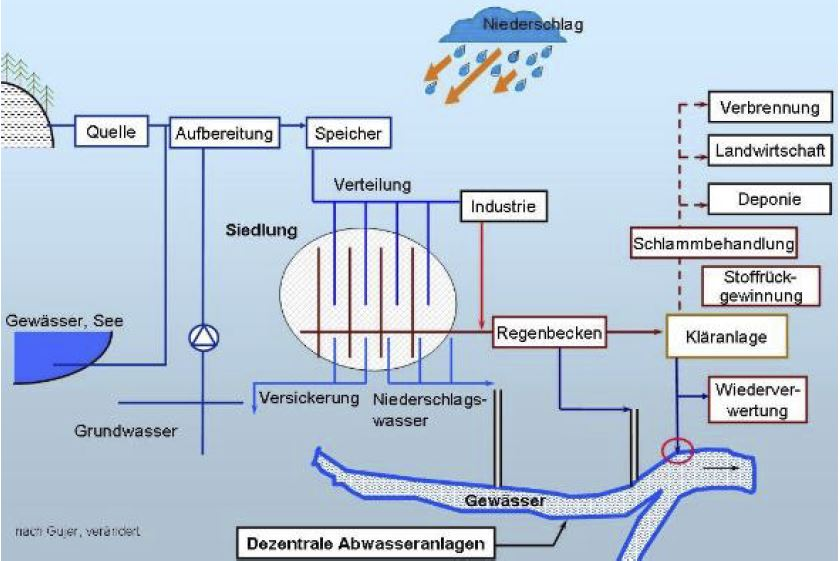
\includegraphics[width=.6\textwidth]{images/netze}
\end{center}
\subsection{Grundlagen Schweizer Siedlungsentwässerung} 
In der Schweiz wird Schmutz- und Regenwasser über ein\index{Kanalnetz} Kanalnetz mit einer Länge von über 47'000 km abgeleitet. Es handelt sich dabei um eine Schwemmkanalisation mit mittleren Gefällen zwischen 0.5\% und 5\%. Rund zwei drittel des Netzes wurden in den letzten 50 Jahren erbaut und der \index{Wiederbeschaffungswert}Wiederbeschaffungswert beträgt zirka 55 Milliarden Franken. Das Abwasser wird in 750 zentralen Kläranlagen ($>$ 500 EW Grösse) mit einem Wiederbeschaffungswert von zirka 10 Milliarden Franken und 3'400 Kleinkläranlagen im suburbanen und ländlichen Raum gereinigt. Die Abwasserinfrastruktur ist öffentliches Eigentum und gehört den Gemeinden oder Städten. \clearpage
Von den entwässerten Flächen gehören 50\% (100'000 ha) zu Gemeinden mit rund 20\% der Gesamtbevölkerung. Die \index{Kleinteiligkeit}Kleinteiligkeit beeinflusst dabei den Netzunterhalt, Abwassergebühren, bauliche und technologische Weiterentwicklung. Der Anschlussgrad an eine Kläranlage stieg von 14\% (1965) auf 97.7\% (2011). Ein weiteres Prozent könnte angeschlossen werden. Bei den restlichen Prozent ist ein Anschluss nicht sinnvoll, da diese in abgelegenen oder schwach besiedelten Gebieten leben. Bei diesen Landet das Abwasser meistens in einer Grube.\\ \\
Das gereinigte Abwasser wird in Oberflächengewässer eingeleitet. Dazu müssen die Einleitbedingungen gemäss Gewässerschutzverordnung (GSchV) beachtet werden. Die dort festgelegten Grenzwerte müssen zwingend eingehalten werden. Neben der Einleitung in ein Oberflächengewässer gibt es auch andere Möglichkeiten, welche bei uns jedoch nicht eingesetzt werden:
\begin{itemize}
\item Vollständiges Recykling
\item Einleitung in Grundwasser
\item Verdampfen (Eindampfen)
\end{itemize}
\subsection{Trenn- und Mischsystem}
\paragraph{Mischkanalisation (GSchG 1971)} Die Siedlungsentwässerung soll Abwasser ableiten und in geeigneter Form und mit geeigneter Qualität einer Vorflut zuleiten. Nach dieser \glqq Ingenieur-Philosophie\grqq wurden Kanalisationen in den 70er Jahren gebaut. Dazu wurden für die Ableitung und Reinigung von Abwässer die erforderlichen öffentlichen Kanalisationssysteme und zentralen ARA's gebaut (zentrale Netzinfrastruktur). Der Bau der Kanalisationen stützte sich auf generelle Projekte, welche der zu erwartenden baulichen Entwicklung Rechnung tragen sollten. Bis 1991 wurden alle Abwasserarten zusammen gefasst und zur Kläranlage geleitet. Dieses traditionelle Schweizer System hat einen Verbreitungsgrad von rund 70 \%. In den Gebäuden wurde jedoch schon damals ein zwei Rohr System gebaut. Da in der Mischkanalisation auch Regenwasser abgeleitet wird, kommt es auch immer wieder bei Regen zu diversen Problemen. Das stark schwankende Wasserregime im Abwassernetz führt zu:
\begin{itemize}
\item Hydraulische Überlastung der Kläranlagen, dadurch häufiges Anspringen von Mischwasserentlastungen
\item Verminderter Wirkungsgrad der Kläranlagen durch Verdünnung des verschmutzten Abwassers, dadurch teils Überdimensionierung von Kläranlagen (Platz-/Kostenfrage)
\item Direkteintrag von Schmutzstoffen unter Umgehung der Kläranlage ins Gewässer
\item Bauliche Entwicklung mit versiegelten Flächen kaum vorhersehbar (immer mehr)
\end{itemize}
\paragraph{Trennkanalisation (seit GSchG 1991)} In der Trennkanalisation wird Niederschlagswasser getrennt gefasst und entsorgt. Dieses System weist einen Verbreitungsgrad von rund 30\% auf. Im Gebäude wird ein drei Rohr System gebaut. In Neubaugebieten ist die Verbreitung deutlich höher. Das verschmutzte Regenabwasser muss erst behandelt, dann versickert oder in ein Gewässer geleitet werden und darf nur im letzten Fall in die Kläranlage geleitet\begin{wrapfigure}{r}{8cm} 
  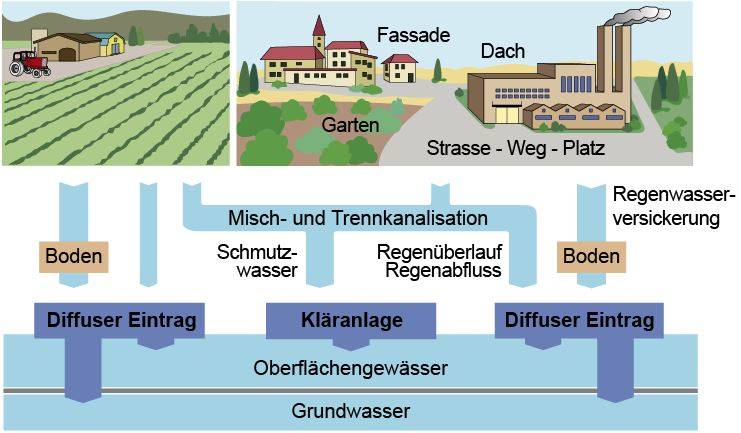
\includegraphics[width=.5\textwidth]{images/uebersicht}
\end{wrapfigure} werden. Durch die getrennte Entsorgung von verschmutztem und nicht verschmutztem Abwasser wird eine Verunreinigung des Bodens und der Gewässer verhindert. Weiter wird dadurch eine hohe Rohwasserqualität für das Trinkwasser sichergestellt. Das verschmutzte Abwasser muss behandelt werden und darf nur mit einer kantonalen Bewilligung in ein Gewässer eingeleitet oder versickert werden. Es besteht ein Behandlungsgebot beziehungsweise ein Versickerungsverbot für unbehandeltes Wasser. Nicht verschmutztes Abwasser ist nach Anordnung der kantonalen Behörden versickern zu lassen. Lassen die örtlichen Verhältnisse eine Versickerung nicht zu, so kann es mit Bewilligung der kantonalen Behörde in ein oberirdisches Gewässer eingeleitet werden. Erst mit letzter Priorität kommt eine Einleitung in die ARA in Frage. Niederschlagswasser von bebauten oder befestigten Flächen gilt in der Regel als \glqq nicht verschmutztes\grqq  Abwasser gemäss GSchG. Dies betrifft insbesondere Wasser welches von Dachflächen, Strassen, Wegen und Plätzen stammt und bei der Versickerung ausreichend gereinigt wird. Die Abbildung auf Seite \pageref{Entwaesserungssystem} zeigt eine Tabelle für die Wahl des richtigen Systems.
\begin{center}
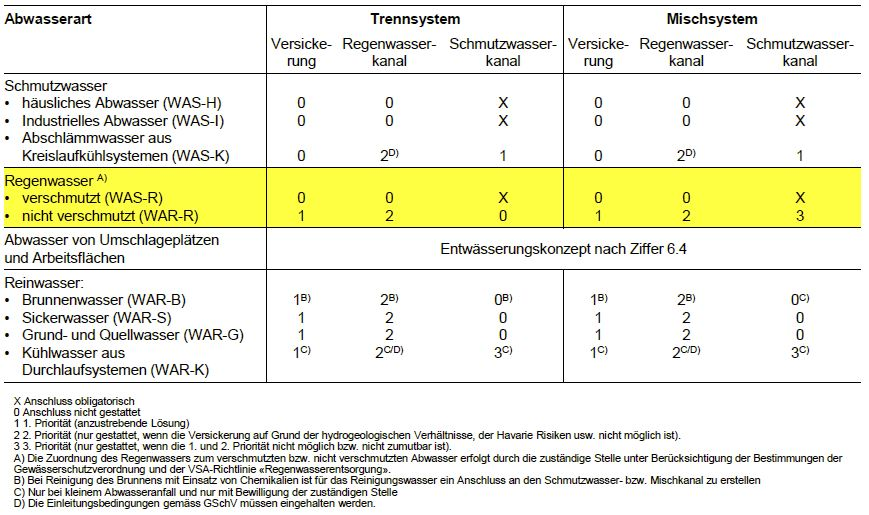
\includegraphics[width=\textwidth]{images/EntscheidEntwaesserung}
\label{Entwaesserungssystem}
\end{center}
\subsection{Aufgaben und Merkmale der Siedlungswasserwirtschaft}
\paragraph{Aufgabe} Die Aufgabe\index{Aufgaben} der Siedlungswasserwirtschaft\index{Siedlungswasserwirtschaft} ist das Bereitstellen von Trinkwasser und die langfristige Sicherung dieser Ressource. Eine weitere Aufgabe ist die Entsorgung von Schmutzwasser, Regenwasser sowie der anfallenden Schlämme und Fäkalien. Ziel ist es dabei die Gewässerbelastungen zu minimieren und den Lebensraum Gewässer zu erhalten.
\paragraph{Dienstleistungen} Die\index{Dienstleistungen} Dienstleistung der Siedlungswasserwirtschaft besteht darin, dass das Netz hygienisch, zuverlässig und wirtschaftlich ist. Weiter stellt sie Löschwasser für die Feuerwehr bereit.
\paragraph{Ressourcenverbrauch}\index{Ressourcenverbrauch} Für den Betrieb werden Baumaterialien, Betriebsmittel, Chemikalien, Energie, Kapital und Personal benötigt.
\paragraph{Wirtschaftszweig}\index{Wirtschaftszweig} Der Wirtschaftszweig der Siedlungswasserwirtschaft befasst sich mit der Produktion und dem Transport von Wasser sowie dem Bau, Betrieb und Erneuern der benötigten Infrastrukturen.\clearpage
\section{Wasserbilanz}
\index{Wasserbilanz}Die Schweiz wird häufig als Wasserschloss Europas bezeichnet. Der mittlere Niederschlag beträgt 1450 mm pro Jahr. Als\index{Abfluss!Definition} Abfluss wird der Niederschlag abzüglich der Verdunstung und den Veränderungen in den Speicher (Schnee, Gletscher, Seen, Grundwasser) verstanden.
\begin{center}
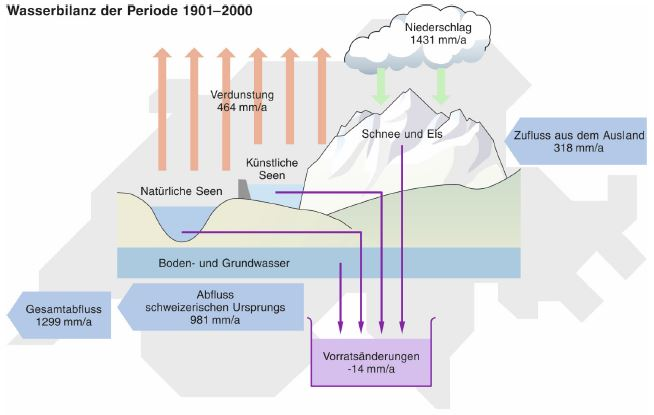
\includegraphics[width=.7\textwidth]{images/wasserbilanz}
\end{center}
Die Vorratsänderung von 14 mm/a in der obigen Abbildung ist auf den Gletscherschwund zurückzuführen. Neben diesem schweizweitem Wasserkreislauf können solche Bilanzen auch für Regionen erstellt werden. Im folgenden werden drei Bilanzen für verschiedene Bereiche gezeigt.
\paragraph{Landwirtschaft (Links)}\index{Wasserbilanz!Landwirtschaft} In der Landwirtschaft fliesst das Wasser natürlich ab. Ein Teil des Wassers fliesst oberflächlich ab und ein Teil versickert. Es ist damit ein direkter (diffuser) Abfluss von Niederschlagswasser in ein Gewässer.
\paragraph{Traditioneller Siedlungsraum (Mitte)}\index{Wasserbilanz!Traditioneller Siedlungsraum} Im traditionellen Siedlungsraum mit rund 50 Einwohner pro Hektare und einer Trennkanalisation fällt mehr als die Hälfte (60\%) des Wassers als Abwasser an. Zusätzlich wird Wasser (Trinkwasser) importiert.
\paragraph{Neuer Siedlungsraum (Rechts)}\index{Wasserbilanz!Neuer Siedlungsraum}
In Verdichteten Siedlungen mit mehr als 70 Einwohnern pro Hektare und Trennkanalisation wird der Wasserverbrauch reduziert. Der Import entfällt, da gleichviel Wasser an das Grundwasser zurückgegeben wird. Der Abwasseranteil liegt bei rund 50\%.
\begin{center}
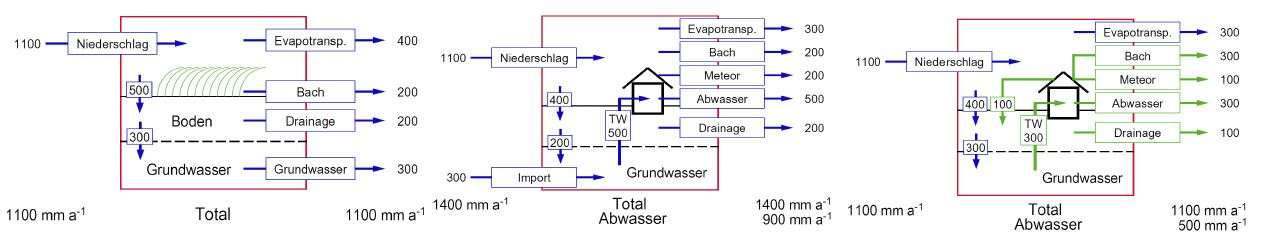
\includegraphics[width=\textwidth]{images/detailbillanzen}
\end{center}
Pro\index{Abwasseranfall} Einwohner fallen 850 Liter Abwasser pro Tag an. Das entspricht 140 mm pro Jahr oder 140 Liter pro Quadratmeter unter der Annahme einer mittleren Bevölkerungsdichte von 450 Einwohner pro Quadratkilometer des Schweizer Mittellands.  Davon sind mehr als 50\% Fremdwasser und Regenwasser. Die Bilanz wird jedoch stark durch die Gemeindegrösse und Siedlungsform beeinflusst. Pro Einwohner und Tag wird im mittel 2 Liter Wasser für das Trinken, 162 Liter für den Häuslichen Gebrauch und 400 Liter für Gewerbe und Industrie benötigt. Zusammen ergibt das 564 Liter, welches als Abwasser anfällt. Der Rest der 850 Liter sind Fremd- und Regenwasser! Im Schnitt rechnet man mit 200-300 Liter pro Tag und EW für den Abwasseranfall. Der Einwohnerwert EW dient zur Umrechnung der industriellen und gewerblichen Abwässer in den Abwasseranfall von Einwohnern.\\ \\
Aus dem\index{natürlicher Wasserhaushalt} natürlichen Wasserhaushalt: Niederschlag: 1100 mm/a (z.B. ZH), Evapotranspiration: -400 mm/a daraus folgt ein Abfluss von 700 mm/a und der urbanen Wassernutzung: 140 mm/a folgt die Wasserbilanz: Abfluss + Abwasser = 840 mm/a. Der \index{Abwasseranteil Gewässer}Abwasseranteil beträgt damit $140/ 840 = 17\%$. Dieser Abwasseranteil ist typisch in kleinen Gewässern. Bei Trockenwetter kann in einigen Gewässern der Schweiz der Abwasseranteil auf über 50\% ansteigen.
\section{Abflussbilanz}
Für die Erstellung einer \index{Abfluss!Abflussbilanz} Abflussbilanz muss zwischen Regen- und Trockenwetter unterschieden werden. Weiter muss zwischen dem effektiven Momentanwert und der Dimensionierungsgrösse differenziert werden. Bei Trockenwetter gilt:\[Q_t = Q_s + Q_f \textrm{    mit   } Q_s = Q_h + Q_g\]
Dabei ist $Q_t$ der Trockenwetterabfluss, $Q_s$ der Schmutzwasserabfluss, $Q_f$ der Fremdwasserabfluss, $Q_h$ häusliches Abwasser und $Q_g$ Abwasser aus Gewerbe und Industrie. Bei Regenwetter gilt:\[\textrm{Mischsystem: }Q_{ges} = Q_m = Q_t + Q_r\] Für das Trennsystem wird unterschieden zwischen Schmutzwasserkanal und Regenwasserkanal:\[\textrm{Schmutzwasserkanal: } Q_{ges} = Q_m = Q_t + Q_r \textrm{, Regenwasserkanal: } Q_{r,t} = Q_r\]
Dabei ist $Q_r$ der Regenwetterabfluss. Da die Abwassermenge $Q_h$ grossen Schwankungen unterliegt, wird zur Dimensionierung mit Faustzahlen gearbeitet (Linke Tabelle. Auch die Zuflüsse aus der Industrie und Gewerbe $Q_g$ gibt es Tabellenwerte für die Dimensionierung (Rechte Tabelle) 
\begin{center}
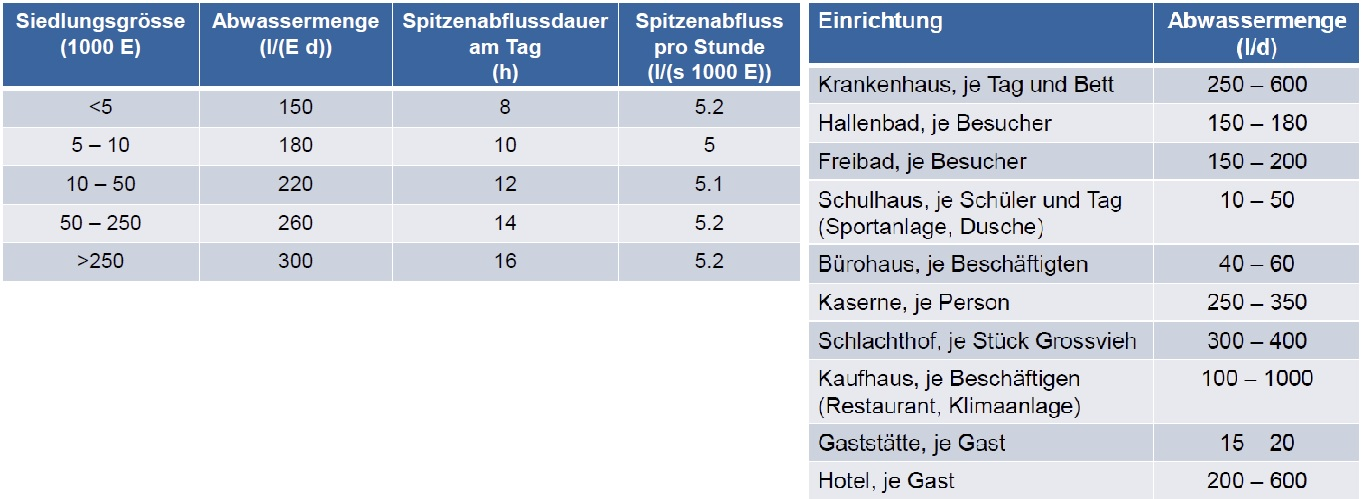
\includegraphics[width=\textwidth]{images/faustzahlenqh}
\end{center}\index{Abwassermengen}
Zwischen 50 und 70\% der privaten Abwasserleitungen sind sanierungsbedürftig. Unter anderem kommt es deshalb zu Fremdwasserzuflüssen $Q_f$. Diese bestehen aus Grundwasserinfiltration, Drainage- und Sickerwasser, Quell- und Bachwasser, Brunnenwasser, Kühlwasser und Wasser aus Wärmepumpen sowie Überlaufwasser aus Reservoirs. In der Schweiz haben die Gemeinden die Aufsichtspflicht über die privaten Abwasserleitungen. \\ \\
Der Regenwasserabfluss $Q_r$ ist massgebend für den Kanaldurchmesser. Das Regenabwasser kann nach dem Oberflächenabfluss kontaminiert sein. Bei zu viel Regenwasser kann es bei der Entlastung zu Schmutzwassereinträgen in die Oberflächengewässer kommen. Weiter wird der Kläranlagenbetrieb über das Regenereignis hinaus gestört und Kanalsedimente werden erodiert. Für die Bemessung muss der Regen beschrieben werden. In der Regel geschieht das als Blockregen (Bemessungsniederschlag). Dazu wird der Regen als gleichmässige Intensität über eine gewisse Zeit, als Block, modelliert. Die Regenintensität $r$ berechnet sich wie folgt: \[r = \dfrac{h_N}{t_N}\] mit der Regenhöhe $h_N$ in Millimeter und der Regendauer $t_N$ in Minuten (idR 5 bis 15 min).  Typische Einheiten für die Regenintensität sind mm/min oder l/(s mal ha).
\begin{center}
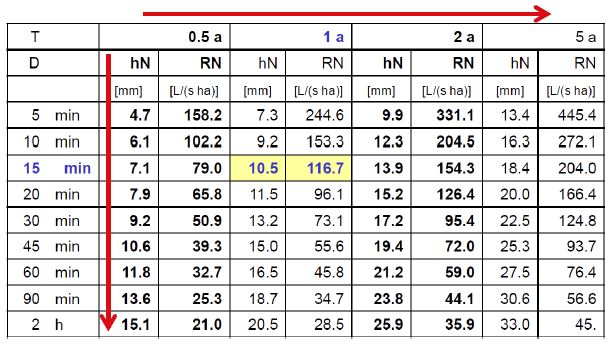
\includegraphics[width=0.5\textwidth]{images/RegendauervsIntensitaet}
\end{center}
Der Regen wird über die Dauer und die Wiederkehrperiode klassiert. Grundsätzlich gilt jedoch, dass bei gleicher Regendauer Schwachregen häufiger sind als Starkregen. Weiter sind bei gleicher Regenintensität kurze Regen häufiger als lang dauernde Regenereignisse. Häufig wird für die \index{Wiederkehrperiode Versickerung}Dimensionierung von Versickerungen eine Wiederkehrperiode z = 10 Jahre angesetzt. Weitere Beispiele bietet die untere Tabelle. Es ist anzumerken, dass die effektive Dimensionierung sowohl von der Risikoakzeptanz, als auch von den Kosten abhängt. Weiter gelten die Beispiele für vollgefüllte Systeme, welche nicht überlastet sind.\\ \par
\begin{table}[h]
\small
\begin{tabularx}{1\textwidth}{X C{0.2\textwidth} C{0.2\textwidth}}
\toprule
Gebiet & \multicolumn{2}{c}{Bemessungsregenhäufigkeiten} \\ 
 & Jährlichkeit z (a) & Überschreitungs-wahrscheinlichkeit je Jahr \\ 
\midrule 
Ländliche Gebiete, Strassen ausserhalb bebauter Gebiete & 1 & 100\% \\ 
Wohngebiete (allgemeine Bebauungsgebiete) & 2 & 50\% \\ 
Stadtzentren, Gewerbe- und Industriegebiete & 5 & 20\% \\ 
Unterirdische Verkehrsanlagen (Strassen/Autobahn, U-Bahn), Unterführungen & 10 & 10\% \\ 
\end{tabularx} 
\end{table}\par
Qualitativ verläuft die \index{Abfluss!Abflussbildung}Abflussbildung wie folgt: In einem ersten Schritt wird der Boden benetzt. Gleichzeitig verdunstet ein Teil des Niederschlags oder wird verweht. Nach der Benetzung setzt die Versickerung ein und die Mulden im Gelände werden bei grösserer Intensität gefüllt. In den übrigen Bereichen fliesst das Wasser oberflächlich ab.
\paragraph{Modellvorstellung zur Abflussbildung} Für die Dimensionierung von Entwässerungsanlagen, unter anderem Versickerungsanlagen, werden Modelle angewandt. Dabei ist der Abfluss eine Funktion von Niederschlag, Flächengrösse und Flächenmerkmalen. Die Flächenmerkmale sind in diesem Fall Abflussbeiwerte, welche in Abhängigkeit vom Niederschlag bestimmt werden. \[Q_R = r \cdot F \cdot \psi = r(t_{an} + t_{Fk,z}) \cdot \sum \gamma_i \cdot \alpha_i \cdot F_i \textrm{ mit } \psi = \sum \gamma_i \cdot \alpha_i \textrm{ und }\gamma_i = \dfrac{F}{F_{tot}}\] In dieser Formel ist $Q_R$ der \index{Abfluss!Regenwasserabfluss}Regenwasserabfluss, $r$ ist die Regenintensität und $\psi$ ist der Abflussbeiwert. Wie bereits erwähnt wird der spezifische mittlere \index{Abfluss!Mittlerer Abflussbeiwert}Abflussbeiwert $\psi_m$ (Abflusskoeffizient)\index{Abfluss!Abflusskoeffizient} abhängig vom Niederschlag berechnet. Dazu wird das Abflussvolumen durch das Niederschlagsvolumen geteilt:
\[\psi_m = \dfrac{V_{Abfluss}}{V_{Niederschlag}} = \dfrac{\int Q_R \cdot dt}{\int r \cdot F \cdot dt}\]
Der \index{Abfluss!Spitzenabflussbeiwert}Spitzenabflussbeiwert $\psi_S$ ist ein Transferkoeffizient. Er wird mit einem Blockregen mit einer konstanten Regenintensität $r_{max}$, mit einer definierten Wiederkehrperiode und dem Spitzenabfluss $Q_{r,max}$ berechnet. Dieser Koeffizient gibt an, wie viel Prozent vom Regenanfall beim Spitzenabfluss in die Kanalisation gelangt. Er wird daher für die Dimensionierung der Kanäle benötigt. \[\psi_S = \dfrac{Q_{R,max}}{r_{max} \cdot F} \textrm{  oder  } Q_{R,max} = r_{max} \cdot F \cdot \psi_S\]\index{Abfluss!Abfluss als Funktion von}
Typische Werte für $\psi_S$ sind: Einfamilienhäuser mit Versickerung 0.15, mit Flachdächern 0.20, mit Steildächern 0.25; Wohn- und Gewerbezonen 0.70, City / Altstadt 0.75\\ \\
Das Ziel ist es den Spitzenabfluss $Q_{r,max}$ zu minimieren. Folgende Möglichkeiten sind denkbar:
\begin{itemize}
\item Längere Anlaufzeiten durch begrünte Dächer, Retention
\item Häufigere gezielte Überschwemmungen zulassen, einzelne Felder, Parkplätze
\item Teilflächen zur Förderung der Versickerung von Dachwasser
\item Kleine Abflussbeiwerte, z.B. durchlässige Beläge, Rasengittersteine
\item Verdichtetes Bauen
\end{itemize}
Der maximale\index{Abfluss!Abflusskoeffizient} Abflusskoeffizient ist im GEP festgehalten. Ist der Abflusskoeffizient der Parzelle zu gross, muss versickert werden oder eine Retentionsanlage gebaut werden.\\ \\
Der \index{Abfluss!Dauerabflussbeiwert}Dauerabflussbeiwert ist nicht gleich dem Spitzenabflussbeiwert. Er stellt einen Mittelwert über zwei Jahre dar. Beide Beiwerte sind massgeblich vom Dachtyp und Dachaufbau abhängig. Beide weisen Schwankungen auf durch Witterungseinfluss und Niederschlagsverteilung. Deshalb muss häufig noch ein Sicherheitsfaktor berücksichtigt werden.\index{Abfluss!Tabelle Abflussbeiwerte}
\begin{center}
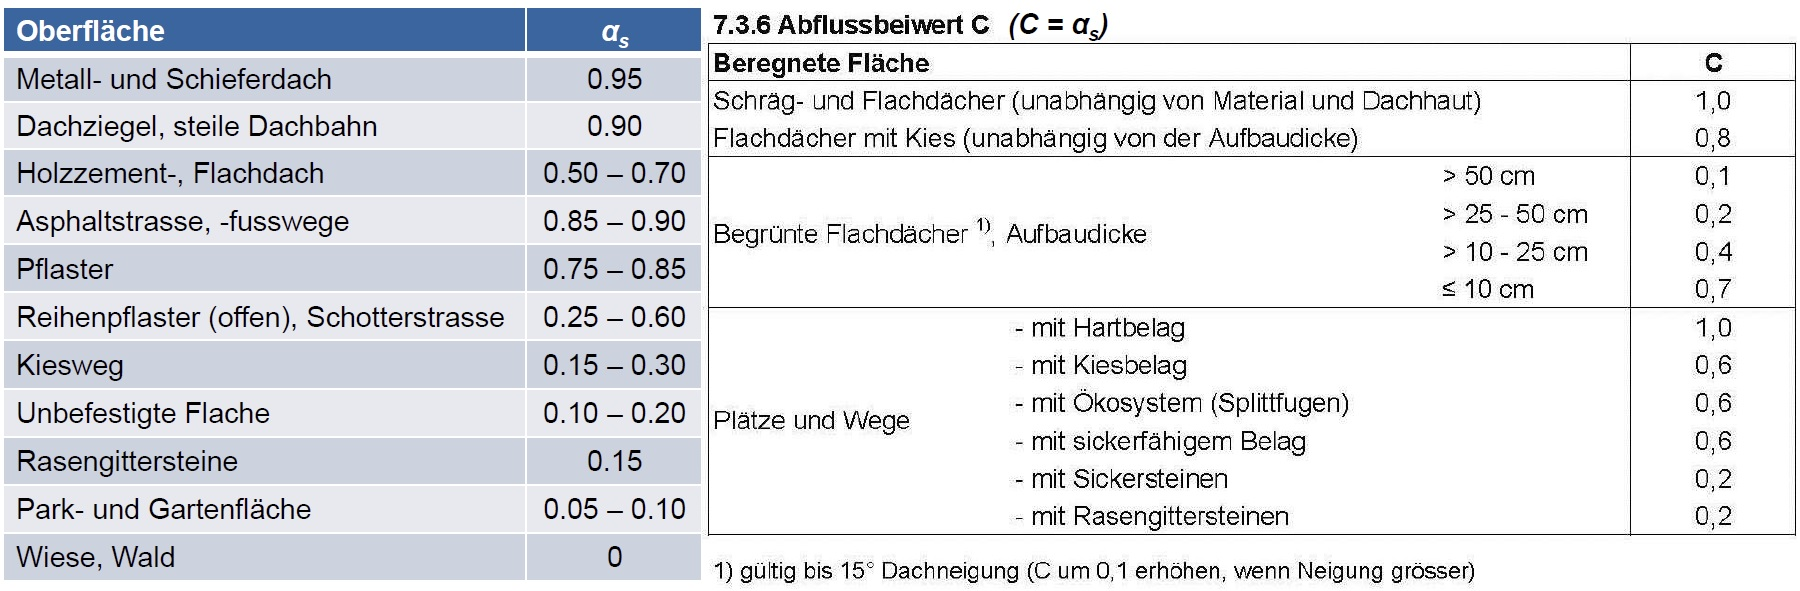
\includegraphics[width=\textwidth]{images/beiwerte}
\end{center}\par 
Beispiel Trockenwetter- und Regenwetterabfluss:
\begin{center}
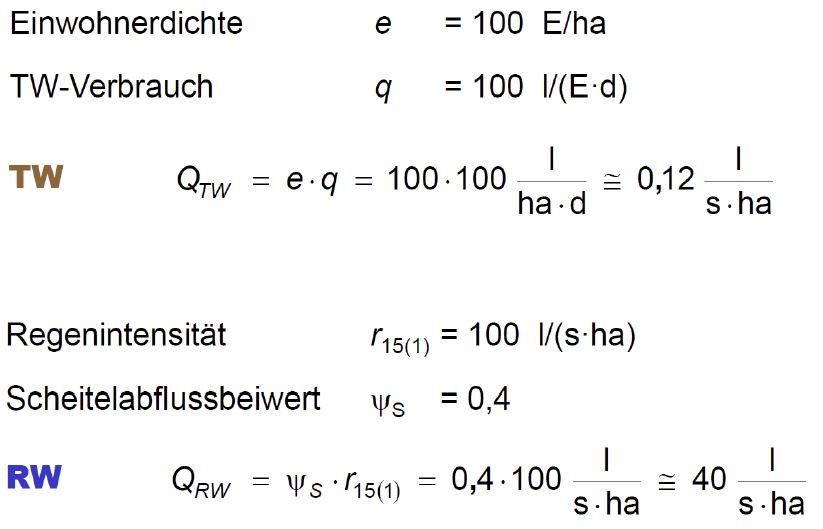
\includegraphics[width=0.5\textwidth]{images/BeispielBilanz}
\end{center}\index{Abfluss!Beispielrechnung}
Um die Fliesszeiten zu berücksichtigen werden meist Listenrechnungen gemacht (z.B. nach Imhof). Typische Werte für die Anlaufzeit sind zwei bis zehn Minuten. In der Schweiz meist fünf Minuten.
\section{Schadstoffe und Quellen}
\subsection{Ausgangslage - Abwasser}
Häufig gelangen\index{Schadstoffe} Schadstoffe aus Industrie und Gewerbe in die Kanalisation. Verschiedene Branchen\index{Schadstoffe!Quellen} erzeugen Abwässer: Pigmentherstellung, Metallverarbeitung (z.B. Galvanik), Wäschereien, Nahrungsmittel-, Textil-, Glasindustrie etc. Dabei sind die Branchenspezifischen Grenzwerte gemäss Gewässerschutzverordnung zu beachten. Diese Abwässer werden in die Kläranlage geleitet. Meist ist jedoch eine Vorreinigung erforderlich.\index{Schadstoffe!Typische Schadstoffe} Typische Schadstoffe aus Gewerbe und Industrie sind:
\begin{itemize}
\item Gelöste Metalle, kationisch: Cu, Ni, Pb, Zn, Cd, Hg; anionisch: Chromat, Arsenat
\item Salze, anionisch: Sulfat, Chlorid, Phosphat, Nitrit etc.
\item Komplexbildner; EDTA, Cyanide, Aminoverbindungen, Carboxylate etc.
\item Kohlenwasserstoff: CKW, MKW etc.
\item Tenside / Emulgatoren, Netzmittel, Flammschutzmittel, Weichmacher etc.
\end{itemize}
\subsection{Rechtliche Rahmenbedingungen in der Schweiz}
Die\index{Schadstoffe!Rechtliche Aspekte} Rechtlichen Rahmenbedingungen liefern das Gewässerschutzgesetz (GSchG) und die Gewässerschutzverordnung (GSchV). Im folgenden einige Definitionen gemäss Artikel 4, GSchG. Oberirdisches Gewässer: Wasserbett mit Sohle und Böschung sowie die tierische und pflanzliche Besiedlung; Unterirdisches Gewässer: Grundwasser (einschl. Quellwasser), Grundwasserleiter, Grundwasserstauer und Deckschicht; Nachteilige Einwirkung: Verunreinigung und andere Eingriffe, welche die Gestalt oder die Funktion eines Gewässers beeinträchtigen; Verunreinigung: Nachteilige physikalische, chemische oder biologische Veränderung des Wassers; Abwasser: Das durch häuslichen, industriellen, gewerblichen,
landwirtschaftlichen oder sonstigen Gebrauch veränderte Wasser, ferner das in der Kanalisation stetig damit abfliessende Wasser sowie das von bebauten oder befestigten Flächen abfliessende Niederschlagswasser; Verschmutztes Abwasser: Abwasser, das ein Gewässer, in das es gelangt, verunreinigen kann.\paragraph{Artikel 70, GSchG} Mit Freiheitsstrafe bis zu drei Jahren oder Geldstrafe wird bestraft, wer vorsätzlich Stoffe, die das Wasser verunreinigen können, wiederrechtlich mittelbar oder unmittelbar in ein Gewässer einbringt, versickern lässt oder ausserhalb eines Gewässers ablagert oder ausbringt und dadurch die Gefahr einer Verunreinigung des Wassers schafft.\paragraph{Artikel 3, GSchV} Die Behörde beurteilt, ob Abwasser bei der Einleitung in ein Gewässer oder bei der Versickerung als verschmutzt oder nicht \index{Schadstoffe!Beurteilung}verschmutzt gilt, auf Grund:a.) der Art, der Menge, der Eigenschaften und des zeitlichen Anfalls der Stoffe, die im Abwasser enthalten sind und Gewässer verunreinigen können; b.) des Zustandes des Gewässers, in welches das Abwasser gelangt.\\ Bei der Versickerung von Abwasser berücksichtigt sie ausserdem, ob: a.) das Abwasser wegen der bestehenden Belastung des Bodens oder des nicht wassergesättigten Untergrundes verunreinigt werden kann; b.) das Abwasser im Boden ausreichend gereinigt wird; c.) die Richtwerte der Verordnung vom 1. Juli 1998 über Belastungen des Bodens (VBBo) langfristig eingehalten werden können, ausgenommen bei der Versickerung in einer dafür bestimmten Anlage oder an Verkehrswegen im Bereich der Böschungen und der Grünstreifen.\\ Von bebauten oder befestigten Flächen abfliessendes Niederschlagswasser gilt in der Regel als nicht verschmutztes Abwasser, wenn es: a.) von Dachflächen stammt; b.) von Strassen, Wegen und Plätzen stammt, auf denen keine erheblichen Mengen von Stoffen, die Gewässer verunreinigen können, umgeschlagen, verarbeitet und gelagert werden, und wenn es bei der Versickerung im Boden ausreichend gereinigt wird; bei der Beurteilung, ob Stoffmengen erheblich sind, muss das Risiko von Unfällen berücksichtigt werden; c.) von Gleisanlagen stammt, bei denen langfristig sichergestellt ist, dass auf den Einsatz von Pflanzenschutzmitteln verzichtet wird, oder wenn Pflanzenschutzmittel bei der Versickerung durch eine biologisch aktive Bodenschicht ausreichend zurückgehalten und abgebaut werden.\\ \\
Die Anforderungen an die Wasserqualität sind in Anhang 2 der Gewässerschutzverordnung festgehalten. Dabei gelten die folgenden Allgemeinen Anforderungen: Durch Abwassereinleitungen darf sich im Gewässer nach weitgehender Durchmischung:a.) kein Schlamm bilden; b.) keine Trübung, keine Verfärbung und kein Schaum bilden, ausgenommen bei starken Regenfällen; c.) der Geruch des Wassers gegenüber dem natürlichen Zustand nicht störend verändern; d.) kein sauerstoffarmer Zustand und kein nachteiliger pH-Wert ergeben.
\subsection{Parameter zur Charakterisierung und Einstufung}
Folgende Grafik zeigt eine Übersicht über die Wasserinhaltsstoffe und mögliche Behandlungsverfahren.\\
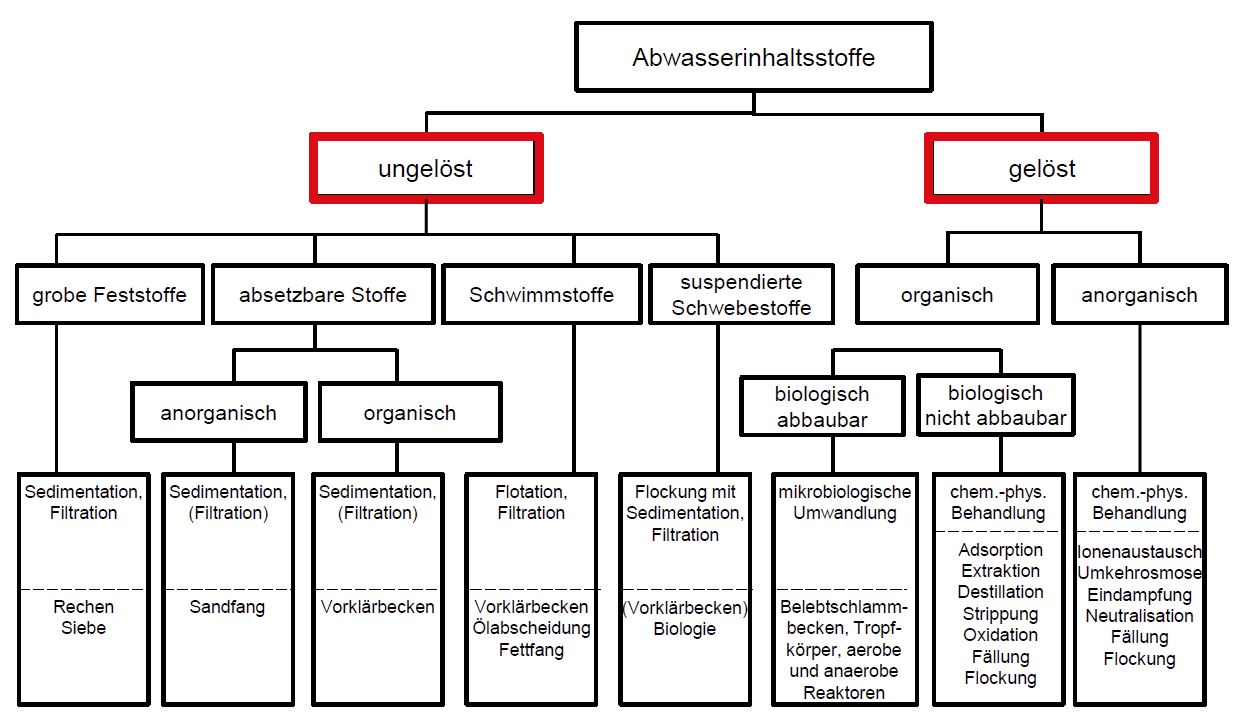
\includegraphics[width=\textwidth]{images/inhaltbehandlung}\index{Wasserinhaltsstoffe}\index{Behandlungsverfahren}
Das Abwasser liefert Energie für die Mikroorganismen, welche wachsen und sich vermehren. Der Abbau bedeutet gleichzeitig eine Sauerstoffzehrung womit sauerstofflose, anaerobe Zustände entstehen. Partikuläre organische Stoffe können aussedimentieren und es kommt zu einer Verschlammung. Ebenfalls kann das Abwasser toxische Stoffe enthalten. \paragraph{Physikochemische Parameter} Dazu gehören viele Parameter wie zum Beispiel der\index{pH-Wert} pH-Wert, welcher unter anderem die Löslichkeit von Salzen und Metallen aber auch die Aktivität von Mikroorganismen stark beeinflusst. Das Abwasser hat meist einen pH-Wert zwischen 7.2 und 8.3. Damit es in ein Gewässer eingeleitet werden kann, muss der pH-Wert zwischen 6 und 9 liegen. Weitere Parameter sind: \index{Elektrische Leitfähigkeit}Elektrische Leitfähigkeit, \index{Trübung}Trübung / Durchsichtigkeit, Temperatur, Dichte, Viskosität, Oberflächenspannung, Geruch, Geschmack. Zusammen mit der Lufttemperatur nimmt auch die Wassertemperatur stetig zu. \paragraph{Partikuläre Stoffe im Wasser} Häufig trifft man auf den Parameter der\index{gesamte ungelöste Stoffe (GUS/TSS)} gesamten ungelösten Stoffe (GUS) oder \index{abfiltrierbare Stoffe (AFS)}abfiltrierbare Stoffe (AFS). Wobei gelösten Stoffe auch bei uns meist als\index{Total Suspended Solids (TSS/GUS)} Total Suspended Solids (TSS) bezeichnet werden. Es handelt sich dabei nicht um einen chemisch eindeutig definierten Parameter sondern um einen \index{Summenparameter}Summenprameter zum Vorkommen von Partikeln. Er wird gravimetrisch bestimmt, nachdem das Wasser mit einem Membranfilter (Porengrösse 0.45 $\mu$m) gefiltert wurde und die Probe bei 105 Grad getrocknet wurde. Im Moment fehlen Analytische Routinemethoden zur Erfassung von Einzelpartikeln. Die \index{GUS!Anforderungen}Anforderung gemäss GSchV sind für kommunales Abwasser aus einer ARA $<$ 10'000 EW 20mg/l und aus einer ARA $>$ 10'000 EW 15 mg/l. Die GUS \index{GUS!Zusammensetzung}setzen sich zusammen aus natürlichen mineralischen Primärpartikeln und Fällungsprodukten (Tonminerale, Eisenhydroxide, Karbonate etc.). Weiter \index{GUS!Ursprung}sind natürliche biologische Partikel und Abbauprodukte enthalten wie Algen, Pflanzenreste, Tierkot etc. Aber auch synthetische Partikel aus Anwendungen und Prozessen (Pneu- und Bremsabrieb, Russ, Farbpigmente etc.) können als GUS im Abwasser vorkommen. Vor allem der Pneuabrieb stellt ein grosses Problem dar. Er enthält über 200 verschiedene, meist Organische, Stoffe. Darunter Kautschuk, Zink-, Bleioxide, Öle, Schwefel und viele andere. Die GUS werden weiter unterteilt in\index{Glühverlust (GV/VSS)} Glühverlust (GV, engl. VSS), \index{Glührückstand (TR)}Glührückstand (TR) und \index{Trockensubstanz (TS)}Trockensubstanz (TS). Der Glühverlust wird bestimmt, indem die GUS nach der Filtration bei 650 Grad geglüht und der Gewichtsverlust bestimmt wird. Es ist ein Mass für die Biomasse, da der verglühte Anteil etwa der organischen Substanz entspricht. Er hat damit eine zentrale Bedeutung für die Sauerstoffzehrung. Der Glührückstand ist das, was beim Glühen zurückbleibt. Es ist somit der mineralische Rest. Bei der Bestimmung der Trockensubstanz findet keine Filtration statt. Damit sind auch die gelösten Salze eingeschlossen. Da im Abwasser der unterschied zwischen TS und GV sehr gross ist (Faktor 2) werden die Glühverluste bestimmt. Im Klärschlamm hingegen ist die Differenz sehr gering (häufig kleiner 10\%). Auch kann der Klärschlamm nur schlecht filtriert werden, weswegen hier in der Regel die Trockensubstanz bestimmt wird.
\paragraph{Gase im Wasser} \index{Gase im Wasser}Im Wasser sind viele Gase gelöst. Im folgenden werden drei vorgestellt. Sauerstoff ($O_2$) wird beim Abbau von organischer Substanz und bei oxidativen Prozessen verbraucht. \index{Sauerstoff}Sauerstoff beeinflusst damit die biologische Aktivität und die Umwandlung von Stoffen (gelöst zu ungelöst). Der Sauerstoffgehalt ist in einem mit Wasserpflanzen bewachsenen Gewässer am Tag am höchsten (Photosynthese). Bei 20 Grad im gesättigten Wasser ist so 8-9 mg/l Sauerstoff enthalten. In technischen Prozessen wird das Wasser belüftet für den aeroben Abbau von Stoffen (zum Teil auch in Seen). \index{Kohlendioxid}Kohlendioxid ($CO_2$) ist ein Stoffwechselprodukt der Atmung. Das Gas hat einen starken Einfluss auf das \index{Kalk-Kohlensäure-Gleichgewicht}Kalk-Kohlensäure-Gleichgewicht und den \index{pH-Wert}pH-Wert (z.B. Baustellenabwasser).\[2 NaOH + CO_2 \Leftrightarrow Na_2CO_3 + H_2O \rightarrow Na_2CO_3 + H_2O + CO_2 \Leftrightarrow 2 NaHCO_3 \] Es kommt zu sichtbaren Ausfällungen (Tropfsteine etc.) und zur Lösung von Kalk. Das dritte Gas ist \index{Schwefelwasserstoff}Schwefelwasserstoff ($H_2S$). Es ist geruchsintensiv und giftig. Es kommt auch in anaeroben Bedingungen vor und ist eine schwache Säure (pKs 6.9). Da es Betonkorrosion verursacht, kann es ganze Kanalisationsteile schädigen oder zerstören.
\paragraph{Biochemischer Sauerstoffbedarf $BSB_5$}\index{Biochemischer Sauerstoffbedarf BSB\textsubscript{5}} Gibt die Menge Sauerstoff ($O_2$) an, welche Mikroorganismen bei 20 Grad unter Lichtausschluss innerhalb von 5 Tagen verbrauchen um organische Stoffe abzubauen. Es ist daher ein\begin{wrapfigure}{r}{8cm} 
  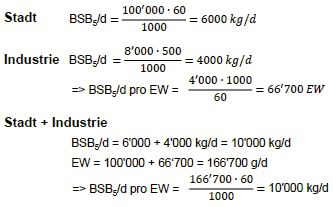
\includegraphics[width=.5\textwidth]{images/AufgabeBSB}
\end{wrapfigure} \index{BSB\textsubscript{5} Beispiel}Summenparameter für biologisch abbaubare organische Stoffe, insbesondere für Kohlenstoff-Verbindungen. Eine grosse Belastung solcher Stoffe führt zu einer starken Sauerstoffzehrung im Gewässer. Im Fliessgewässer beträgt der BSB\textsubscript{5}-Sauerstoffbedarf etwa 2 bis 4 mg/l. Der Schweizer Richtwert\index{BSB\textsubscript{5} Richtwerte} für Abwasser liegt bei 60 g BSB\textsubscript{5}/Tag bei 170 Liter pro Einwohner. Im Zulauf der ARA ist der Wert mit 200 - 400 mg/l deutlich höher. Im Ablauf fordert die GSchV für ARAs $<$ 10'000 EW einen Wert von 20 mg/l und für ARAs $>$ 10'000 EW einen Wert von 15 mg/l. Die Messung dauert fünf Tage bei 20 Grad. Zusätzlich muss die Probe dunkel gelagert und mit Sauerstoffreichem Wasser verdünnt werden. Zusätzlich wird eine Biomasse angeimpft wodurch der Sauerstoffhalt durch die Bakterien sinkt und CO\textsubscript{2} gebildet wird. Da nicht alle organischen Stoffe biologisch abbaubar sind und ein Teil der organischen Stoffe in die Mikroorganismen eingebaut werden, gilt: $BSB_5 < CSB$. \\ Beispiel Rechts: Stadt 100'000 EW, 60 g BSB\textsubscript{5}/(E und Tag) und Industrie mit vergleichbarer Abwasserqualität: 8000 m\textsuperscript{3}, 500 g BSB\textsubscript{5}/(E und Tag). Gesucht wird kg-Bedarf an BSB\textsubscript{5}/Tag. Beispiel 2: Gesucht Einwohnerwert EW. Gegeben: BSB\textsubscript{5}-Bedarf pro Tag in kg. Lösung: EW = BSB\textsubscript{5}-Bedarf pro Tag in kg mal 1000 geteilt durch 60 g BSB\textsubscript{5}/(E und Tag).\\
\paragraph{Chemischer Sauerstoffbedarf $CSB$}\index{Chemischer Sauerstoffbedarf CSB} Beschreibt die vollständige Oxidation fast aller organischer Stoffe zu CO\textsubscript{2} und H\textsubscript{2}O und damit nicht nur die biologisch abbaubaren Stoffe. In der Umwelt ist eine starke Sauerstoffzehrung\begin{wrapfigure}{r}{8cm} 
  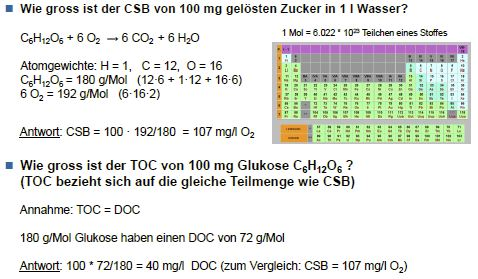
\includegraphics[width=.5\textwidth]{images/AufgabeCSBTOC}
\end{wrapfigure}\index{CSB Beispiel} ein Hinweis für Schadstoffe im Abwasser und Sauerstoffmangel. Der Schweizer Richtwert für Abwasser liegt bei 120 g CSB/Tag bei 170 Liter pro Einwohner. Gemäss GSchV gilt für ARAs $<$ 10'000 EW ein Wert von 60 mg/l O\textsubscript{2} und für ARAs $>$ 10'000 EW ein Wert von 45 mg/l O\textsubscript{2}, was einer Elimination von 85\% entspricht. Das Verhältnis BSB\textsubscript{5}/CSB \index{CSB Richtwerte}liegt im Zulauf einer ARA bei etwa 0.6 und im Ablauf bei 0.2. Der relative Anteil an nicht-abbaubaren organischen Inhaltsstoffen nimmt also zu. Gemessen wird der CSB mittels Titration des Oxidationsmittels Kaliumdichromat ($K_2Cr_2O_7$) in Schwefelsäure. Weiter gibt es sogenannte Küvetten-Schnelltests.
\paragraph{Nährstoffe - Kohlenstoff} Hier wird zwischen dem\index{Totaler organischer Kohlenstoff TOC} Totalen organischen Kohlenstoff (TOC) und dem\index{Gelöster organischer Kohlenstoff DOC} gelösten organischen Kohlenstoff (DOC) unterschieden. Dieser hat natürliche und anthropogene Quellen. Der gelöste Kohlenstoff wird nach einer Filtration gemessen. Weiter hat er die Eigenschaft Metalle zu binden und damit zu verlagern. Ausserdem ist er Sauerstoffzehrend. Im Fliessgewässer liegt\index{DOC Richtwerte} DOC-Wert bei 1-4 mg/l C und im Ablauf der ARA 10 mg/l und 85\% Elimination.
\paragraph{Nährstoffe - Stickstoffverbindungen}\index{Biomasse} Biomasse enthält zirka 4 bis 7\% Stickstoff (vor allem in Proteinen und Eiweissen). Der Abbau organischer Stickstoffverbindungen setzt $NH_4^+$ (Ammonium) frei. Das Nitrat im Wasser\begin{wrapfigure}{l}{8cm} 
  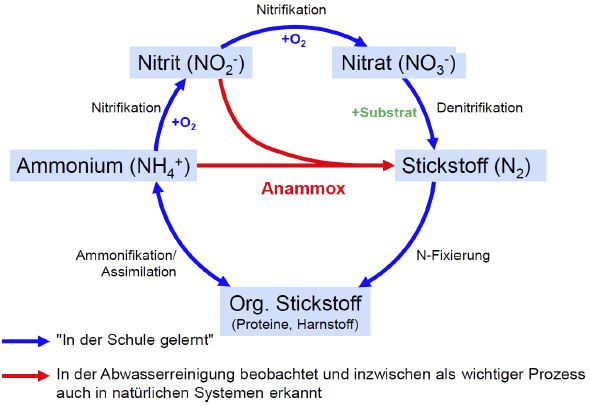
\includegraphics[width=.5\textwidth]{images/Nitrifikation}
\end{wrapfigure} stammt \index{Nitrifikation} \index{Denitrifikation}vorrangig aus der Landwirtschaft. Die Folgen für das Gewässer sind Überdüngung, Abbau von\index{Ammonium} Ammonium zu \index{Nitrit}Nitrit ($NO_2^-$) und\index{Nitrat} Nitrat ($NO_3^-$) zehrt Sauerstoff (Nitrifikation). Ammoniak und Nitrit gelten als Fischgift und schädigen so die Gewässer. Weiter gelangt Nitrat ins Trink- und Grundwasser. Ammonium ($NH_4^+$) und \index{Ammoniak}Ammoniak ($NH_3$): Das Verhältnis zwischen Ammonium und Ammoniak ist temperatur- und pH-abhängig. Höhere Temperaturen und pH-Werte führen zu höheren Anteilen von Ammoniak. In Fliessgewässern liegt der\index{Ammoniak Richtwerte} Wert bei 0.2 mg/l ($>$ 10 Grad, Summe $NH_4^+$-N und $NH_3$-N). Die Abflusskonzentration in der ARA liegt bei 2mg/l und einer Reinigungsleistung von 90\%. Nitrat ($NO_3^-$) und Nitrit ($NO_2^-$): Werden aus Ammonium und Ammoniak gebildet. $NH_4^+ + NH_3 \Rightarrow NO_2^- \Rightarrow  NO_3^-$. In Fliessgewässern beträgt die Konzentration 5.6 mg/l N oder gleich 25 mg/l $NO_3^-$. Das Endprodukt der Denitrifikation (Nitrat zu Stickstoff) bildet Elementarer Stickstoff $N_2$. Dieser ist gasförmig und bildet als $NO_2$ den Hauptanteil der Gase in der Atmosphäre. In der Biologischen Stufe der ARA tritt es als Gas aus, da es schlecht Wasserlöslich ist. Die Summe aller organischer Stickstoffverbindungen lässt sich mit dem Summenparamter\index{Totaler Kjeldhal Stickstoff (TKN)} Totaler Kjeldhal Stickstoff (TKN) beschreiben. Nach der chemischen Oxidation mit konzentrierter Schwefelsäure wird der Ammoniumgehalt bestimmt. Im Rohabwasser liegt fast der gesamte Stickstoff als TKN vor, im biologisch behandelten Abwasser vor allem als Nitrit oder Nitrat.
\paragraph{Nährstoffe - Phosphor}\index{Phosphor} Organischer Phosphor ist ein Bestandteil der DNA und der RNA. Er kommt aber auch in der Landwirtschaft (Dünger), in Haushaltsabwasser etc. vor. In der Umwelt führt der Phosphor zu einer eutrophierung der Gewässer, also einer Überdünung und damit zu Algenwachstum. Der Totale Phosphor (TP, $P_{tot}$) besteht aus gelösten und partikulären Anteilen. Gelöster Phosphor ist das Anion Orthophosphat ($PO_4$-P), welches in Salzen der Phosphorsäure vorkommt (z.B. $H_3PO_4$). Es wird durch Adsorption/Fällung, durch Filtration und durch den Einbau in die Biomasse zurückgehalten. Die Messung findet nach der Mineralisierung statt. Heute sind 97\% der kommunalen Abwässer mit P-Elimination gereinigt. 
\paragraph{Metalle - Kupfer, Nickel, Zink etc.}\index{Metalle} Die Metalle stammen sowohl aus geogenen Quellen als auch aus anthropogenen Quellen. In der Umwelt sind sie nicht abbaubar und die gelösten Anteile sind toxisch (z.B. $CU^{2+}$. Deshalb gibt es Anforderungen sowohl für den gelösten Anteil, als auch für den Gesamtanteil. Der Rückhalt erfolgt mittels Adsorption, Fällung und Filtration. Metalle können analytisch nachgewiesen werden mit folgenden Methoden: \index{AAS} AAS, \index{ICP-OES} ICP-OES,\index{ICP-MS} ICP-MS.
\paragraph{Mikroverunreinigungen} \index{Mikroverunreinigungen} In der Schweiz gibt es zirka 30'000 synthetische und organische Stoffe wie Pharmaka, Pflanzenschutzmittel, Biozidprodukte und Industriechemikalien sowie Schwermetalle. Dabei sind die Stoffe in vielerlei Hinsicht gefährlich. Einige sind\index{hormonaktiv} hormonaktiv,\index{preresistent} preresistent,\index{bioakkumulativ} bioakkumulativ oder mobil. Die Wirkung ist abhängig von der Substanz, der Konzentration und dem Organismus. Pflanzenschutzmittel müssen in der\index{Pflanzenschutzmittelverordnung (PSM-Verordnung)} PSM-Verordnung zugelassen sein. Es sind über 450 Wirkstoffe bekannt und der Verbrauch beträgt in der Schweiz zirka 2000 Tonnen\begin{wrapfigure}{r}{8.3cm} 
  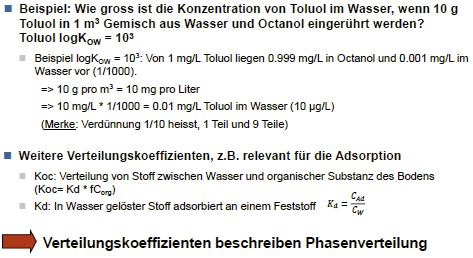
\includegraphics[width=.55\textwidth]{images/BeispielKOW}
\end{wrapfigure} pro Jahr. Eingesetzt\index{Verteilungskoeffizient (K\textsubscript{OW})!K\textsubscript{OW} Beispiel} werden sie vor allem in der Landwirtschaft und im Siedlungsbereich. Die Zulassung von \index{Biozidprodukte}Biozidprodukte ist in der VBP geregelt. Es sind rund 400 Wirkstoffe und 23 Produktarten (PA) bekannt. Der Verbrauch in der Schweiz liegt bei zirka 1000 Tonnen pro Jahr für Innen- und Aussenanwendungen. Es sind Wirkstoffe, die chemisch oder biologisch Schadorganismen kontrollieren oder zerstören. Die Anforderungen für Gewässer liegen bei 0.1 Mikrogramm pro Liter für Pestizide. In den Bauprodukten kommen immer mehr organische Stoffe zum Einsatz.
\paragraph{Verteilungskoeffizient $K_{OW}$}\index{Verteilungskoeffizient (K\textsubscript{OW})} Er beschreibt die Stoffverteilung zwischen n-Octanol und Wasser. n-Octanol ist sowohl hydrophob als auch lipophil.\index{hydrophob}\index{lipophil}\index{hydrophil}\index{lipophob} Wasser hingegen ist hydrophil und lipophob. Der Logarithmus von $K_{OW}$ ist für hydrophile / lipophobe negativ und für hydrophoben / lipophilen positiv. Er ist ein Indikator für die Anreicherung in Organismen und für den Rückhalt im Boden, Klärschlamm und Sediment. Tenside sind Lösungsvermittler für lipophile Stoffe, welche so bioverfügbar werden. 
\subsection{Anforderungen an die Ableitung von verschmutztem
Abwasser}
\begin{center}
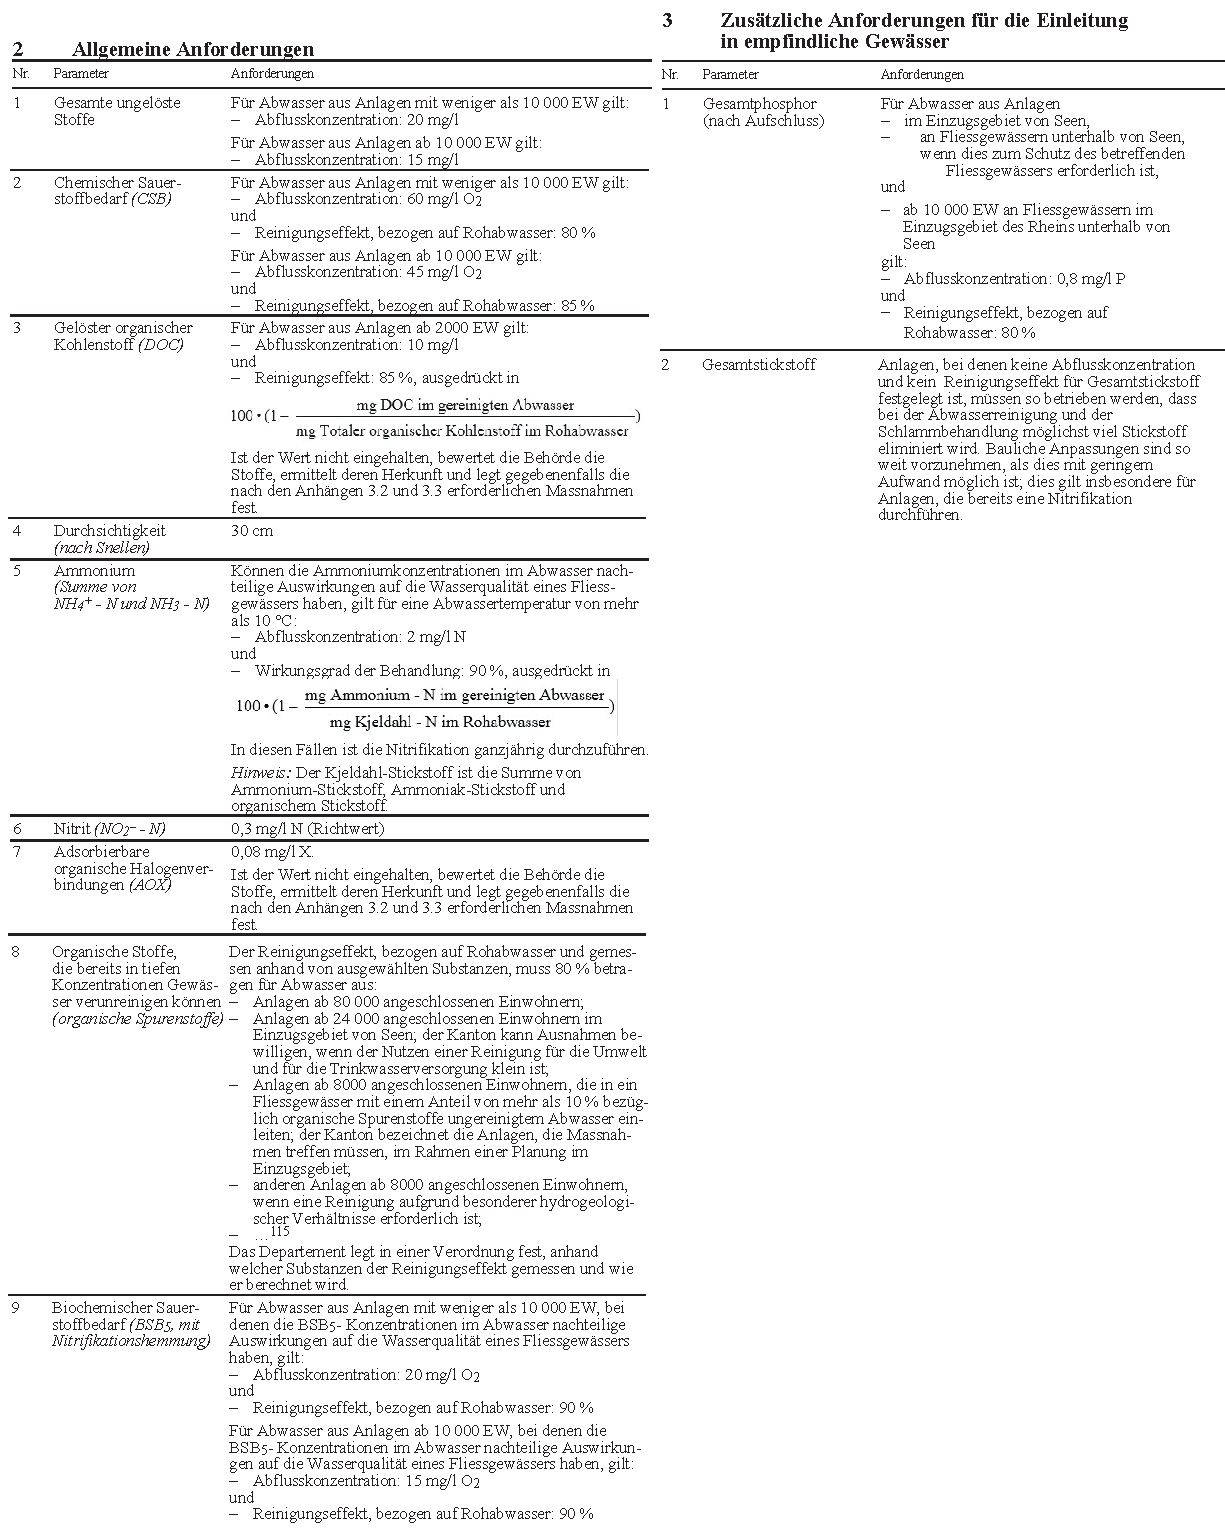
\includegraphics[width=1.00\textwidth]{images/anhgschv}
\end{center}
\begin{small}
Quelle: Gewässerschutzverordnung GSchV, Anhang 3
\end{small}
\section{Eintragswege und Fracht}
Unter\index{Emission Definition} Emission versteht man die Freisetzung ins Schmutz- und Niederschlagswasser. Unter \index{Immission Definition}Immission das\begin{wrapfigure}{r}{8cm} 
  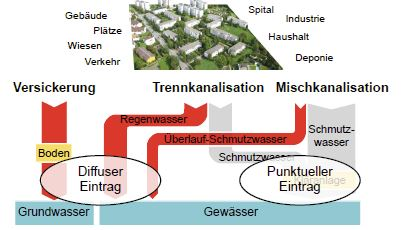
\includegraphics[width=.5\textwidth]{images/Eintrag}
\end{wrapfigure} Vorkommen von Stoffen in Umweltkompartimenten. Die\index{Fracht} Fracht oder\index{Stoffmenge} Stoffmenge ist gleich der Konzentration mal der Wassermenge. Der \index{Frachtverlauf}Frachtverlauf ist dabei von vielen Faktoren abhängig. Bei punktuellen Einträgen findet dieser kontinuierlich statt und bei Regenwetter wird der Stoff verdünnt. Bei diffusen Einträgen erfolgt der Eintrag erst bei Regenwetter. Die Probenahme solcher diffusen Einträge gestaltet sich sehr schwierig. Im Boden und in Sedimenten sammeln sich Stoffe an und die Konzentration nimmt über die Zeit ständig zu. Die dynamischen Einflüsse von Regenereignissen haben praktisch keinen Einfluss. In Gewässern wird eine grosse Konzentration schnell verdünnt. Auf dem Diagramm bildet sich damit erst eine Spitze, welche dann rasch abflacht. Bisher wurde für die Abwasserbeurteilung immer eine Emissions-Betrachtung gemacht, also wie viel darf in ein Gewässer eingeleitet werden. Neu strebt man eine Immissions-orientierte Betrachtung an. Dazu gibt es die\index{Richtlinie STORM} Richtlinie STORM des VSA. Dabei wird betrachtet, wie viel ein Gewässer verträgt. Die Einleitbedingungen berücksichtigen damit auch das Mischungsverhältnis im Vorfluter. Als Voraussetzungen für STORM braucht man Kenntnisse über stoffliche und hydraulische Belastungen im Gewässer. Dazu sind Langzeitsimulationen notwendig. Nicht immer ist der Bau eines Regenüberlaufbeckens die beste Lösung!
\subsection{Schmutzabwasser}
In der folgenden Abbildung sind die Emissionen verschiedener Stoffgruppen ins Schmutzwasser aus Haushalten dargestellt. Dies sind typische Durchschnittswerte für die Planung und Belastungsabschätzung (TSS = GUS, VSS = GV). Dabei ist $Q_f$ Fremdwasser und $Q_S$ Schmutzwasser. Weiter zeigt die Abbildung die \index{Herkunft der Stoffe}Herkunft der Stoffe in Gramm pro Einwohner und Tag. Diese ist auch von Bedeutung für den Eliminationserfolg auf der ARA oder den Behandlungserfolg von dezentralen Anlagen zur Abwasserbehandlung. Ein hoher Frachtanteil kommt vom Urin(80-90\% TKN, 50\% P, Arzneimittelrückstände, Schwermetalle). Durch Separierung der Teilströme vor Ort lassen sich Verfahren auf Belastungsparameter optimieren. Das Hauptproblem solcher Ansätze ist jedoch die Akzeptanz, was auch auf technische Hürden und Geruchsbildung zurückzuführen ist. Die Tagesdynamik im Abwasser wird massgeblich durch die Industrie beeinflusst. Auch unterscheiden sich grosse von kleinen ARAs.
\begin{center}
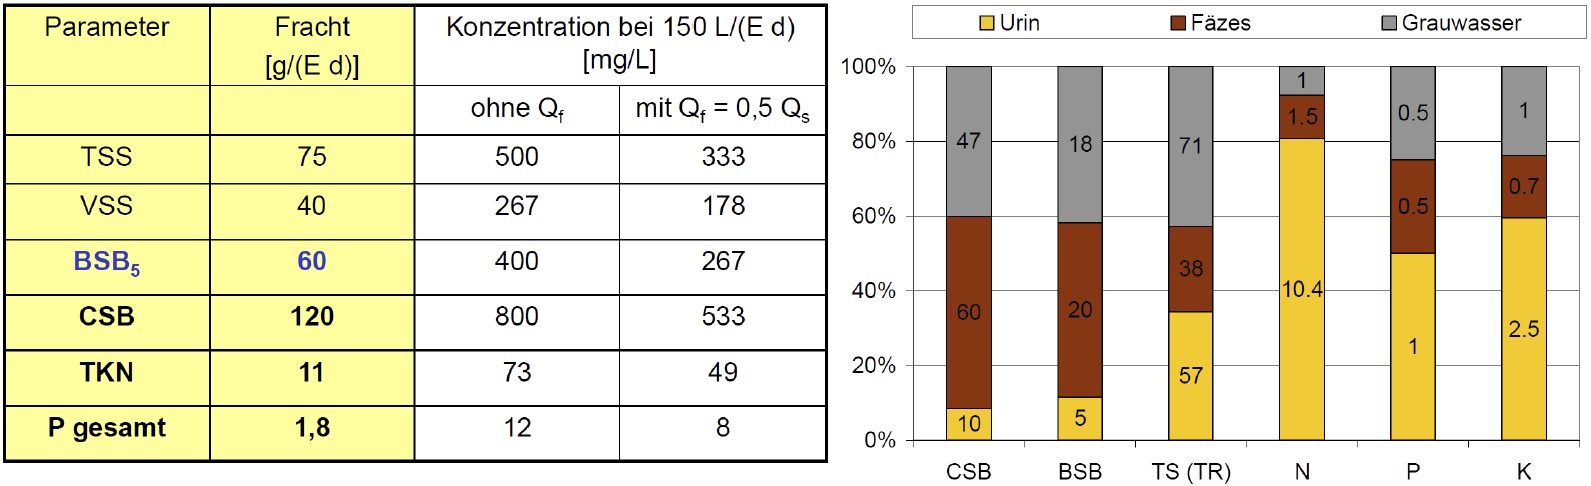
\includegraphics[width=0.8\textwidth]{images/schmutzfracht}
\end{center}\index{Durchschnittswerte Schmutzabwasser} \index{TSS! Durchschnittswerte} \index{GUS! Durchschnittswerte} \index{BSB\textsubscript{5}! Durchschnittswerte} \index{CSB! Durchschnittswerte} \index{TKN! Durchschnittswerte}
\subsection{Regenabwasser}
Bei Regenabwasser stammt die Schmutzfracht\index{Schmutzfracht} von den Oberflächen. Die Stoffe werden bei Trockenwetter akkumuliert. Sie stammen vom Verkehr, Winterdienst, Vegetation, Baumassnahmen etc. und werden durch Wind und Strassenreinigung in Senken angesammelt. Bei Niederschlag werden die Stoffe abgetragen. Die Stoffmenge ist jedoch meist begrenzt, sodass die deponierte Menge limitierend wirkt auf den totalen Frachtaustrag\index{Frachtaustrag} in Gewässer und Boden. Es kommt zu einer sogenannten Stossbelastung. Die Stoffbelastung (CSB) ist zu Beginn des Regenereignisses sehr hoch. Im Verlauf kommt es jedoch zur Verdünnung infolge Frachtanstieg und steigender Abflussmenge. Diese Stossbelastung\index{Stossbelastung}, oft auch \index{First-Flush}\glqq First-Flush\grqq genannt, ist oft verbunden mit der hydraulischen Stossbelastung des Vorfluters. Bei Starkregen kann bis zu 80 mal mehr Niederschlagswasser als Schmutzwasser kommen. Im Kanalisationsnetz puffern\index{Rückhaltebecken} Rückhaltebecken und \index{Retention}Retentionen den \glqq First-Flush\grqq im Gewässer.
\section{Diffuse Belastung bei Regenwetter}
\index{Diffuse Belastung}Viele Oberflächen sind in Kontakt mit Regenwasser. Dazu gehören Metalldächer und -fassaden, Kunstoff-/Bitumendächer, WDVS-Fassaden, Flughäfen, Eisenbahn, Parkplätze, Strassen, Drainagen etc. Diese verschiedensten Materialien enthalten zum Teil Schadstoffe. Flüssigkunststoffe enthalten zum Beispiel hormonaktive Stoffe und Cyanide, deshalb immer die Merkblätter lesen und Vollschutz tragen. In Baustoffen kommen oft Biozide, Durchwurzelungschutz, UV-Filter, Flammschutzmittel, Weichmacher, Stabilisatoren für Kunsstoffe, Korrosionsschutzmittel (organisch) und viele weitere zum Einsatz. Durch Auswaschungen können diese Stoffe in Gewässer eingetragen werden. Alle Bauprodukte müssen deshalb\index{CE Zertifikat} CE zertifiziert sein. Dieses Zertifikat wird jedoch nur selten nachgefragt. In der Schweiz sind zudem folgende Verordnungen relevant:
\begin{itemize}
\item Biozidprodukteverordnung (VBP)\index{Biozidprodukteverordnung (VBP)}: 22 Produktarten, Biozidprodukte (Risiko bewerten) und behandelte Waren (Risiko kennzeichnen)
\item Bauprodukteverordnung (BauPV)\index{Bauprodukteverordnung (BauPV)}: Bewertung und CE-Kennzeichnung vom Bauprodukt (Leistungserklärung)
\item Chemikalien-Risikoreduktions-Verordnung (ChemRRV)\index{Chemikalien-Risikoreduktions-Verordnung (ChemRRV)}
\end{itemize}
\paragraph{Biozide in Bauprodukten} Bauprodukte mit\index{Biozide} Bioziden müssen zugelassen sein und eine Gefahrenkennzeichnung aufweisen. Die verwendeten Wirkstoffe müssen für die betreffende Produktart notifiziert oder gelistet sein. Zulassungen erfolgen nur durch die Anmeldestelle Chemikalien. Produktarten für\index{Biozide! Produktarten} Biozidprodukte für Beschichtungen: PA6: Topf-Konservierungsmittel, PA7: Beschichtungsschutzmittel, PA8: Holzschutzmittel (Biozidprodukte) und PA9: Schutzmittel für Mauerwerk. Häufig werden Biozide in Putz und Farbe verwendet um den Algen- und Pilzbefall zu verhindern, da ansonsten die Beschichtung zerstört würde. Der Massgebende Punkt für die Konzentration ist das Gewässer. Das heisst, das bis zum Gewässer eine genügend grosse Menge Wasser zugeführt werden muss, damit die Verdünnung ausreichend ist um die gesetzlichen Anforderungen zu erfüllen. Mögliche Massnahmen sind umweltverträglichere Produkte. Dabei können die Stoffe verkapselt werden, was zu 5-10 mal geringeren Auswaschungen führt (80\% der Produkte). Oder\index{Biozide! schnell abbaubare Biozide} schnell abbaubare Biozide wie zum Beispiel OIT oder DCOIT verwenden. Weiter können auch retentionsstarke Bindemittel Produkte umweltverträglicher machen. Eine zweite Massnahme zielt auf das Umweltverhalten ab. Dabei sollen mittels eine Umweltetikette die Produkte kategorisiert werden. A und B heisst dann, dass keine Biozide für den Filmschutz eingesetzt werden. Klasse C bedeutet, dass verkapselte und schnell abbaubare Biozide verwendet werden. Natürlich kann auch eine Nachhaltige Architektur mit Materialsubstitution, Ersatz von Putz und Farbe durch rein mineralische Stoffe wie Klinker, Stein etc., eine gute Massnahme darstellen. Dies ist jedoch auch abhängig von den Kosten, der Ästhetik und so weiter.
\paragraph{Produktverbesserungen in Bitumen} Bitumendichtungsbahnen (WF) enthalten gegen Durchwurzelung einen Ester von Mecoprop oder MCPA. Pro Quadratmeter enthalten diese Bahnen zirka 10-20 g Mecoprop als Ethylhexylester und Octylester. Dieser wird durch Hydrolyse und Auswaschung bei Regenwetter freigesetzt. Möglich Massnahmen sind Bitumenbahnen mit weniger MCPP oder mit \glqq besseren\grqq \index{MCPP-Ester}MCPP-Estern. Zwischen 1995 und 2010 konnte so die\index{Mecoprop} Mecoprop-Menge von 1.2\% auf 0.35\% im Bitumen reduziert werden. Alternativen sind Ethylhexylesterund n-Octylester. Weiter können die Bitumenbahnen in Belastungsklassen eingeteilt werden, welche mittels Auswaschtests und Extrapolation über 30 Jahre Lebensdauer ermittelt wurden. Hoch: Bahnen z.B. mit Polyglykolester $>$200 mg/m\textsuperscript{2} MCPP; Mittel: heutige Bahnen 10 bis 200 mg/m\textsuperscript{2} MCPP (Regelfall); Gering: Einige Produkte $<$10 mg/m\textsuperscript{2} MCPP. Der Behandlungsbedarf der Abwässer von solchen Oberflächen orientiert sich an den Belastungsklassen. Hohe Belastung: in Kläranlage oder mit hoch wirksamen Substrat; Mittlere Belastung (Regelfall): Behandlung mit Boden oder Substrat; Geringe Belastung: ohne Behandlung einleiten oder versickern. 
\paragraph{Betonzusatzmittel}\index{Betonzusatzmittel} Sie werden im Betonbau eingesetzt und können durch \index{Auswaschung}Auswaschungen in das Gewässer gelangen. Beispiele für Zusatzmittel sind: \begin{itemize}
\item Verflüssiger,Fließmittel, z.B. Lignin-, Naphtalin-, Melaminsulfonate
\item Verzögerer, z.B. Phosphatverbindungen, Formiate, Fluoride
\item Entschäumer, z.B. Tri-iso-butylphosphat, ethoxylierte Alkohole
\item Schaumbildner, z.B. Aminoxide, Polyglykolsulfate
\item Biozide, z.B. Quartäre Ammoniumverbindungen, CMI/MI, Bronopol
\item Mikrohohlkugeln, Schwindreduzierer, Luftporenbildner etc.
\end{itemize}
Im Stahlhochbau und Stahlwasserbau kommen vor allem Epoxyharze zum Einsatz. Diese enthalten BPA, welches auswaschbar und massgeblich für den\index{Ökotox} Ökotox der Epoxydharze ist.
\paragraph{Metallflächen} In der Architektur werden häufig Metalloberflächen geplant. Durch Auswaschungen gelangen die Metalle in die Umwelt. Vor allem Kupferoberflächen und Zinkverkleidungen sind diesbezüglich problematisch. Besser alternative Metallabdeckungen gemäss KBOB verwenden oder beschichtete Metallflächen einsetzten. Bezüglich der Beschichtungen, muss diese jedoch über die ganze Lebensdauer stabil sein. Solche Nachweise fehlen heute in der Schweiz noch, werden aber gefordert und gewünscht.
\paragraph{Belastungsklassen Dächer} \index{Belastungsklassen}Die neue VSA Richtlinie Abwasserbewirtschaftung bei Regenwetter (2019)\index{Richtlinie Abwasserbewirtschaftung bei Regenwetter} sieht verschiedene Belastungsklassen vor:
\begin{center}
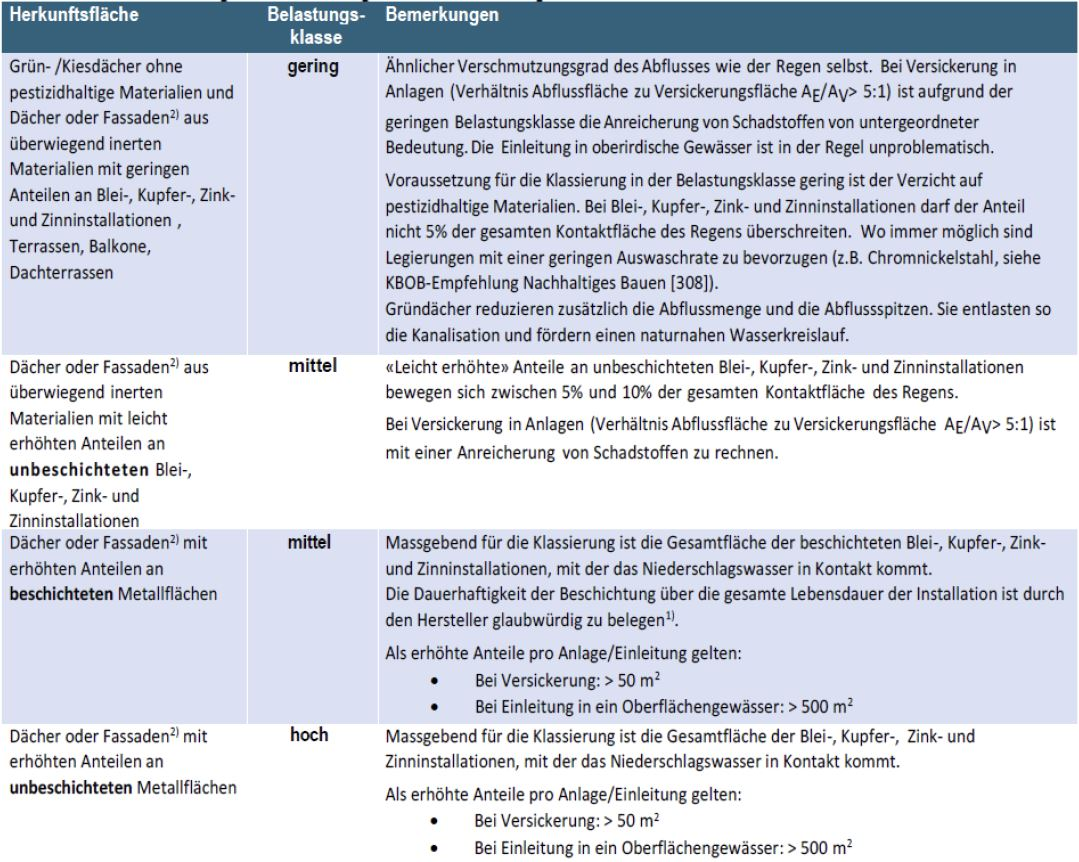
\includegraphics[width=0.9\textwidth]{images/belastungsklassen}
\end{center}
Solche Tabellen gibt es auch für Strassen, Plätze und so weiter. Die Belastungsklassierung hat sich gegenüber der Alten Richtlinie nichts geändert: \index{Belastungsklassierung}
\begin{center}
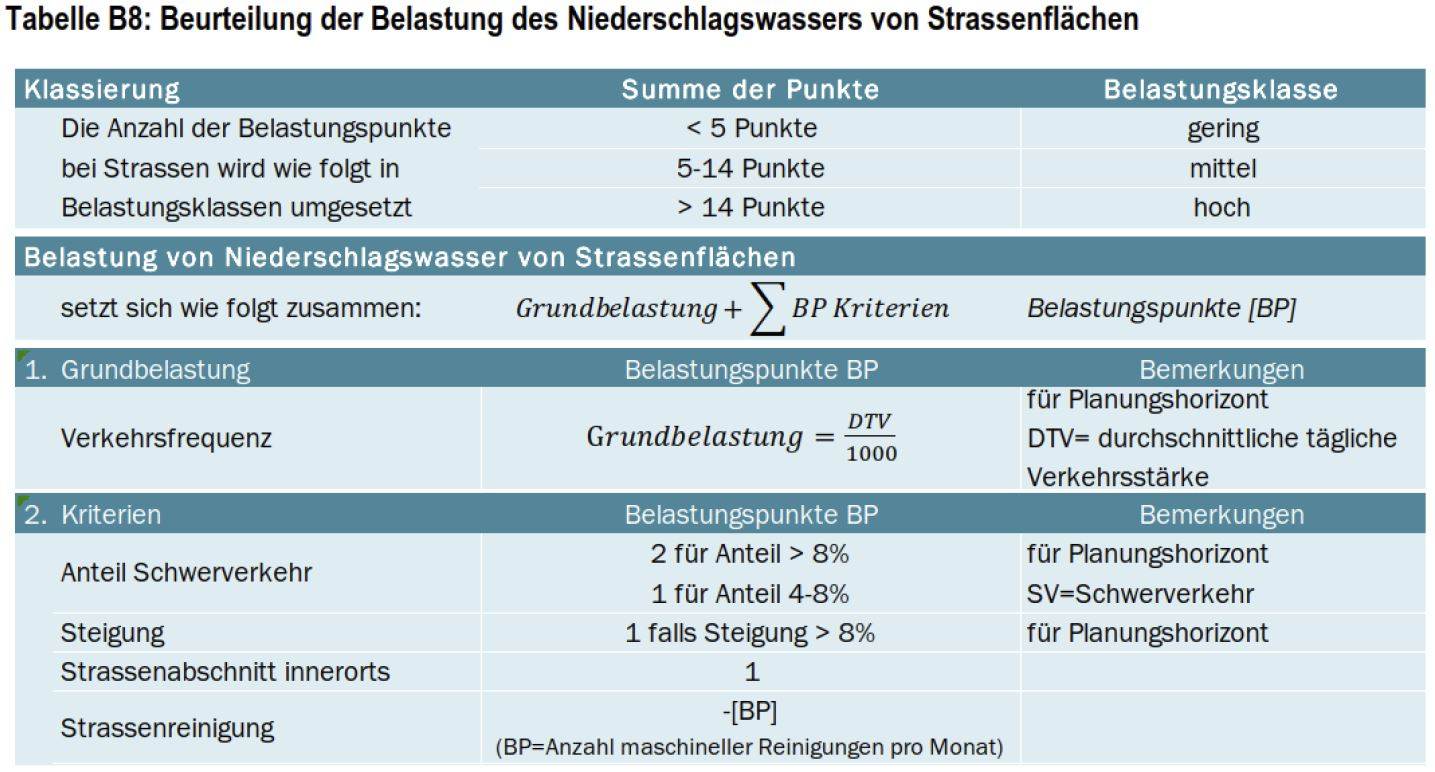
\includegraphics[width=0.8\textwidth]{images/belastungsklassierung}
\end{center}\par \clearpage
\subsection{Diffuser Eintrag über das Trennsystem} \index{Diffuser Eintrag über das Trennsystem}
Der Eintrag von Mikroverunreinigungen geschieht durch Versickerung, Meteorwasser oder Regenüberläufe. Im Bereich der Siedlungen und Liegenschaften gibt es hohe Oberflächenabflüsse, da der Versiegelungsgrad sehr hoch ist und eine geringe Abflussretention stattfindet. Die Abflussbeiwerte liegen zum Teil über 0.8. Selten steht eine Wasserbewirtschaftung im Vordergrund. Vielmehr soll das Wasser möglichst schnell entsorgt werden. Die geschieht meist über Drainagen oder Versickerungen. Zudem wird das Wasser dann unkontrolliert (diffus) in eine Vorflut geleitet. So kann nicht gewährleistet werden, dass das Wasser bei der Einleitung nicht verschmutzt ist.
\subsection{Behandlung von Regenabwasser} \index{Behandlung von Regenabwasser}
Folgende Übersicht zeigt das Behandlungsangebot\index{Behandlungsangebot} für verschmutztes Regenabwasser:
\begin{center}
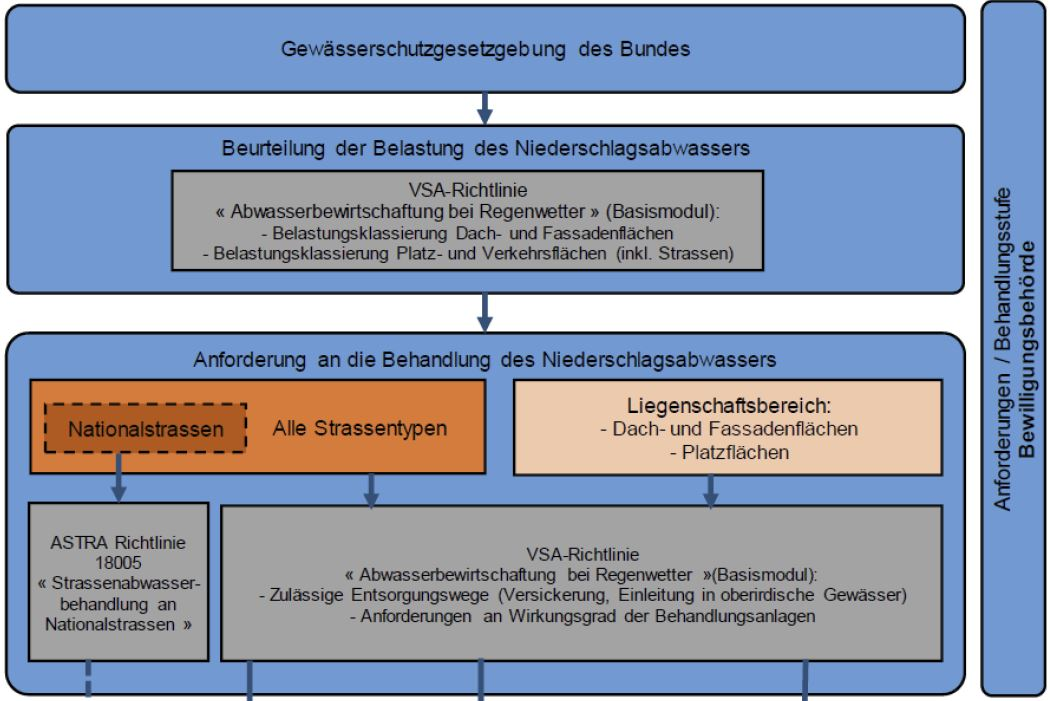
\includegraphics[width=0.8\textwidth]{images/behandlungsangebot}
\end{center}\par
Vor einer Einleitung oder \index{Versickerung}Versickerung muss jedoch erst die Zulässigkeit geprüft werden. Dies geschieht mit Hilfe der VSA Richtlinie. Dabei wird unterschieden zwischen Versickerung und Einleitung in ein Oberflächengewässer. Bei der Einleitung in ein Oberflächengewässer müssen sowohl Anforderungen an die Stoffmenge, als auch hydraulische Faktoren erfüllt sein.
\begin{center}
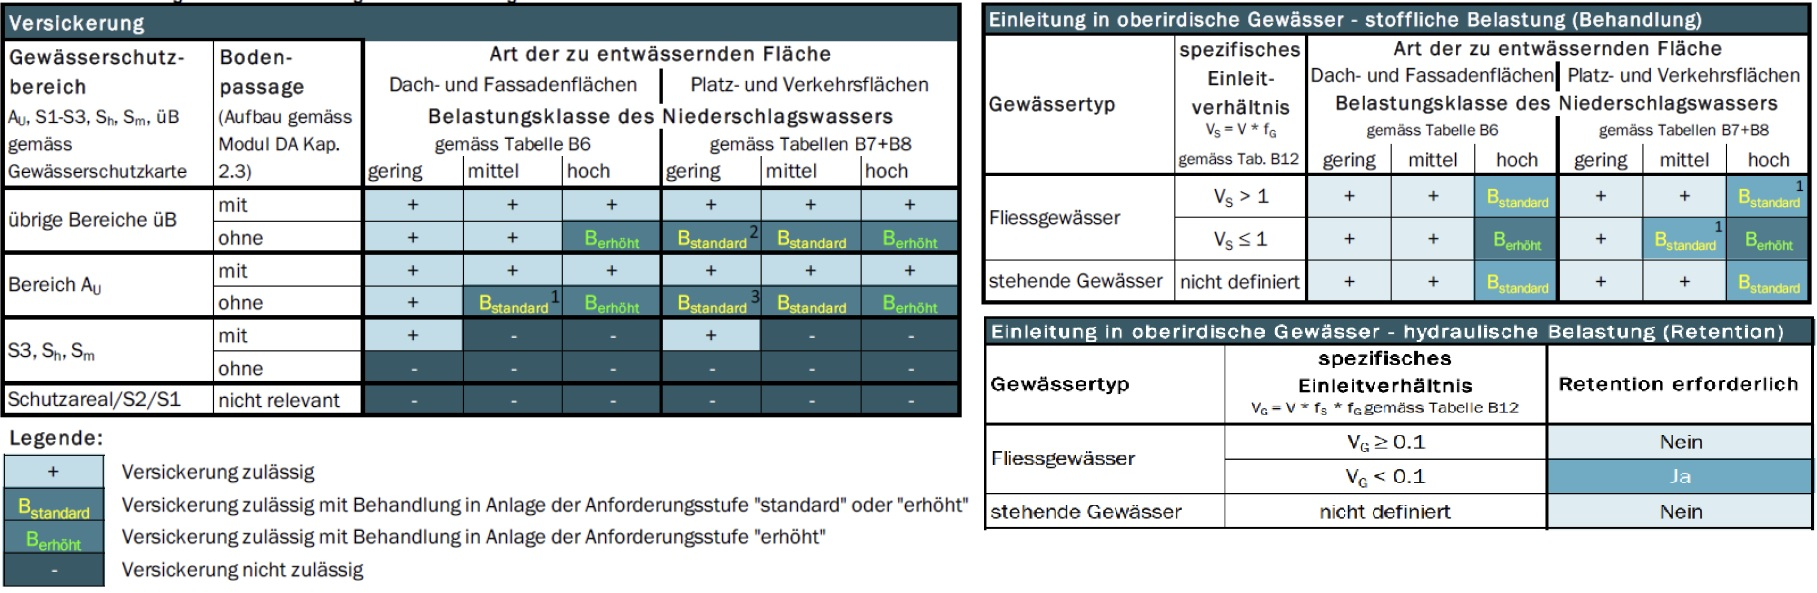
\includegraphics[width=\textwidth]{images/zulaessigkeit}
\end{center}\par
Diese Beurteilung bezieht sich nur auf einzelne Einleitungen (Einzeleinleitungen). Die Bagatellgrenze liegt bei 20 Liter pro Sekunde. Die Betrachtung der Wirkung von mehreren Einleitstellen findet auf übergeordneter Ebene (GEP) mit STORM statt. Für die Behandlung von Regenabwasser gibt es verschiedene Möglichkeiten. Diese werden im folgenden kurz vorgestellt. \clearpage
\paragraph{Naturnahe Behandlungsanlagen}\index{Versickerungsanlagen} Die Behandlung erfolgt durch  kontrollierte Akkumulation in einer Sickerschicht\begin{wrapfigure}{f}{7cm} 
  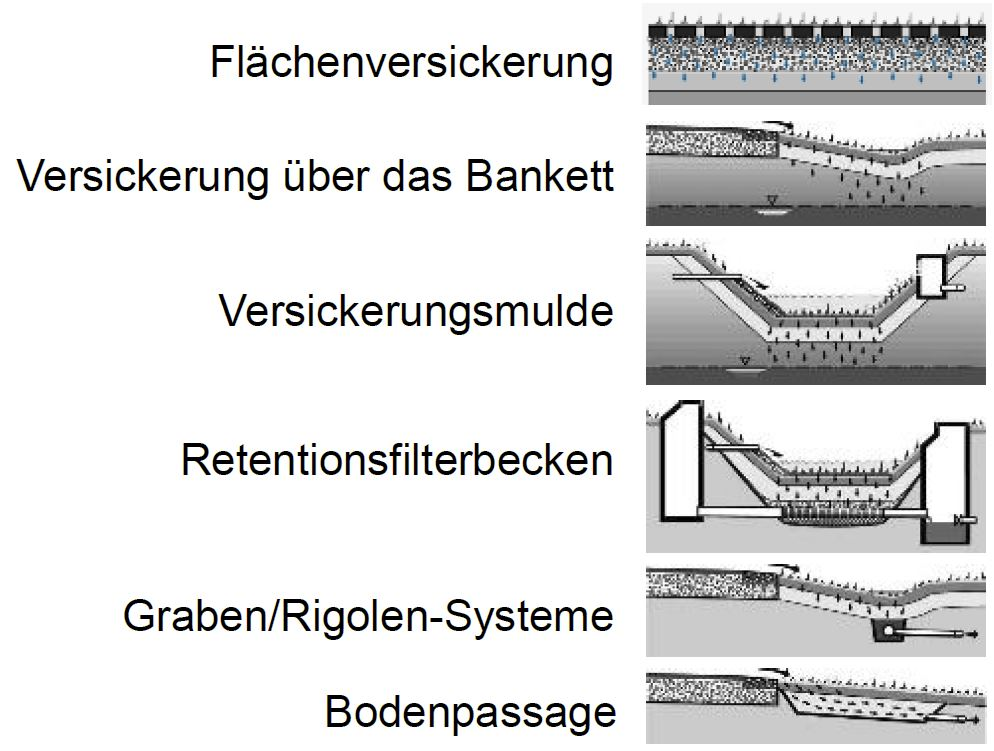
\includegraphics[width=.45\textwidth]{images/versickerungsanlagen}
\end{wrapfigure} (Schadstoffsenke)\index{Schadstoffsenke}. Solche Anlagen weisen eine hohe Leistung bei einer \index{Flächenversickerung}Flächenversickerung auf (GUS, SM-Adsorption). Es besteht jedoch die Gefahr von \index{Kolmation}Kolmation und innerer Suffosion\index{innere Suffosion}. Mögliche Formen von Versickerungsanlagen sind in der nebenstehenden Abbildung aufgeführt. Natürlich haben auch solche Anlagen Limitierungen. So wird das Bodengefüge durch Umlagerungen zerstört werden und es kommt zur Suffosion. Bepflanzungen stabilisieren hier das Bodengefüge und sichern die Durchlässigkeit. In bindigen Böden kommt es durch präferentiellen Transport zu schnellen Stoffverlagerungen. Zudem weisen nur wenige natürliche Böden die erforderliche Wasserleitfähigkeit\index{k\textsubscript{f}} ($k_f > 10^{-5} m/s$) und Adsorptionskapazität (Ton $>$ 10\%) auf. Die Anforderungen nach VSA sind für den Oberboden (A-Horizont; 30cm): pH grösser als 6.5, Humusgehalt über 4\% und einen Tongehalt zwischen 8 und 30\%. Für den Unterboden (B-Horizont; 50cm) einen pH Wert über 5.5 und einen Humusgehalt kleiner als 1\% und einen Tongehalt zwischen 10 und 35\%. 
\paragraph{Dezentrale Kompaktanlagen} Solche Anlagen bestehen aus einem oder mehreren Schächten und können für die Anforderungen der Versickerung und Direkteinleitung ausgelegt werden. Die Leistungsprüfung erfolgt mit Labortests mit Adsorbermaterialien\index{Adsorber} und Anlagentests an zwei Standorten. Mit den Analgen können GUS, Kupfer, Zink, Mecoprop und Diuron zurückgehalten werden. Anlagen mit über 70\% Stoffrückhalt werden durch den VSA empfohlen.
\subsection{Strassenwasserbehandlung}
\paragraph{Belastungssituation} Durch die Schweiz führen 1'900 km Autobahn, 18'000 km Kantonsstrassen und 50'000 km Gemeindestrassen. An den Autobahnen gibt es rund 1'000 Einleitstellen in Gewässer. Rund 14'000 Tonnen pro Jahr ungelöste Stoffe (GUS) fallen an, welche zwischen 10 und 60\% der Gesamtemission ausmachen. Es bestehen Bestrebungen nur den hydraulischen Wirkungsgrad und den Rückhalt von GUS als Leistungsmerkmal zu überwachen. Der Grund ist die Annahme, dass 50-70\% der Schwermetalle gebunden vorliegen. Gelöste Schadstoffe werden so jedoch übersehen. Im Strassenabwasser kommen unter anderem\index{PAK} PAK's, BPA\index{BPA}, OP\index{OP}, NP\index{NP}, DEHP\index{DEHP} vor. Sie sind rund 60-80\% Frachtanteil an diffusen Einträgen. 
\paragraph{SABA's} Die Strassenabwässer der Autobahnen werden in Strassenabwasserbehandlungsanlagen (SABA)\index{SABA}\index{Strassenabwasserbehandlungsanlage} aufbereitet. Die Bodenfilter\index{Bodenfilter} einer SABA benötigen rund ein Jahr, bis er einsatzfähig ist. Die Oberflächenentwässerung der Strasse erfolgt über Schlammsammler. In diesen setzt sich der Sand und Schlamm unten ab. Durch einen Tauchbogen wird verhinder, dass Öle abfliessen. Die SABA selber hat meist eine Vorabscheidung für GUS\index{GUS} in Form eines Absetzbeckens. Vor der Einleitung des Wassers in den Bach, wird das Wasser durch einen bepflanzten Sandfilter geleitet. In einigen SABA's kommen auch Trommelfilter zum Einsatz. Die hydraulische Leistung liegt bei 33'000 m\textsuperscript{3}/ Jahr. Die Partikelabscheidung erfolgt durch Scheibenfilter. Die Kosten dieser Anlage liegen bei 3.5 Mio. CHF.  
\paragraph{Strassenwasserbehandlung} Auch auf privaten Plätzen muss das Wasser von Plätzen und Strassen behandelt werden. Vielfach werden Rinnen eingesetzt um Platzwasser zu sammeln, diese können aber auch direkt als Filter eingesetzt werden. Regenwasser fliesst der offenen oder mit einem befahrbaren Gitterrostabgedeckten Mulde / Rinne oberflächig zu. Reinigung erfolgt während der Passage durch ein spezielles Substratmit kf-Wert von $9 \cdot 10^{-4}m/s$. Die Rinne hat damit die Funktion einer Muldenversickerung. 
\paragraph{Dezentrale Kompaktanlagen} Dezentrale\index{dezentrale Kompaktanlagen} technische Behandlungsanlagen (3P Technik, Rehau,Mall, Funke etc.) scheiden die GUS's ab. Wirbelabscheider werden eingesetzt zur Sedimentation von Partikeln. Durch unterschiedliche Filtermaterialien je nach Belastung mit Wirkungsgraden für GUS, MKW, Cu, Zn im Mittel von bis zu 90\%. 
\subsection{Liegenschaftsentwässerung}
Auch in der Liegenschaftsentwässerung können Schadstoffe nachgewiesen werden. Am Beispiel Volketswil wurden diesbezüglich bereits Untersuchungen vorgenommen. Dazu wurden Regenwasserkanäle instrumentiert um die Belastungen zu messen. So konnten Terbutryn aus Fassaden, \index{Mecoprop}Mecoprop aus Bitumenbahnen und \index{Glyphosat}Glyphosat gegen Unkraut (PSM) nachgewiesen werden. Für Wohnüberbauungen können heute dezentrale Regenwasserbehandlungen in Frage kommen um solche Stoffe zu binden. Dazu wird das Wasser in einem Retentionsbecken aufgefangen, durch einen \index{Adsorber}Adsorber geleitet und anschliessend versickert. Dies ist eine sogenannte\index{Nachgeschaltete Massnahme} Nachgeschaltete Massnahme. Diese erfordern ein gutes Monitoring und eine ausgeklügelte Regelung. Sie bieten dafür einen breiten Stoffrückhalt durch Mischadsorber mit granulierter Aktivkohle (40cm Schichthöhe). So können Carbendazim, Diuron und Kupfer (80\%), Terbutryn und Zink (50-80\%) und MCPP und DEET (30-70\%) zurückgehalten werden. Ein weiterer Vorteil ist, dass die Durchlässigkeit auch nach über vier Jahren nicht abnimmt.
\section{Kommunale Kläranlagen}
\paragraph{Mischwasserbehandlung}\index{Mischabwasserbehandlung}\index{Kommunale Kläranlagen} Eine ARA reinigt Mischwasser bis zur doppelten Abwassermenge, die bei Tagesspitzen an einem Trockenwettertag anfällt ($Q_{ARA} \approx 2 \cdot Q_{TW}$). Mittlere Regen füllen die Regenüberlaufbecken im Netz. Stärkere und längere Regen bringen soviel Wasser, dass die Regenbecken überlaufen und Mischwasser entlastet werden muss. Bei extrem intensiven Regen ($r > r_{krit}$) wird Mischwasser am Regenüberlaufbecken vorbeigeleitet oder in Hochwasserentlastungsanlagen direkt in die Vorflut entlastet.\index{Schema Kanalisation} \index{Regenintensität Schweizer Mittelland}
\begin{center}
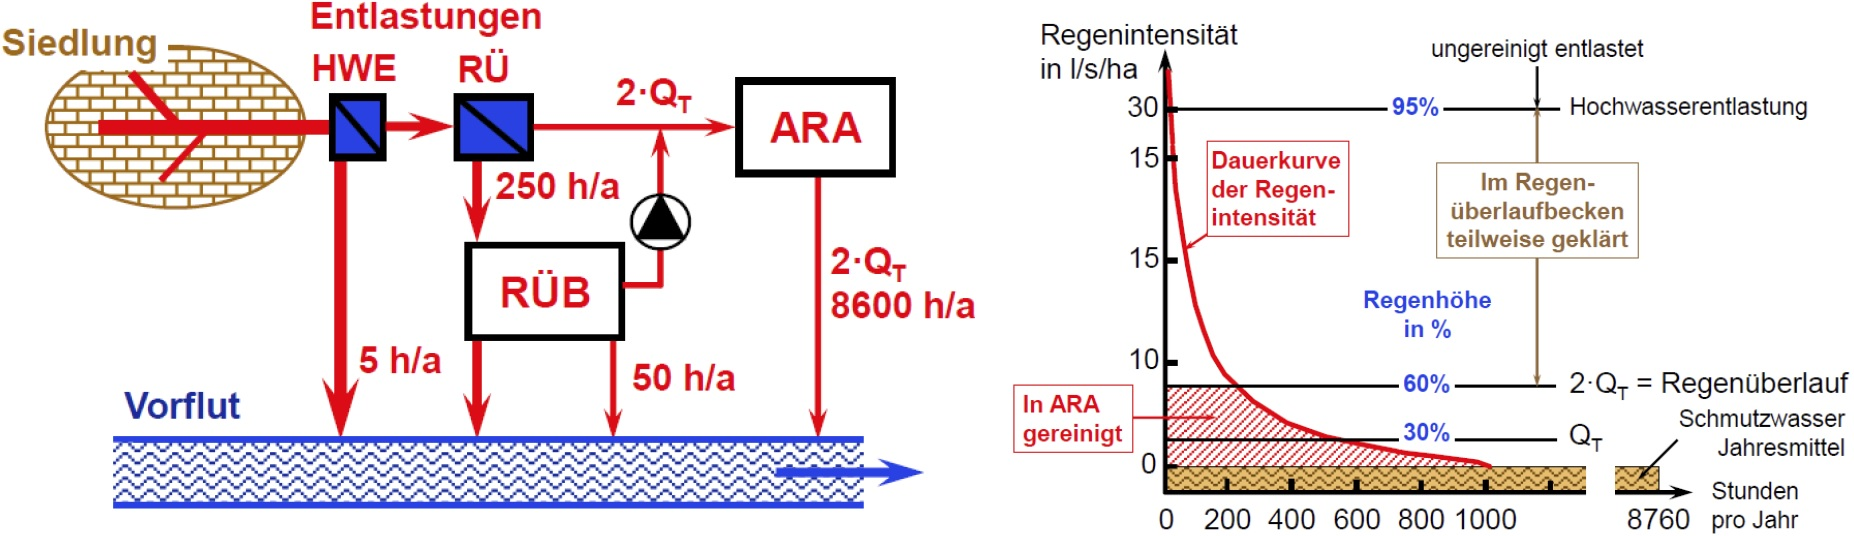
\includegraphics[width=\textwidth]{images/schemakanalisation}
\end{center}
Obige Abbildung zeigt zudem die Summenhäufigkeitsverteilung der Regenintensität im Schweizerischen Mittelland und den typischen Abwasseranfall bei Trockenwetter. Die Entlastungen in Bäche sollten durch Betriebsoptimierungen stark reduziert werden, da sonst Schadstoffe in die Gewässer gelangen.
\paragraph{Kommunale Abwasserreinigungsanlagen} Die Dimensionierungsgrösse für Kläranlagen ist der Einwohnerwert (EW).\index{Einwohnerwert} Dazu gehört zum Beispiel der BSB\textsubscript{5} pro Einwohner und Tag. Folgende Tabelle zeigt für die Schweiz typische Werte:
\begin{table}[h]
\small
\begin{tabularx}{1\textwidth}{X C{0.2\textwidth} C{0.2\textwidth} C{0.2\textwidth}}
\toprule
Stoff & Rohabwasser & \multicolumn{2}{c}{Vorgeklärtes Abwasser} \\ 
 &  & \multicolumn{2}{c}{Aufenthaltszeit im Vorklärbecken} \\ 
 & g/EW/d & 0.5 - 1.0 h & 1.5 - 2.0 h \\ 
\midrule 
BSB\textsubscript{5} & 60 & 45 & 40\\
CSB & 120 & 90 & 80\\
TSS / GUS& 70 & 35 & 25\\
TKN & 11 & 10  &10\\
P\textsubscript{tot} & 1.8 & 1.6 & 1.6\\
\midrule
\end{tabularx} 
\end{table}\par
Multipliziert man den BSB\textsubscript{5}-Wert mit dem Einwohnerwert (Anzahle Einwohner), erhält man den Sauerstoffbedarf im Betrieb. \index{Sauerstoffbedarf im Betrieb}
\paragraph{Stufen der Abwasserreinigung} \index{Stufen der Abwasserreinigung}
\begin{enumerate}
\item Stufe: Mechanische Reinigung
\begin{itemize}
\item Rechen: Entfernung von groben Feststoffen
\item Sandfang: Absetzen von mineralischen Schmutzstoffen (Sand)
\item Fettfang: Ölabscheider
\item Vorklärbecken: Absetzen von biologischen Schmutzstoffen
\end{itemize}
\item Stufe: Biologische Reinigung
\begin{itemize}
\item Gelöste organische Verbindungen werden zu Biomasse und CO\textsubscript{2} umgesetzt(oxidiert) und Stickstoffverbindungen (Ammonium, Nitrat) entfernt
\item Abzug von Schlamm, sogenanntem \glqq Überschussschlamm\grqq
\end{itemize}
\item Stufe: Chemische Nachbehandlung
\begin{itemize}
\item Fällung von Phosphaten mit Eisen- oder Aluminiumsalzen
\item Kein spezielles Becken, sondern auf die Anlage \glqq aufgesetzt\grqq
\end{itemize}
\item Stufe: Mikroverunreinigungen
\end{enumerate}
Die Eliminationsleistung\index{Eliminationsleistung} über die drei (vier) Stufen ist für verschiedene Stoffe unterschiedlich. Die Filtration gehört zur physikalischen Stufe\index{Physikalische Stufe} einer ARA.
\begin{multicols}{2}
Hohe Elimination
\begin{itemize}
 \item BSB\textsubscript{5}: 93\%
 \item GUS: 98\%
 \item Phosphat: 95\%
 \item Ammonium-N.: 90\%
\end{itemize}
Geringe Elimination
\begin{itemize}
 \item Organische Mikroverunreinigungen, z.B. Pestizide, Pharmaka, Industriechemikalien
 \item Salze ($SO_4^{2-}, Cl^-$)
 \item Einige Schwermetalle
\end{itemize}
\end{multicols} 
In Zukunft kommt noch eine weitere vierte Stufe für Mikroverunreinigungen hinzu. Diese wird zum Teil schon eingesetzt. In dieser Stufe erfolgt der Abbau durch Ozonung (oder andere Oxidationsprozesse), durch Adsorption an Aktivkohle (Pulverkohle, granulierte Aktovkohle) oder durch Membranfiltration (Mikrofiltration mit Pulverkohle, Ultra-oder Nanofiltration).
\begin{center}
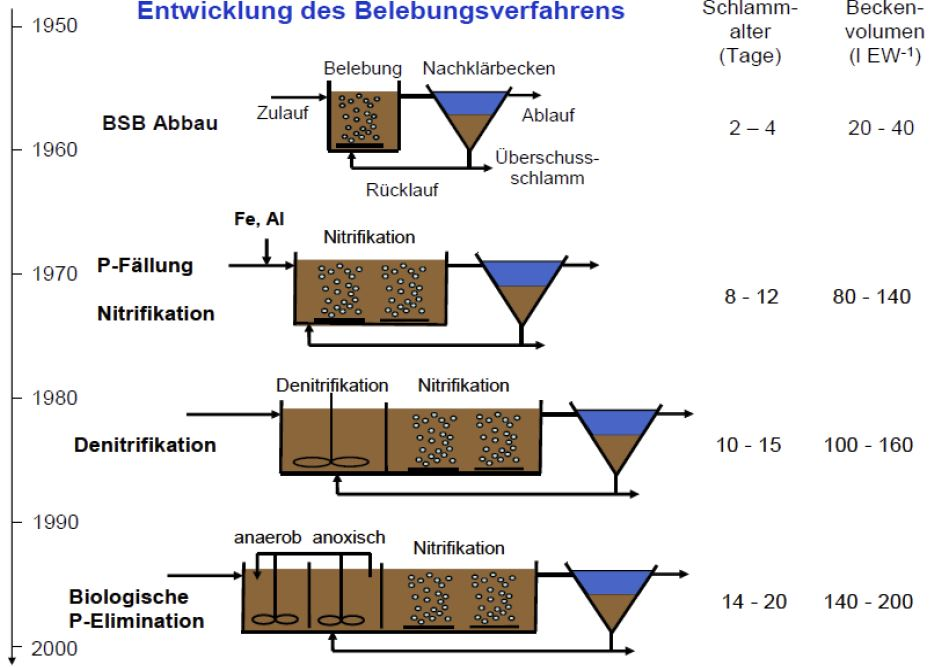
\includegraphics[width=0.7\textwidth]{images/entwicklungara}
\end{center}
\subsection{1. Stufe: Mechanische Reinigung} \index{Mechanische Reinigung} \index{1. Stufe}
Zur Mechanischen Reinigung gehören folgende Stufen: Rechen, Sand-/Fettfang und Vorklärung. Folgende Abbildung zeigt eine typische Schweizer ARA:
\begin{center}
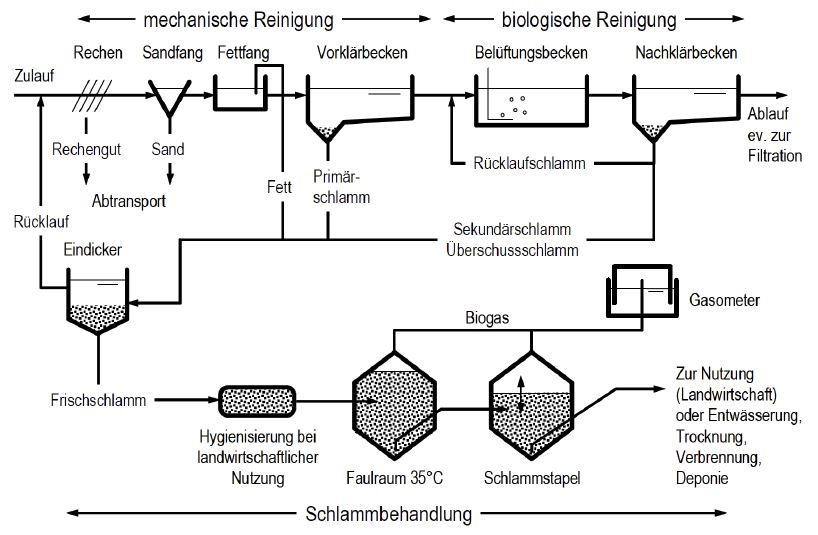
\includegraphics[width=0.7\textwidth]{images/ARA}
\end{center}\index{Schema ARA}
\paragraph{Rechen}\index{Rechen} Das Ziel des Rechens ist es, die ARA vor Verstopfungen zu schützen. Weiter hält er Plastikteilchen zurück, damit diese nicht in den Klärschlamm gelangen. Die Aufenthaltszeit beträgt zirka 10 Sekunden. Grobrechen haben Durchlässe mit einer Breite von 30-60mm. Feinrechen haben Durchlässe mit Abständen von 6-30mm, zum\begin{wrapfigure}{f}{7cm} 
  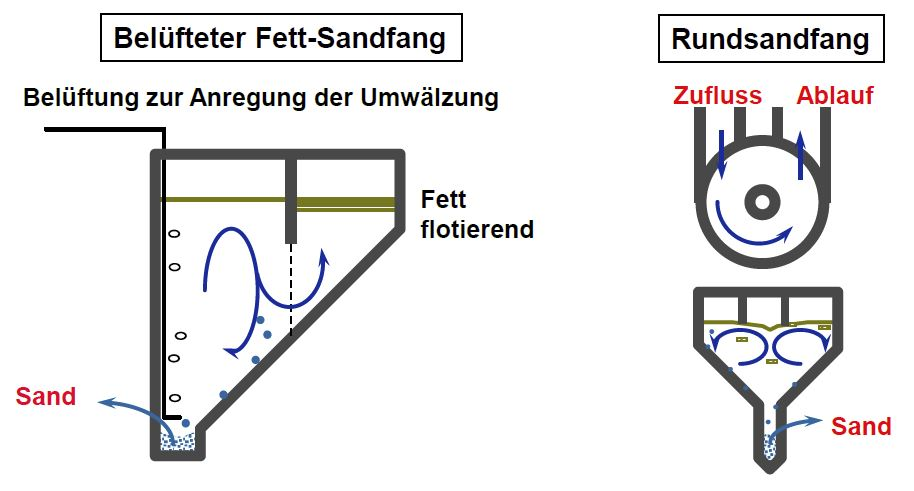
\includegraphics[width=.45\textwidth]{images/sandfang}
\end{wrapfigure} Teil bis hinunter zu Abständen von nur einem Millimeter. Der Anfall an Rechengut bei einem Stababstand von 5mm beträgt zirka 0.02m\textsuperscript{3}/EW/Jahr. Es gibt verschiedene Formen von Rechen: Hydraulikrechen oder Umlaufrechen. Das Rechengut wird zum Teil gewaschen und gepresst um Platz zu sparen.
\paragraph{Fett- und Sandfang (baulich integriert)}\index{Sandfang}\index{Fettfang} Ziel ist der Schutz vor Ablagerungen in Leitungen, Abrasion von Pumpen und Schutz der Schlammbehandlung. Fett muss entfernt werden, da es aufschwimmt und so zum Beispiel die Vorklärung behindert. Es wird Fett und Sand $>$ 0.1mm Durchmesser, der eine Sinkgeschwindigkeit von $v_S > 0.01 m/s (1 cm/s)$ aufweist zurückgehalten. Die Ablagerung von organischen Stoffen wird durch eine Fliessgeschwindigkeit von $v_f = 0.3 m/s$ gewährleistet. Die Aufenthaltszeit\index{Aufenthaltszeit} beträgt je nach Bauweise 2 bis 10 Minuten, wobei 10 Minuten der Regelfall ist. Im belüfteten Sandfang wird an einer Längsseite Luft eingeblasen. Dadurch bildet sich Wasserwalze, deren Geschwindigkeit auf ca. 30 cm/s eingestellt ist, so dass sich Sand absetzen kann und leichtere organische Stoffe (Kaffeesatz, Toilettenpapier etc.) in Schwebe bleiben.\paragraph{Dimensionierung Sandfang}\index{Dimensionierung Sandfang} \index{Sandfang Dimensionierung}
\begin{center}
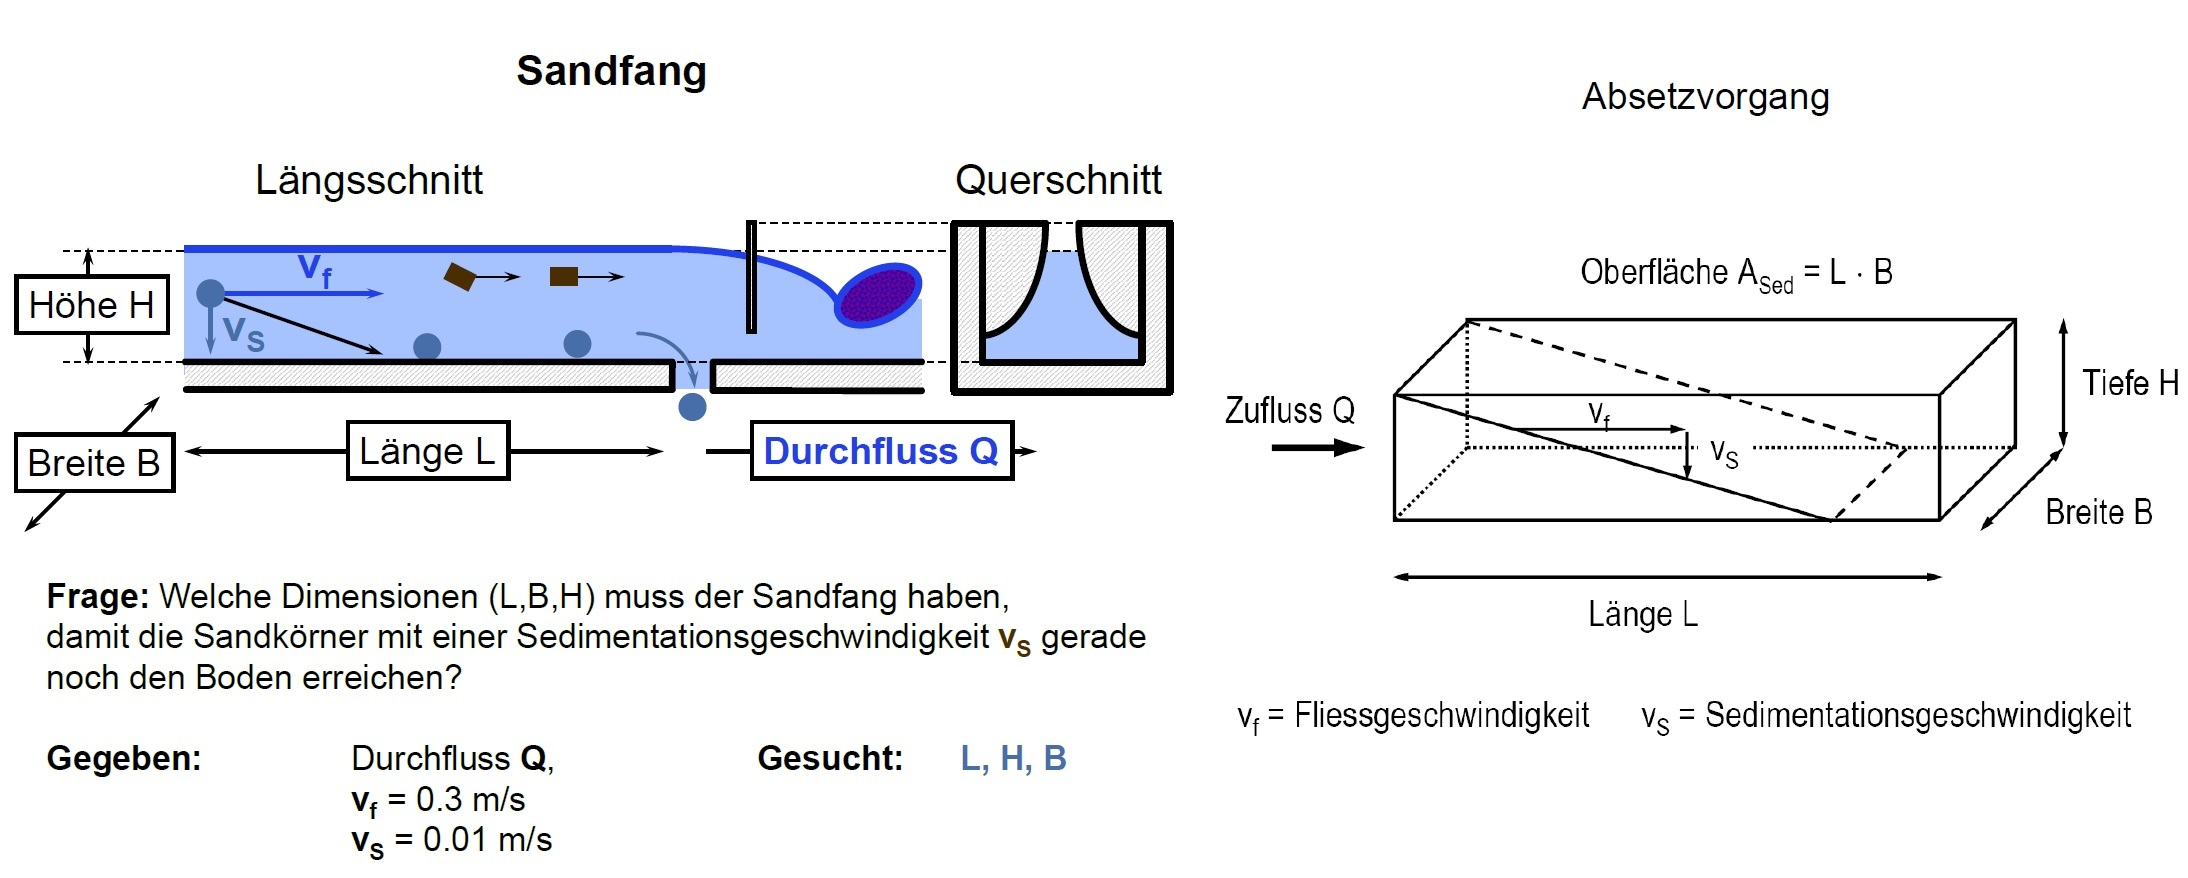
\includegraphics[width=1.0\textwidth]{images/dimensionsandfang1}
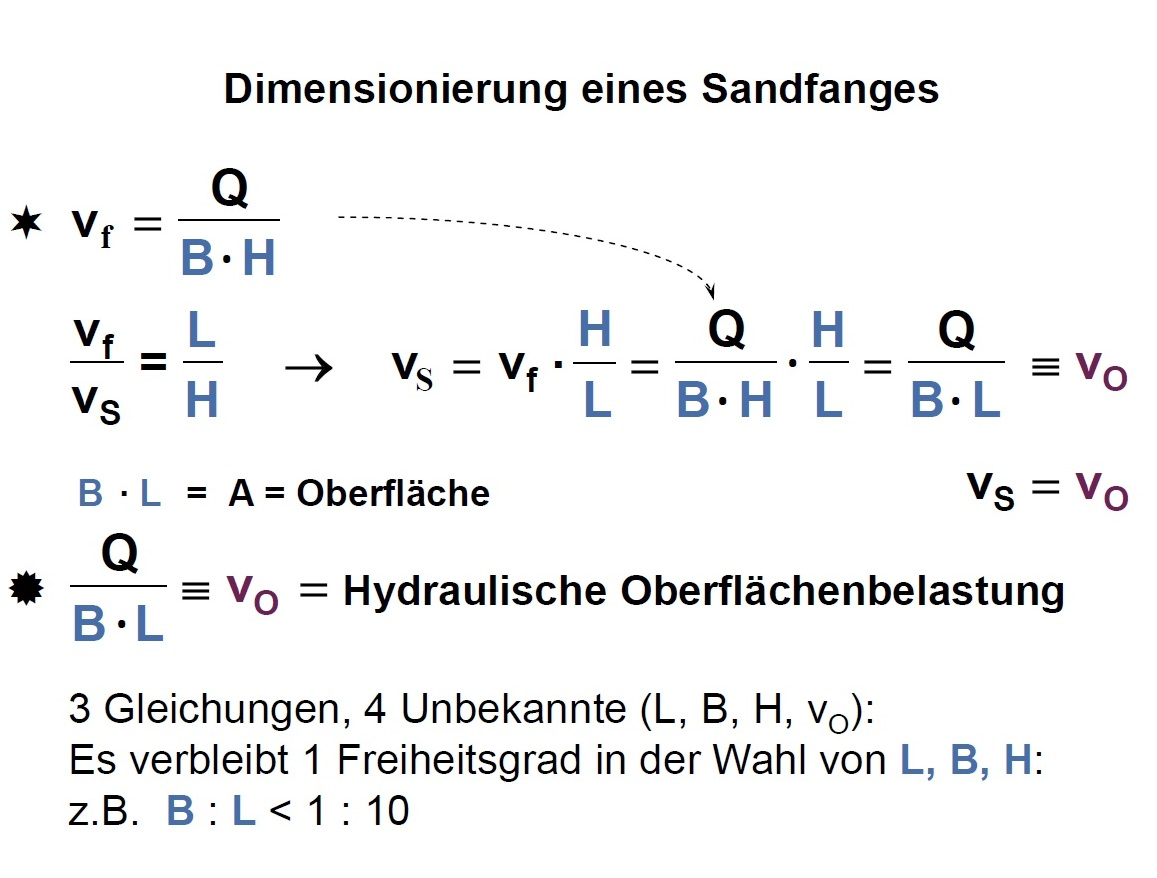
\includegraphics[width=0.5\textwidth]{images/dimensionsandfang2}
\end{center}\clearpage \begin{wrapfigure}[23]{l}{7cm} 
  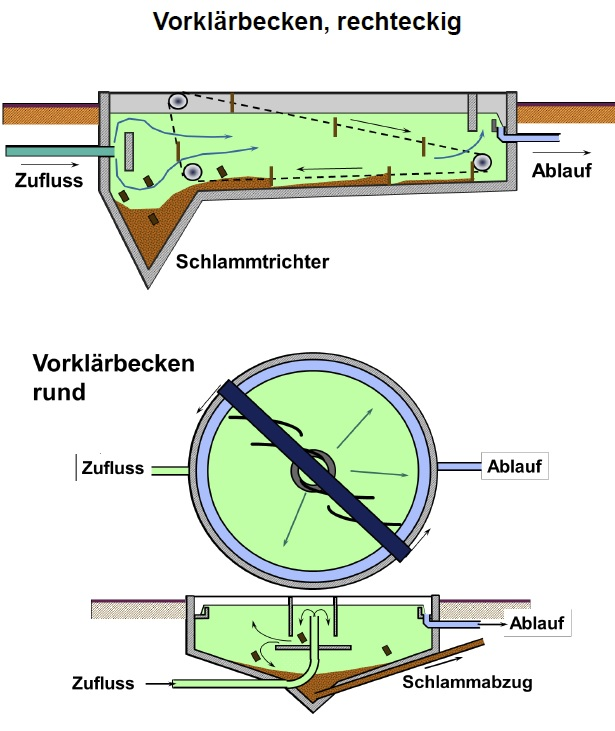
\includegraphics[width=.45\textwidth]{images/vorklaerbecken}
\end{wrapfigure}
\paragraph{Vorklärung}\index{Vorklärung} Das Ziel der Vorklärung ist das Abtrennen von absetzbaren, abfiltrierbaren und organischen Stoffen und das Aufkonzentrieren des anfallenden Schlammes. Es werden Schwebstoffe mit einer Sedimentationsgeschwindigkeit $v_S > 2 - 4 m/h$ abgetrennt. Die Hydraulische Oberflächenbelastung $v_0$ führt zu hydraulischer Aufenthaltszeit $\theta_h = \dfrac{V_{VKB}}{Q_{Zufluss}}= 0.5 – 2.0 h$ Die Organanische Fracht nimmt dabei bis zu 40\% ab (BSB\textsubscript{5}). Je nach Anlage kommen runde oder rechteckige Vorklärbecken zum Einsatz.
\paragraph{P-Elimination in der Vorklärung}\index{P-Elimination}Partikulärer Phosphor wird mit anderen Feststoffen abgeschieden. Der P-Wirkungsgrad hängt von Aufenthaltsdauer ab. Eine Aufenthaltszeit von 0.5 – 1 h reduziert Fracht von $2g P_{tot}/EW \cdot Tag$ auf $1.6g P/EW \cdot Tag$ (ca. 20\%; ATV A-131).
\subsection{2. Stufe: Biologische Reinigung}\index{Biologische Reinigung}\index{2. Stufe}
In der Biologischen Reinigung bauen Mikroorganismen organische Substanzen und Stickstoffverbindungen ab. Dies erfolgt durch die Aerobe Umwandlung zu CO\textsubscript{2} und Aufbau von \index{Biomasse}Biomasse\index{Überschussschlamm} (Überschussschlamm, ÜSS)\index{ÜSS}. Durch 1 kg BSB\textsubscript{5} wird 0.7 kg (TS) Überschussschlamm erzeugt. Dominierend sind die Bakterien. Unter dem Mikroskop sind jedoch die Protozoen auffälliger (Wimperntierchen, Wechseltierchen, Rädertierchen) \\ \\
\begin{center}
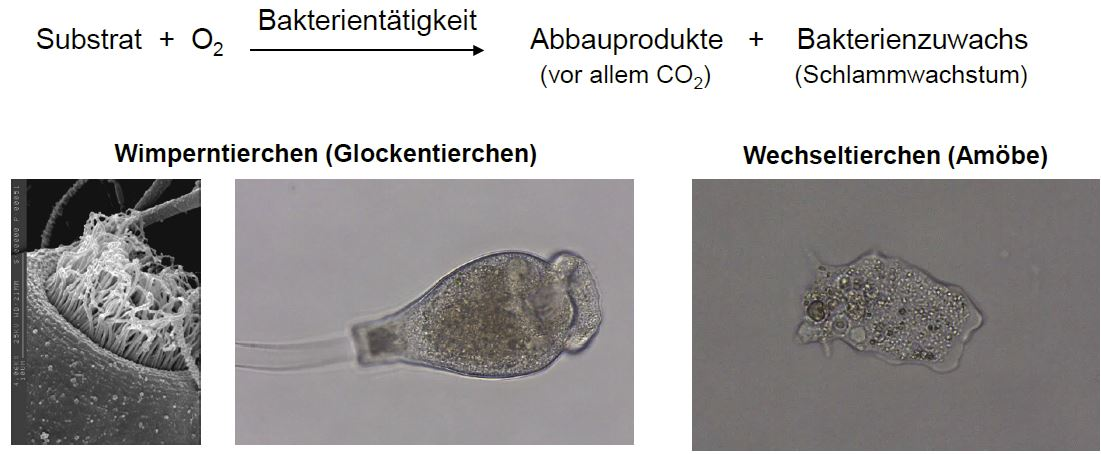
\includegraphics[width=0.8\textwidth]{images/tierchen}
\end{center}
\paragraph{Verfahrensarten}\index{Verfahrensarten} Das verbreitetste Verfahren bei ARAs ist der Durchflussreaktor, auch\index{Verfahrensarten!Belebtschlammverfahren (Durchflussreaktor)} Belebtschlammverfahren genannt. Der Betrieb kann sowohl kontinuierlich\index{kontinuierlich} oder diskontinuierlich\index{diskontinuierlich} (Batch-Betrieb) sein. Es handelt sich dabei um einen sehr robusten Prozess, welches im Notfall künstlich angeimpft werden kann. Der Nachteil sind hohe Investitionskosten, hoher Energiebedarf und die Empfindlichkeit gegen hydraulische Überlastung. Für die Belebung muss das Becken belüftet werden! Weitere Verfahren sind Festbett- (Tropf-, Tauchkörper)\index{Verfahrensarten!Festbettreaktoren} \index{Verfahrensarten!Tropfkörperverfahren}\index{Verfahrensarten!Tacuhkörperverfahren} oder Schwebebettreaktoren\index{Verfahrensarten!Schwebebettreaktoren}. Diese Membranbioreaktoren (MBR) sitzen fest auf einer Membranoberfläche. Sie kommen vor allem bei Kleinstanlagen, Hütten oder abgelegenen Höfen zum Einsatz. 
\paragraph{Belebtschlammverfahren}\index{Belebtschlammverfahren} Die mittlere Aufenthaltszeit\index{Aufenthaltszeit} des Abwassers beträgt bei horizontaler Durchströmung 4-8 Stunden. Der Belebtschlamm hat eine mittlere Aufenthaltszeit von 15 bis 25 Tage (Schlammalter)\index{Schlammalter}. Es handelt sich beim Belebtschlamm um Mineralpartikel mit aufgewachsener Biomasse \index{Biomasse}(ca. 3g/Liter). Diese werden durch die Belüftung in Suspension\index{Suspension} gehalten (in Schwebe). Der Rücklaufschlamm\index{Rücklaufschlamm} durchläuft mehrere Zyklen mittels eines internen Rücklaufs. Diese werden an schwankende Wasserqualität und an das Schlammalter angepasst. Der Überschussschlamm wird in den Faulturm geleitet. Die folgende Abbildung zeigt die Verfahrensführung beim Belebtschlammverfahren. Für die Nitrifikation und Denitrifikation wird ein minimales Schlammalter von 12 Tagen benötigt. Die Gestaltung des Beckens hängt vom gewünschten Schlammalter ab. Weiter soll eine minimale Sohlenströmung erzielt werden. In der Regel sind die Becken vier bis fünf Meter tief. 
\begin{center}
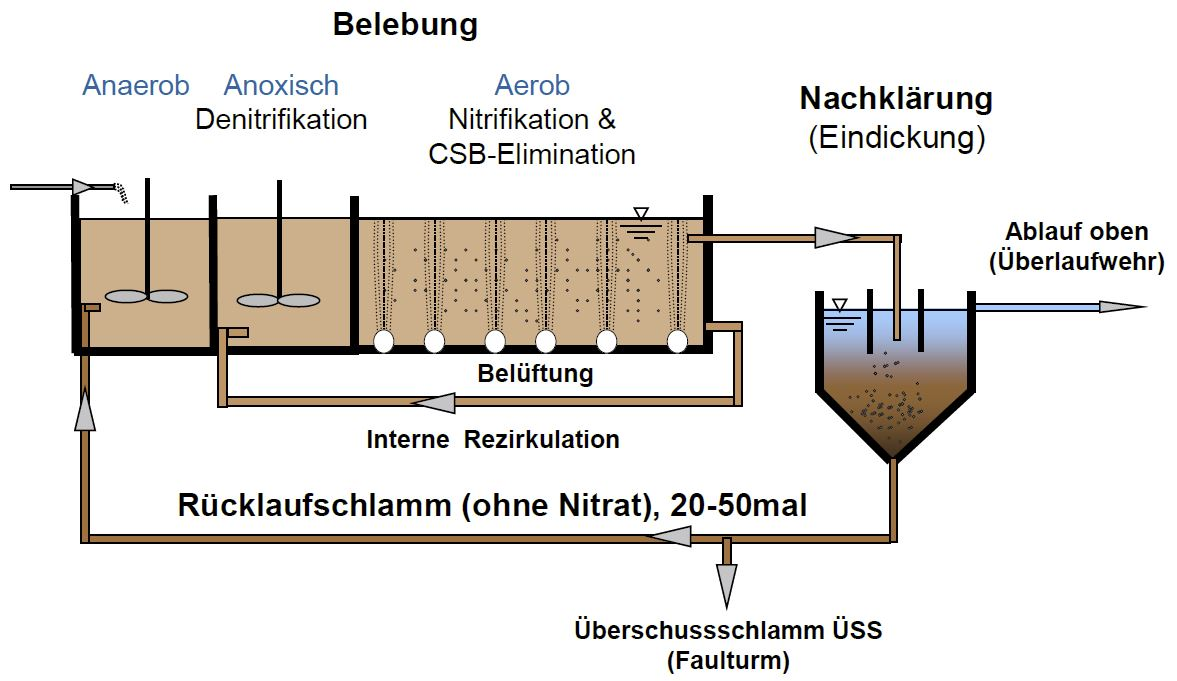
\includegraphics[width=0.7\textwidth]{images/belebt}
\end{center}
\paragraph{Verfügbarkeit von Sauerstoff} Die Verfügbarkeit von Sauerstoff\index{Verfügbarkeit von Sauerstoff} lässt sich auf chemische und biologische Bedingungen beziehen. Auf biologische Bedingungen bezogen:\index{Anaerob} Anaerob: kein bioverfügbarer Sauerstoff vorhanden /\index{Aerob} Aerob: im Wasser gelöster Sauerstoff vorhanden (Sauerstoff bioverfügbar). Auf chemische Bedingungen bezogen:\index{Anoxisch} Anoxisch: kein gelöster Sauerstoff vorhanden, aber dafür andere Sauerstoffträger\index{Sauerstoffträger} wie $SO_4$, $PO_4$, $NO_2$, $NO_3$, etc.\[\begin{split} \textrm{Atmung (aerob):} & C_6H_{12}O_6 + 6O_2 \rightarrow 6 CO_2 + 6 H_2O\\ &\textrm{Zucker + Sauerstoff} \rightarrow \textrm{Kohlenstoffdioxid + Wasser}\\ \textrm{Gärung (anaerob):}   & C_6H_{12}O_6 \rightarrow 2CO_2 + 2 C_2H_5OH\\ &\textrm{Zucker} \rightarrow \textrm{Kohlenstoffdioxid + Ethanol}\\ \textrm{Denitrifikation (anoxisch):} & 6NO_3^- + 5CH_3OH \rightarrow 5CO_2 + 7H_2O + 6OH^- + 3N_2\\ 
& \textrm{Nitrat + Methanol} \rightarrow \textrm{Kohlenstoffdioxid + Wasser + Hydroxidionen + Stickstoff}
\end{split}\]
\paragraph{Nitrifikation und Denitrifikation}\index{Nitrifikation}\index{Denitrifikation}
\begin{center}
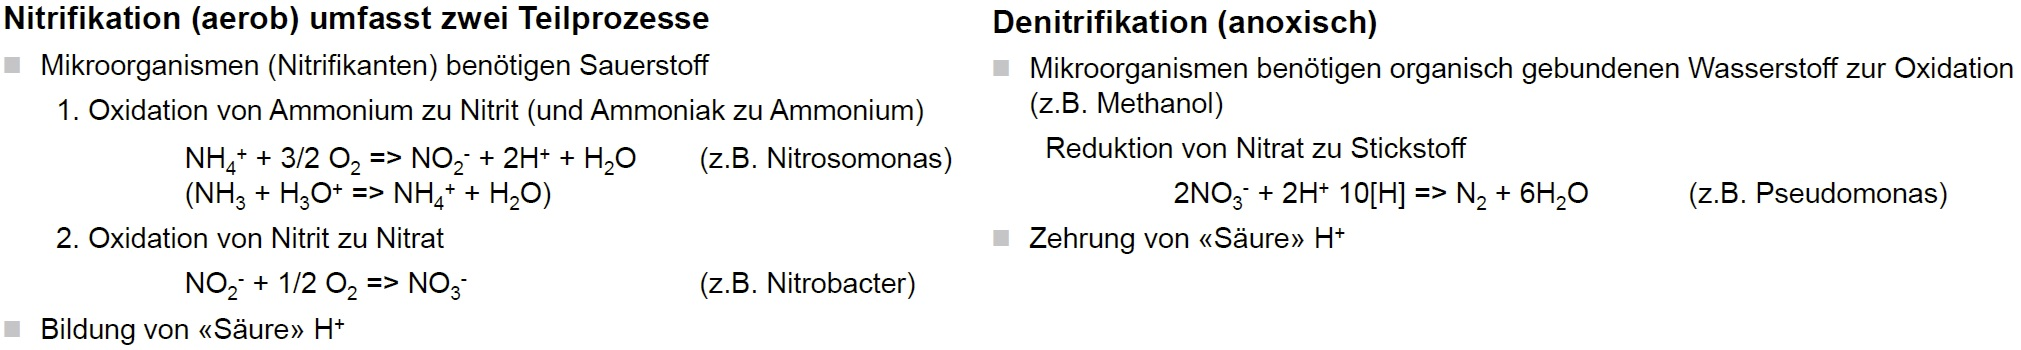
\includegraphics[width=1.1\textwidth]{images/nitrifikationdenitrifikation}
\end{center}
Für diese Prozesse wird Sauerstoff benötigt. Für die Umsetzung\index{Umsetzung TKN} von 1kg TKN in N\textsubscript{2} wird 1.5 g Sauerstoff benötigt. Für die Umsetzung\index{Umsetzung BSB\textsubscript{5}} von einem Kilogramm BSB\textsubscript{5} wird zirka 35m\textsuperscript{3} Luft benötigt, was rund 60\% der Betriebskosten ausmacht (ca. 2mg/L O\textsubscript{2}). Es gibt verschiedene Anordnungen für die Denitrifikation in einer ARA. Die Nachgeschaltete Denitrifikation ist in der Schweiz wenig verbreitet. Die Vorgeschaltete Denitrifikation ist am weitesten verbreitet in der Schweiz. Daneben gibt es die Simultane Denitrifikation (intermittierend), welche in der Schweiz momentan nur in der ARA Werdhölzli anzutreffen ist.
\begin{center}
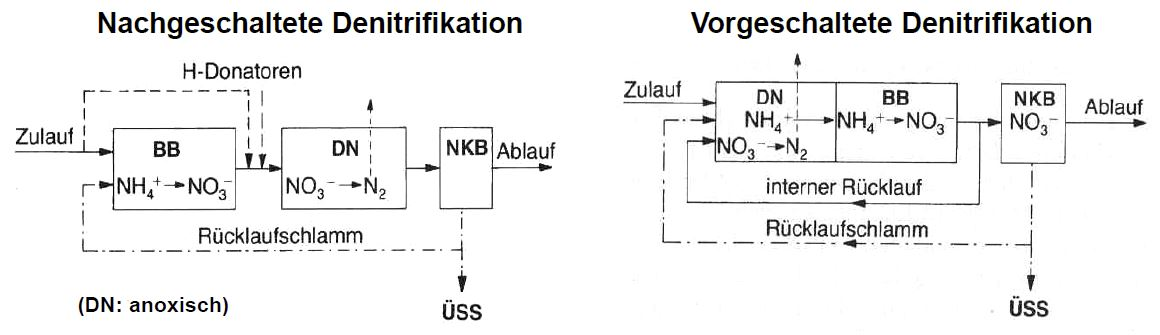
\includegraphics[width=0.7\textwidth]{images/anordnungnitri}
\end{center}
\paragraph{Nachklärung} Die Nachklärung\index{Nachklärung} dient der Bildung einer gut absetzbaren Flockenstruktur und der kontinuierliche Abscheidung von Belebtschlamm. Der Überschussschlamm wird in den Faulturm geleitet. Der Trockenrückstandanteil (TR) des Klärschlamms beträgt rund 6\%. Bei der Faulung wird rund die Hälfte der organischen Stoffe abgebaut. Im Klärschlamm darf der Schwermetallgehalt nicht zu hoch sein. 
\subsection{3. Stufe: Chemische P-Fällung}\index{Chemische P-Fällung}\index{Chemische Reinigungsstufe} \index{3. Stufe}
Gemäss der Gewässerschutzverordnung müssen ARAs im Einzugsgebiet von Seeen und ARAs $\geq$ 10'000 EW unterhalb von Seen den Wert von 0.8 mg P\textsubscript{tot} pro Liter einhalten (24 h -Sammelprobe). Kantonal gelten zum Teil verschärfte\index{P-Elimination! Werte} Anforderungen. Zum Beispiel am Zürichsee: 0.2 mg P\textsubscript{tot} pro Liter und am Bodensee: 0.3 mg P\textsubscript{tot} pro Liter. In der Schweiz sind 610 der 760 Kläranlagen mit einer P-Elimination ausgerüstet.
\paragraph{P-Elimination} Partikulärer Phosphor\index{Partikulärer Phosphor} wird mit anderen Feststoffen über Sedimentation abgeschieden (z.B. in der mechanischer Reinigung). Bei gelöstem Orthophosphat\index{Orthophosphat} muss das Anion durch Fällung entfernt werden. Die P-Verbindungen werden dann mit gut absetzbaren Partikeln über den Schlamm aus dem Abwasser entfernt. Das Verfahren zur chemischen P-Elimination sieht wie folgt aus:\index{P-Elimination! Verfahren}
\[Me^{3+} + PO_4^{3-} \Rightarrow Me(PO)_4\downarrow + Me (OH)\]
Die Wirksamkeit der Fällung ist abhängig von der Einmischung (Vor-, Simultan-, Nach-, Kombinationsfällung), dem Beta-Wert, dem pH-Wert, dem $Ca^{2+}$ Anteil und der Effizienz der Partikelabscheidung (Sedimentation / Filtration).
\paragraph{Fällungsprodukte} Durch die Zugabe von $Al^{3+}$ oder $Fe^{3+}$ entstehen Fällungsprodukte wie $Fe(PO_4)x(OH)_3-3x(H_2O)y$. Der pH-Wert ist dabei entscheidend für die Bildung von P-Komplexen. Die Dosiermenge ist auch durch Ablaufgrenzwert bestimmt.\index{P-Elimination! Fällungsprodukte}
\paragraph{P-Fällung} Die Entfernung von Orthophosphat und P-haltiger Partikel geschieht durch drei Prozesse: Fällung, Adsorption und Flockung. Die Abtrennung von P-haltigen Feststoffen erfolgt durch Sedimentation und Filtration. Bei\begin{wrapfigure}[12]{r}{8cm} 
  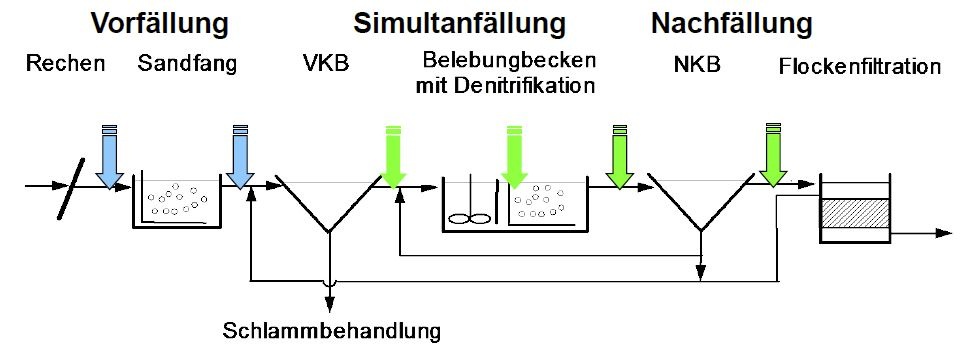
\includegraphics[width=.5\textwidth]{images/faellung}
\end{wrapfigure} der Fällung werden Hydroxo-Phosphat-Komplexe gebildet. Bei der Adsorption findet eine Selektive Anlagerung von Phosphaten an Fe-Hydroxid-Niederschlägen statt. Bei der Flockung werden Entstabilisierte P-haltige Kolloide durch \index{P-Elimination! Fällmittel}
Adsorption polynukleare Hydroxokomplexe und Agglomeratbildung zu grösseren Flocken.\\ \\
Mehrere Fällmittel sind verfügbar und erprobt. Die verbreitetsten Mittel in Lösung sind: Eisenchloridsulfat (FeCISO\textsubscript{4}) und Eisenchlorid (FeCl\textsubscript{3}). Die Wahl erfolgt aufgrund der Kosten, der Verfügbarkeit, der Lieferantenbeziehungen etc.\begin{wrapfigure}[12]{r}{7cm} 
  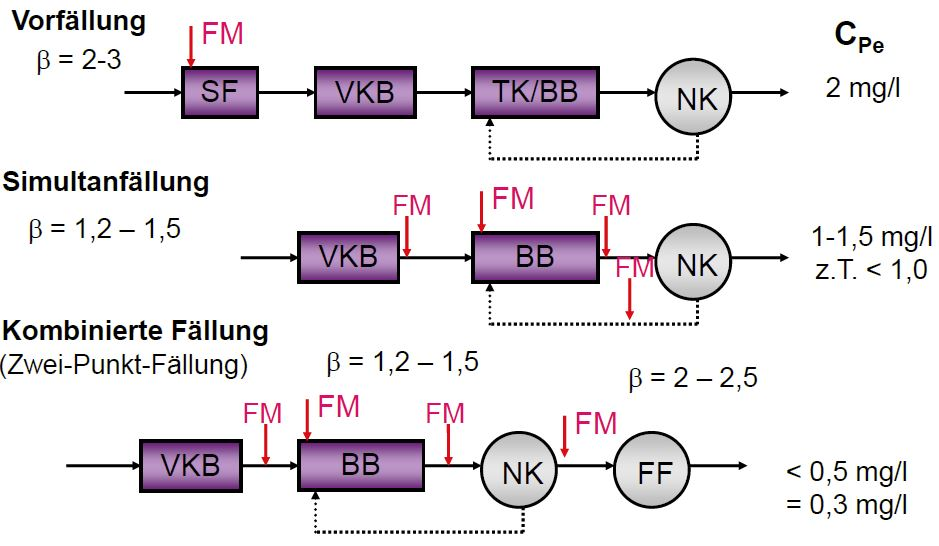
\includegraphics[width=.45\textwidth]{images/dosierung}
\end{wrapfigure}
\paragraph{Verfahren der Einmischung}\index{P-Elimination! Einmischung} Die Effizienz kann deutlich gesteigert werden durch optimale Dosierung und Verteilung des Fällmittels. Damit verbessert sich auch die Abscheidung von Fällprodukten und zusätzlicher Biomasse mittels Sandfiltration. Eine Zwei-Punkt-Fällung (Kombination aus Simultan-und Nachfällung) erhöht die Eliminationsleistung bei gleichem Fällmitteleinsatz. So werden sehr tiefe P\textsubscript{tot} - Ablaufwerte erreicht. Die Investitionskosten sind jedoch dem entsprechend hoch. 
\paragraph{Bemessung der Dosierung}\index{P-Elimination! Dosierung} Der \index{Beta-Wert} Beta-Wert beschreibt die relative Fällmittelmenge [mol Me/mol X\textsubscript{P,Fäll}]. Die Einleitung des Fällmittels\index{Fällmittel} muss an einer Stelle geschehen, wo eine möglichst gute Durchmischung gewährleistet ist. Daher sollte eine Einleitung nicht am Rand eines Beckens erfolgen. Besser ist die Zuleitung an einem Rinnenknick oder noch besser ist es, wenn die Dosierung durch Injizierung von mehreren Seiten auf dem gesamten Durchflussquerschnitt erfolgt. Die Zugabe beim Hebewerk ermöglicht zwar eine gute Durchmischung, dafür besteht jedoch die Gefahr der Korrosion, da die Fällmittel sehr aggressive sind. Die Fällung hat einen Einfluss auf verschiedenste Prozesse in der ARA. Da Phosphor ein zentraler Nährstoff in der Landwirtschaft ist und eine endliche Ressource darstellt, wird ein Recycling von Phosphor aus dem Schlamm angestrebt. 
\paragraph{Betriebliche Aspekte} Durch die Fällung erhöht sich der spezifische Schlammanfall\index{Schlammanfall}. Die Absetzeigenschaften des belebten Schlamms wird verbessert durch einen besseren Schlammindex und weniger Schlammabtrieb. Der Schwermetallgehalt im Schlamm ist absolut gesehen höher. Der Nährstoffgehalt im Schlamm ist höher, jedoch schlecht pflanzenverfügbar. Der Brennwert wird durch den höheren Anteil an anorganischen Stoffen verringert. Die Chlorid- und Sulfatkonzentrationen im Ablaufwasser steigen (Aufsalzung)\index{Aufsalzung}. Die Fällung hat keinen Einfluss auf die biologischen Prozesse bei der Nitrifikation.
\subsection{4. Stufe: Mikroverunreinigungen}\index{Mikroverunreinigungen}\index{4. Stufe}
Heute werden in den Fliessgewässern zum Teil bereits Organische Pestizide über dem Grenzwert von $0.1\mu g/ Liter$ je Einzelstoff nachgewiesen. Chronische Qualitätskriterien (CQK) werden von einzelnen Biozidprodukten und Pflanzenschutzmitteln überschritten. Die Mikroverunreinigungen werden in den meisten Kläranlagen nicht zurückgehalten. Zudem weisen viele Wirkstoffe, zum Beispiel in Pharmaka, sehr geringe Abbauraten auf. Die Mikroverunreinigungen sollen zu 50\% reduziert werden, in dem 100 Kläranlagen zu über 80\% Spurenstoffe (Leitsubstanzen) entfernen. Die Investitionskosten betragen rund 1.2 Milliarden Franken zudem steigen die Betriebskosten und der Energiebedarf um 10 bis 20\%. 
\paragraph{Ziele und Erfolgskontrolle} Das Ziel ist es die aquatischen Ökosysteme zu schützen. Weiter sollen die Wasserressourcen geschützt werden. Dies soll durch eine Verantwortung flussauf- und flussabwärts erreicht werden. Ziel ist ein Reinigungseffekt von 80\% für organische Spurenstoffe. Heute liegt dieser Effekt bei 20-40\%, sodass eine Verdoppelung des Reinigungseffektes für gut ausgebaute ARA vorgesehen ist. Die Überprüfung des Reinigungseffekts erfolgt anhand von 12 Leitsubstanzen. Die Kantone wählen aus diesen 12 Substanzen 5 aus zur Überprüfung des Reinigungseffekts. Der\index{Reinigungseffekt} Reinigungseffekt ist als Mittelwert der 5 Substanzen definiert, wobei jedoch jede Probe eingehalten sein muss. Die Stoffliste wird periodisch, alle fünf Jahre, angepasst. Der Probenahmezeitraum beträgt 48 Stunden und die Probenahmehäufigkeit wird abgestuft nach der ARA-Grösse vorgegeben. Beispiel ARA Neugut (EW = 105'000): täglich 20-50 Mio. Liter Abwasser, Elimination der organischen Schmutzstoffe zwischen 96 und 99\% und der Mikroverunreinigungen zwischen 80 und 90\%. Es ist die erste volltechnische Ozonanlage (Stand 2014).
\section{Versickerung} \index{Versickerung}
\paragraph{Lockergesteine}\index{Lockergestein} Gemäss der Terminologie der SN 6700009 sind Lockergesteine ein Gemisch von Steinen, die durch Aufschütteln im Wasser nach Korngrössen zerlegt werden können. Sie entstehen durch Verwitterung, Abtrag (Erosion, Rutschung) oder Transport und Ablagerung (Sedimentation). Es ist das Ausgangsmaterial der Bodenbildung. Bei Wassersättigung bildet es den Porengrundwasserleiter. \index{Porengrundwasserleiter}
\begin{center}
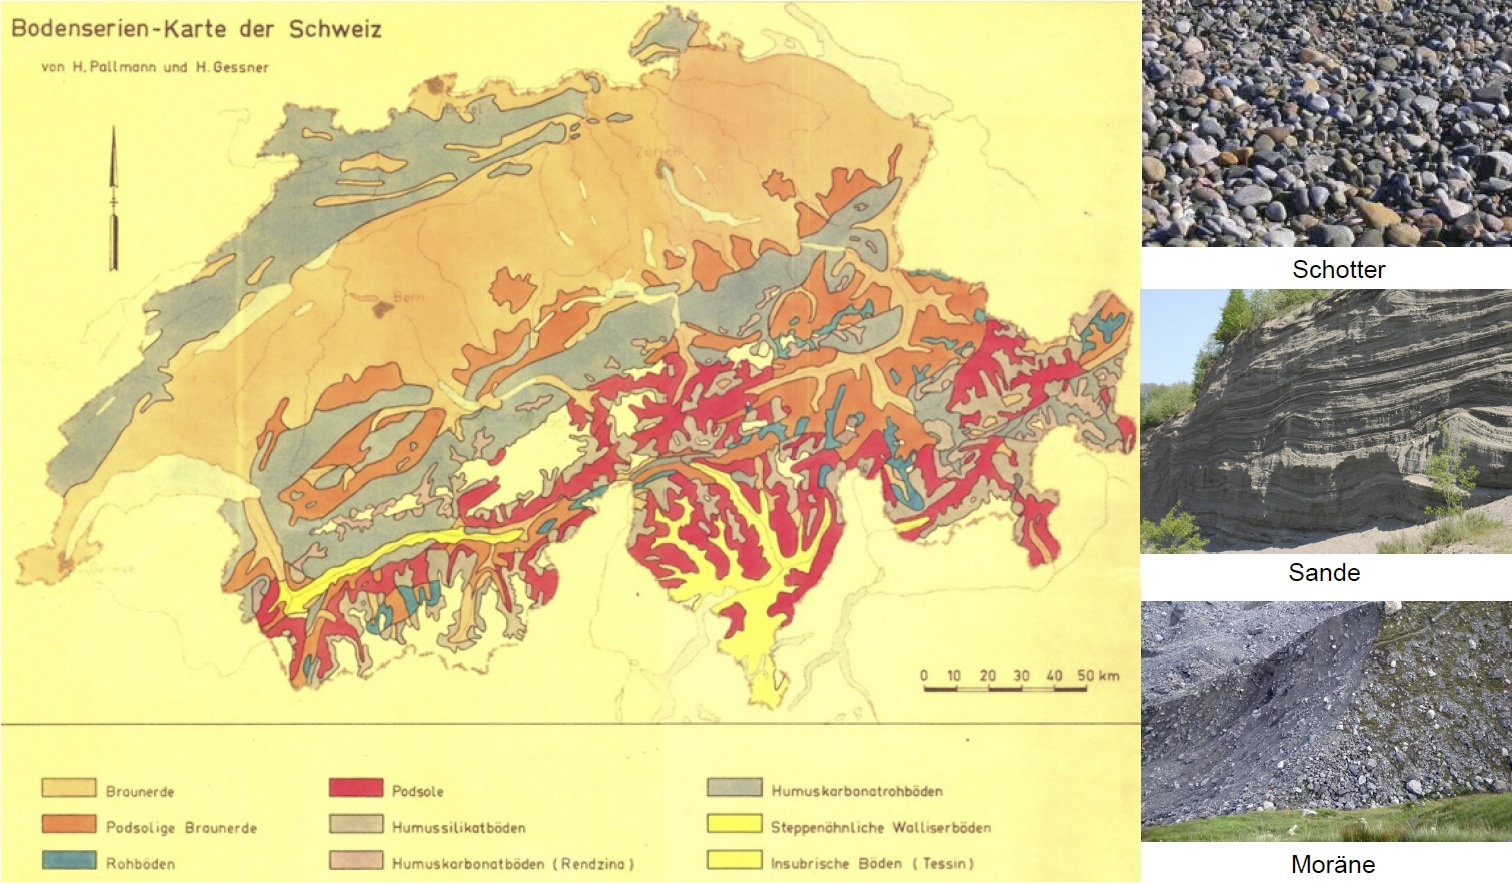
\includegraphics[width=0.65\textwidth]{images/geologisch}
\end{center}
Die Kleinräumliche Anordnung der Böden sind Folge der geomorphologischen Prozesse (Wasserregime etc.). 
\paragraph{Boden- und Grundwasser} Als Bodenwasser\index{Bodenwasser} bezeichnet man das Wasser in der ungesättigten Zone, welches vom Boden gegen die Schwerkraft gehalten wird. Im\index{Kapillarwasserraum} Kapillarwasserraum kann das Wasser entgegen der\begin{wrapfigure}[14]{r}{7cm} 
  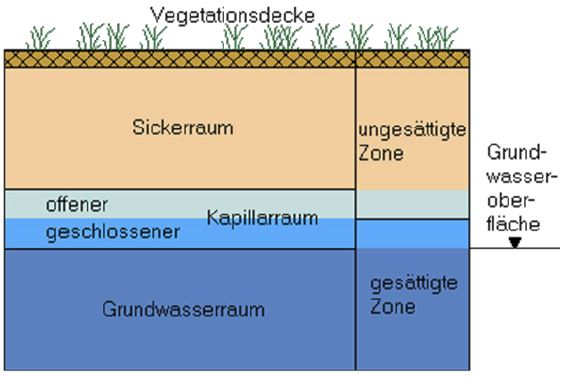
\includegraphics[width=.45\textwidth]{images/bodenraum}
\end{wrapfigure} Schwerkraft aufsteigen. Als Stauwasser\index{Stauwasser} wird Wasser bezeichnet, das nur einen Teil des Jahres vorhanden und auf einer Wasserundurchlässigen Schicht aufliegt. Das Kristallwasser\index{Kristallwasser} ist auch nach der Trocknung bei 105 Grad noch gebunden. Als Grundwasser\index{Grundwasser} bezeichnet man das Wasser in der gesättigten Zone. Es füllt alle Hohlräume zusammenhängend aus und kann sich durch die Schwerkraft bewegen. Je Feinkörniger ein Boden, desto schlechter fliesst das Wasser ab.
\paragraph{Aggregierung (Gefüge)}\index{Aggregierung} Die Korngrössenverteilung gilt per Definition nur am mineralischen Teil des Bodens. Alles über 2mm Korndurchmesser ist Kies, kleiner als 0.063 ist Silt\index{Silt} und kleiner als 0.02mm ist Ton. Sekundärporen\index{Sekundärporen} (Grobporen)\index{Grobporen} im Boden sind anfällig für Verdichtung. Die Korngrössenverteilung gibt Hinweise auf mögliche Aggregatstrukturen. Weiter wird zwischen verschiedenen Gefügeformen unterschieden:
\begin{itemize}
\item Elementar- oder Einzelkorngefüge: Mineral- und Humuspartikel liegen isoliert nebeneinander, z.B. loser Sand
\item Kohärent- oder Hüllengefüge: Mineral- und Humuspartikel bilden dichte Packung, z.B. grössere Mineralkörner mit Umhüllungen von Huminstoffen und Ton
\item Aggregat- oder Aufbaugefüge: Mineral- und Humuspartikel bilden Aggregate unterschiedlicher Grösse und Form, z.B. Krümel (1-10 mm), Bröckel (10 mm)
\item Segregations- oder Absonderungsgefüge: Tonfraktion bilden Absonderungsformen durch Austrocknung / Schrumpfung als Polyeder, Prismen, Säulen oder Platten
\end{itemize}
Die Aggregierung hat einen grossen Einfluss auf die Versickerung (Wasserdurchlässigkeit), Durchlüftung und Bodenfruchtbarkeit. Ein lockeres Gefüge wird angestrebt.
\paragraph{Kapillare Steighöhe (Kapillarraum)}\index{Kapillare Steighöhe} Die Kapillare Steighöhe und die Durchlässigkeit\index{Durchlässigkeit} hängen zusammen. Je geringer die Durchlässigkeit, desto höher steigt das Wasser. Als Faustregel gilt: \[h_k[cm] \approx\dfrac{1}{\sqrt{k}}\] k ist dabei die Durchlässigkeit. Für einen Ton mit d\textsubscript{10} = 0.002mm und d ungefähr 0.0002 mm folgt eine kapillare Steighöhe von zirka 1.5 Meter. Bei Sanden können grössere Zugkräfte auftreten, als es sich aus der kapillaren Steighöhe ergeben würden. Durch Anstieg des Grundwasserspiegels werden diese Zugkräfte aber unwirksam. Allgemein ist beim Aufstieg die weiteste Kapillare massgebend (aktive kapillare Steighöhe) und beim Abstieg die engste Kapillare (kapillares Rückhaltevermögen).
\subsection{Integrale Regenwasserbewirtschaftung}
Das Ziel ist es, wenn möglich, möglichst viel Niederschlagswasser vor Ort zu versickern. Hinweise zur Regenwasserversickerung\index{Regenwasserversickerung} finden sich in der Norm SN 592'000 und den VSA Richtlinien Regenwasserentsorgung und Abwasserbewirtschaftung bei Regenwetter. 
\begin{center}
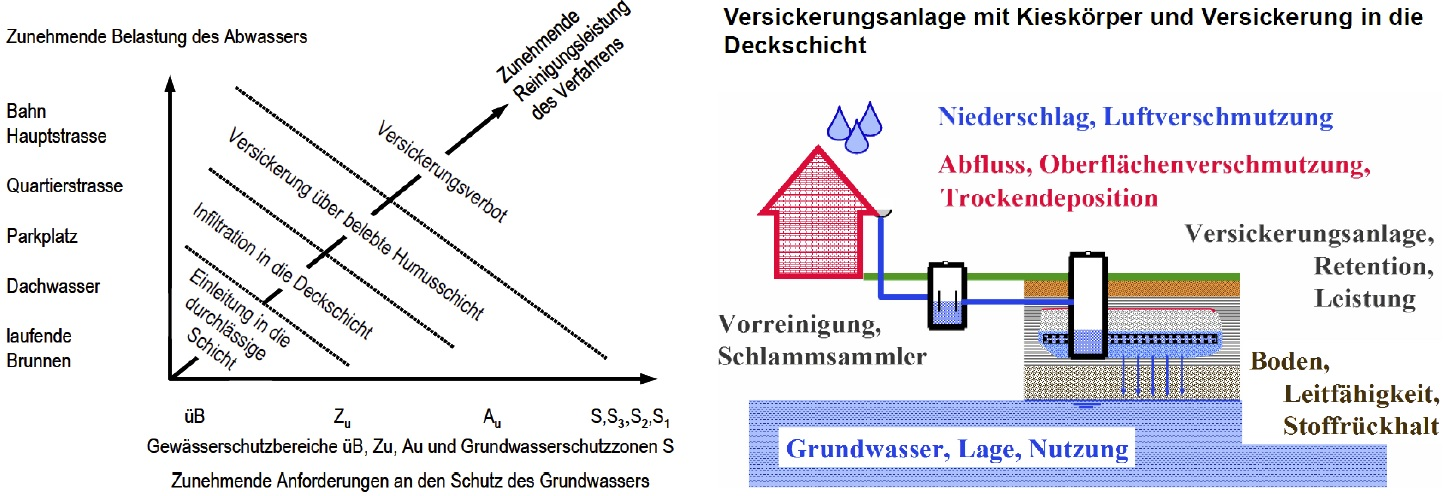
\includegraphics[width=.8\textwidth]{images/versickerungbelastung}
\end{center}
Bevor jedoch eine Versickerungsanlage\index{Versickerungsanlage} gebaut werden kann, muss geprüft werden, ob eine Versickerung von verschmutztem Regenabwasser erlaubt ist. Die Anforderungen an die Versickerungsanlage sind abhängig von der Belastung des Abwassers und dem gewünschten Schutz des Grundwassers. Die VSA-Richtlinie gibt Hinweise zu den Belastungen des Regenwassers. Bei Verschmutzung gilt ein Behandlungsgebot oder Versickerungsverbot. Weiter finden sich im GEP oder im Versickerungskataster Hinweise darauf, ob eine Versickerung möglich ist.
\paragraph{Einzugsgebiet: Reduzierte Fläche} Die Reduzierte Fläche F\textsubscript{red} ist eine fiktive Hilfsgrösse, um unterschiedlich strukturierte Teileinzugsgebiete zu einer gemeinsamen, abflusswirksamen Grösse zusammenzufassen. Die reduzierte Fläche wird mit der Einheit ha\textsubscript{red} angegeben und entspricht ungefähr dem undurchlässigen, versiegelten Anteil des Einzugsgebiets. Mit $Q_R$ lassen sich die Abflussmengen schätzen. Für Einzelflächen gilt: $Q_R = r \cdot \psi \cdot F$ mit $Q_R$ = Regenabfluss an einer bestimmten Stelle im Kanalnetz in Liter pro Sekunde, $r$ = Regenintensität in Liter pro Sekunde und Hektare, $\psi$ = Abflussbeiwert\index{Abflussbeiwert} und der Fläche des Einzugsgebiets $F$ in Hektaren. Die Reduzierte Fläche entspricht der Fläche des Einzugsgebiets multipliziert mit dem Abflussbeiwert. Daraus folgt für viele Teileinzugsgebiete die Formel:\[Q_R = r \cdot \sum F_{red,i} = r \cdot \sum F_i \cdot \psi_i\]\index{reduziertes Einzugsgebiet}
\paragraph{Retention: Volumen}\index{Retentionsvolumen}
\begin{center}
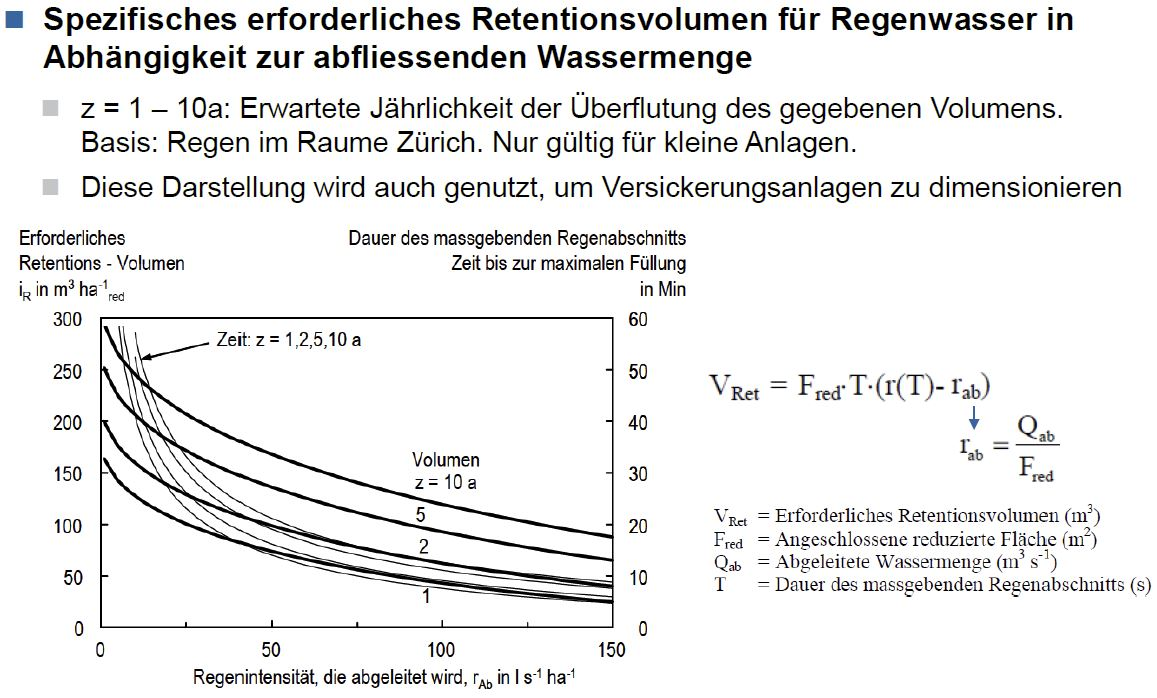
\includegraphics[width=.8\textwidth]{images/retentionsvolumen}
\end{center}
\paragraph{Korngrössenverteilung}\index{Korngrössenverteilung} Im Labor wird die Korngrössenverteilung mittels einer Nass- oder Trockensiebung erstellt. Dies gilt für die Kornfraktionen grösser als 0.063mm. Die Siebe sind genormt und werden zu Siebtürmen\index{Siebanalyse} zusammengesetzt. Die kleineren Fraktionen werden über Sedimentationsverfahren\index{Aräometer} (Aräometer-Verfahren, Laserbeugung LBS)\index{LBS} \index{Laserbeugung} bestimmt. Aus den resultierenden Sieblinien können die Kennwerte abgelesen werden. Zum Beispiel der Mittlere Korndurchmesser (d\textsubscript{50}). Weiter lässt sich der Ungleichförmigkeitsgrad Cu bestimmen. Wenn Cu = 1 wird, ist es eine gleichförmige Verteilung. Der Feinanteil bestimmt die kalkulierbare Sickerleistung. Bei viel Feinanteil kann es zur Kolmation kommen, bei der die Feinteile umgelagert werden und den Boden so \glqq dicht machen.\grqq Das Gefüge ist von der Bodenart und der Bodenbildung (Zeit) abhängig. \index{Cu} \index{Cc}
\begin{center}
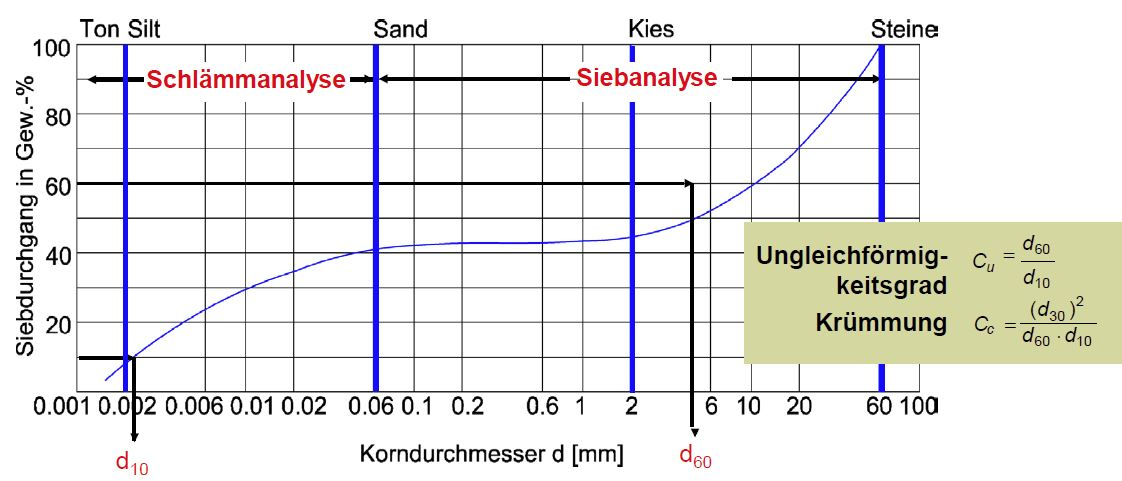
\includegraphics[width=\textwidth]{images/siebkurve}
\end{center}
\paragraph{Sickerfähigkeit} Die Druchlässigkeitsbeiwert\index{Druchlässigkeitsbeiwert} wird im Labor mit einem Lysimeter bestimmt. Der Druchlässigkeitsbeiwert (Permeabilität)\index{Permeabilität} bezeichnet den Widerstand des Bodens bei laminarer, stationärer Wasserströmung\index{k} k (cm/s)(Gesetz nach Darcy)\index{Darcy}. Einen Einfluss hat die Strukturform und der Feinanteil. Vor allem das Skelett ist massgeblich und die Feinanteile limitieren die Durchlässigkeit. Weiter spielt die Lagerungsdichte\index{Lagerungsdichte} beziehungsweise die Porenzahl eine Rolle.\[v = k \cdot i \textrm{ oder } v = Q/F \textrm{ oder } k = v/i \textrm{ oder } k = Q \cdot l / F \cdot H\]
Dabei ist v die Filtergeschwindigkeit\index{Filtergeschwindigkeit}, Q die Durchflussmenge, F der gesamte durchströmte Querschnitt und i = H/l ist das hydraulische Gefälle, welches der Potentialdifferenz H geteilt durch die Länge des Sickerweges l ist. Dabei ist k die gesättigte Wasserdurchlässigkeit, welche auch nach HAZEN abgeschätzt werden kann. Für gleichförmige Sande ist $k \approx 100 \cdot d_{10}^2$ Für ungleichförmige Materialien ist $k = 100 \cdot d_{10}^2 / Cu $ mit $Cu = d_{60}/d_{10}$.
\paragraph{Spezifische Sickerleistung}\index{spezifische Sickerleistung} Die spezifische Sickerleistung beschreibt die Versickerung im ungesättigten Boden. Sie wird mittels Versickerungsversuchen oder aus der gesättigten Wasserleitfähigkeit hergeleitet. $s_{spez} = k/2$ Diese\begin{wrapfigure}[14]{r}{8.5cm} 
  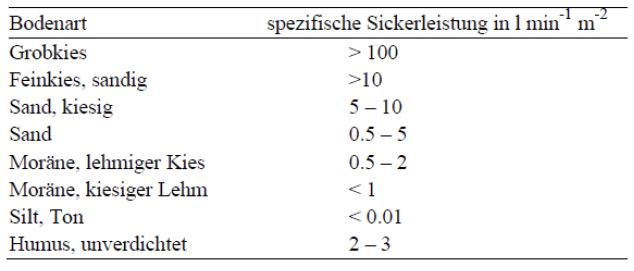
\includegraphics[width=.55\textwidth]{images/spezsicker}
\end{wrapfigure} Formel basiert auf den Annahmen, dass der hydraulische Gradient = 1 ist und der Abstand zwischen der Versickerungssohle und dem Grundwasserspiegel zwischen einem und sechs Meter liegt. Damit kann die Formel für Versickerungsanlagen mit 2 bis 4 m Tiefe als grobe Näherung zur Ermittlung der spezifischen Sickerleistung verwendet werden. Bei Versickerungsversuchen wird im Feld ein Loch ausghoben und anschliessend die Versickerung durch die Bestimmung des Wasserstands berechnet. Am genausten sind die Ergebnisse bei der Verwendung eines Doppelringinfiltrometers.\index{Infiltrometer}  Dabei sollte der äussere Ring stationäre Verhältnisse aufweisen, bevor im inneren Ring gemessen wird.\clearpage
\paragraph{VSA Anforderungen an den Boden} Die neue VSA Richtlinie ab 2019 enthält andere Anforderungen als die Richtlinie von 2008. 
\begin{center}
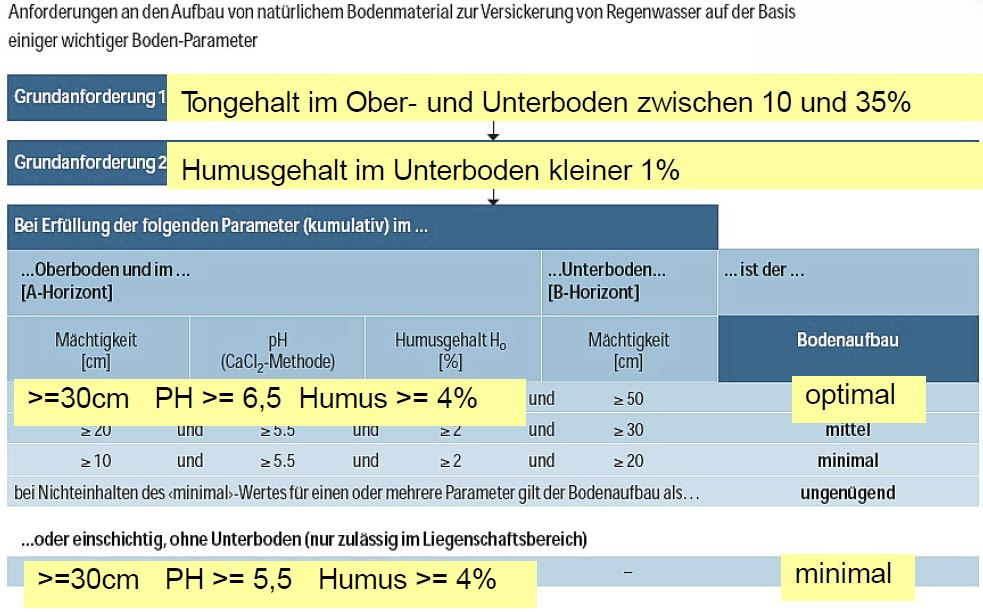
\includegraphics[width=0.8\textwidth]{images/vsaboden}
\end{center}
\paragraph{Einleitung in ein Gewässer} Vor der Einleitung in ein Oberflächengewässer muss geprüft werden ob diese auch zulässig ist. Weiter ist eine Einleitung mit dem Gewässerschutzamt des Kantons abzusprechen. In der Regel sind 10 bis 50 Liter pro Sekunde problemlos Einleitbar und werden meist bewilligt. Die Einleitung erfolgt über einen Schlammsammler und anschliessend führt ein Rohr zur Vorflut. Meist wird noch eine Retention vorgeschaltet.
\paragraph{Sickersysteme} Die folgende Abbildung bietet eine Grobentscheidung für das Versickerungssystem auf der Basis der Dimensionierung. Die unteren Detailabbildungen stellen verschiedene Varianten dar.
\begin{center}
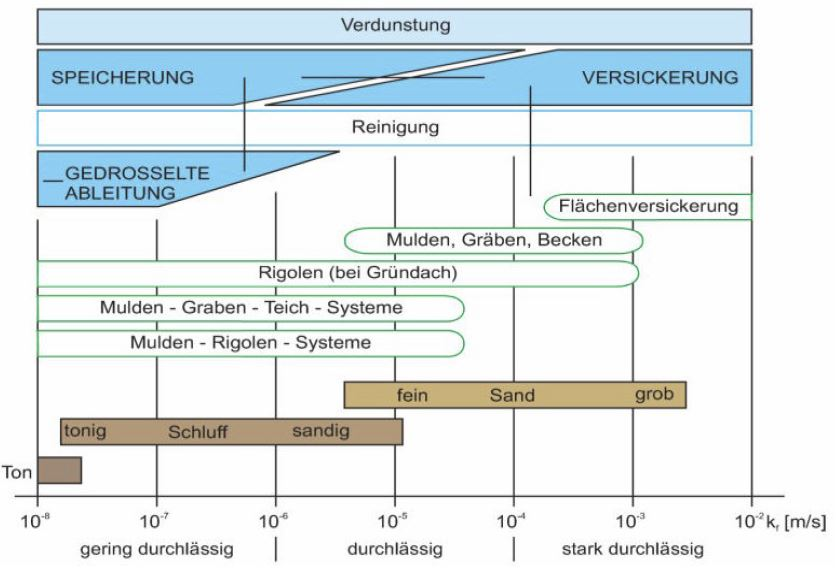
\includegraphics[width=0.8\textwidth]{images/sys}
\end{center}
\begin{center}
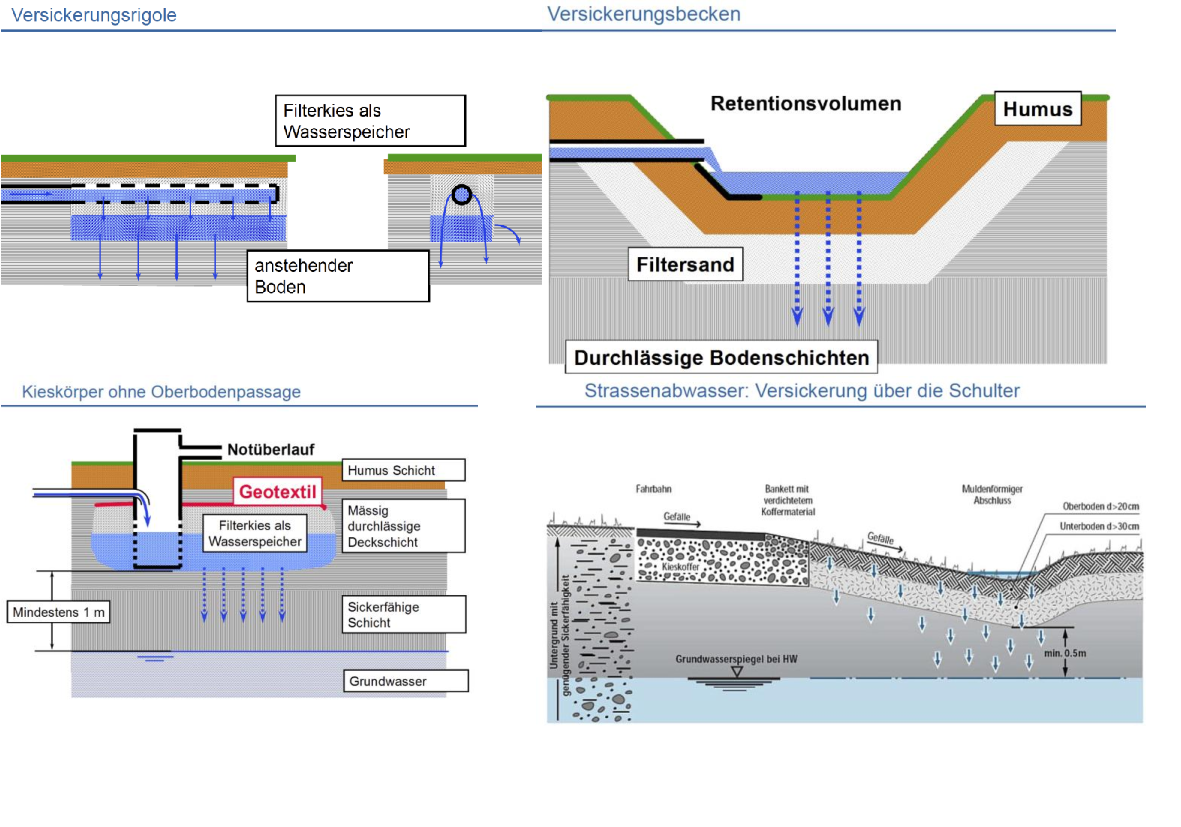
\includegraphics[width=\textwidth]{images/versick}
\end{center}\index{Versickerungssysteme}
\paragraph{Berechnung des Retentionsvolumens}\index{Retentionsvolumen Berechnung} Die Sickerleistung\index{Sickerleistung} des bewachsenen Oberbodens beträgt zwischen einem und drei Liter pro Minute und Quadratmeter. Begrenzend für die Sickerleistung ist die gesättigte Durchlässigkeit des Unterbodens/ Untergrunds. 
\paragraph{Was ist bei der Planung zu beachten?}Die Anlaufzeit und die Fliesszeit werden vernachlässigt.Daher Gültig eher nur für Einzelliegenschaften. Auf Einzugsgebietsebene können sich durch die unterschiedlichen Anlauf- und Fliesszeiten Abflussspitzen ergeben. Die hier verwendete Methode ist eher ungeeignet für die Abschätzung solcher Situationen. Die Dimensionierungsdiagramme der VSA-Richtlinie gelten bis zu einer Regendauer $<$ 60 Min. Die vorgestellte Berechnung ist für geringe Versickerungsleistungen ($Q_{ab} < 5 l/(s\cdot ha$) nicht geeignet. Die Unterstützung durch eine Modellrechnung ist hilfreich (Niederschlags-Abflussmodell).\clearpage
\paragraph{Beispiele}
\begin{center}
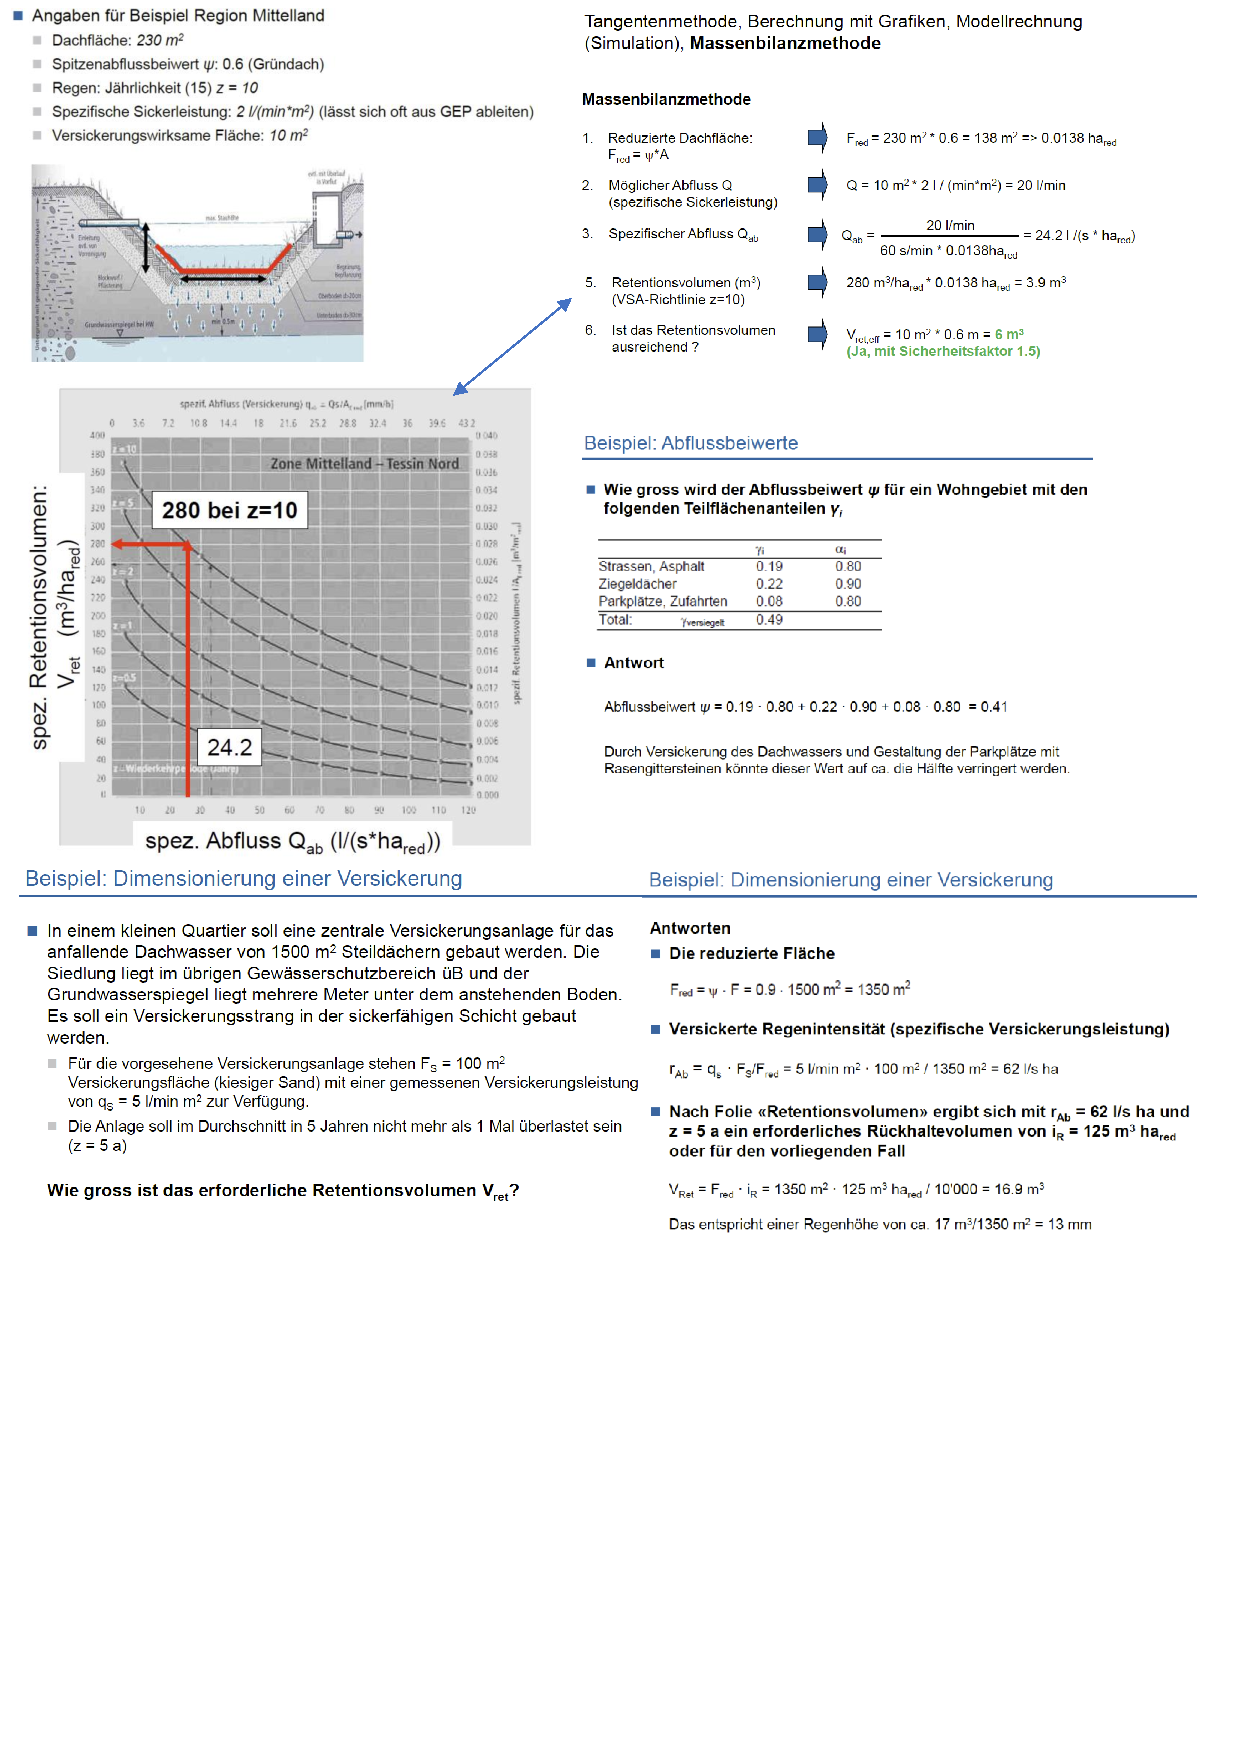
\includegraphics[width=\textwidth]{images/bspversickerung}
\end{center}\index{Versickerung Beispiele} \index{Anflussbeiwerte Beispiel} \index{Dimensionierung Versickerung}
\section{Industrieabwasser} Damit Industrieabwasser\index{Industrieabwasser} in die Kanalisation eingeleitet werden darf, muss es die Einleitbedingungen gemäss Gewässerschutzverordnung Anhang 3.2 erfüllen. Dazu gehört, dass der \index{pH-Wert}pH-Wert zwischen 6.5 und 9 liegt und die Kohlenwasserstoffe KW weniger als 20 mg pro Liter sind. Weiter gibt es Grenzwerte für Schwermetalle und spezifische Anforderungen je Branche. Die Kanalisation ist keine Abfallentsorgungsanlage. Daher kommen in der Industrie häufig mechanische und chemische Verfahren zur Vorklärung zum Einsatz. Zum Teil kopieren sie Prinzipien der Siedlungsentwässerung. Auch gibt es Industrien, die eine Abflusslose Produktion, eine \glqq Cleaner Production\grqq anstreben.
\paragraph{Mineralölabscheider} Im Abscheideraum\index{Abscheideraum} wird das Abwasser beruhigt und die leichteren Teile schwimmen auf. Eine Schwimmerkugel beim Auslauf verhinder das Öl austritt. Das Öl muss regelmässig von einer Unterhaltsfirma abgepumpt werden. Die meisten Mineralölabscheider\index{Mineralölabscheider} werden als Fertigbetonteile eingebaut. Einsatzorte sind Tankstellen oder Werkstätten. Bei einer Tankstelle gelten besondere Anforderungen. Der Betankungs und Umschlagplatz muss überdacht sein und der Bodem mit dichtem Belag und einer separaten Entwässerung ausgerüstet sein. Umschlagplätze für Benzin und Diesel müssen ein zusätzliches Ölrückhaltebecken mit mindesten 5 m\textsuperscript{3} Fassungsvolumen haben. Im Mineralölabscheider koagulieren die kleinen, suspendierten Öltröpfchen zu grossen, unlöslichen Tropfen die aufschwimmen. Daher wird ein Filter benötigt, an dem sich die kleinen Tröpfchen anlagern und wachsen können. Öl in sehr kleinen Tröpfchen (kleiner ein Mikrometer) steigen nicht auf. Die Reinigung erfolgt mit Wasserhochdruck (über 10 Bar).
\paragraph{Fettabscheider}\index{Fettabscheider} Kommen in der Gastronomie und Lebensmittelverarbeitung zum Einsatz. Im Kanton Zürich ist zum Beispiel ein Fettabscheider ab 300 Mahlzeiten täglich vorgeschrieben. Im Schlammraum setzen sich feste Stoffe ab. Im Fettabscheideraum\index{Fettabscheideraum} schwimmen die Öle und Fette auf. Es ist darauf zu achten, dass kein fäkalienhaltiges Abwasser und kein Regenwasser in den Fettabscheider gelangt. Auch Fettabscheider werden meist als Fertigbetonteil eingebaut. 
\paragraph{Filtration}\index{Filtration} Um feine Stoffe zurückzuhalten kommen Siebe, als Trommelsieb\index{Trommelsieb}, Bogensieb\index{Bogensieb} oder Schwingsieb\index{Schwingsieb} zum Einsatz. Für feinere Stoffe werden Filter eingesetzt, als Kerzenfilter, Beutelfilter, Sand- oder Zweischichtfilter. Heute gibt es auch Mikrosiebe mit einer Maschenweite zwischen 10 und 70 Mikrometer. Patronenfilter\index{Patronenfilter} können Leicht in Leitungen eingebaut werden. Es gibt sie mit Papier- oder Metallfilterpatronen. Die Hydrodynamische Sedimentation (Hydrozyklon)\index{Hydrozyklon} kommt nur an speziellen Orten zum Einsatz. Das Verfahren ist vergleichbar mit einer Dekanterzentrifuge\index{Dekanterzentrifuge}, aber ohne die rotierenden Teile. Sie wird Eingesetzt zum Beispiel als Rauchgaswäscher, Fraktionierung nach Korngrösse oder zur Eindickung. Auch beim Wasser-Recycling in Waschanlagen oder der kontinuierlichen Abtrennung von Feststoffen beim Kieswaschen kommen Hydrozyklone zum Einsatz.
\paragraph{Weitere mechanische Verfahren} Weitere Verfahren sind Flotation\index{Flotation}, also das Aufschäumen mit Lufteintrag, Membrantrennverfahren\index{Membrantrennverfahren}, Verdampfung, Elektrische Feldverfahren zum Beispiel Elektrolyse und Strippung (Austreiben flüchtiger Stoffe mit Dampf). 
\paragraph{Neutralisation}\index{Neutralisation} Neutralisationsanlagen\index{Neutralisationsanlagen} sind auf Baustellen häufig anzutreffen, da Zement- und Betonwasser sehr basisch ist und einen pH - Wert von über 12 haben können. Damit das Wasser eingeleitet werden dar, muss der pH-Wert reduziert werden. Das Herzstück solcher Anlagen ist die pH-Messung. Es gibt Anlagen im Batch- oder Durchlaufbetrieb. Weiter werden Stapelbecken eingesetzt um die Neutralisationsmittel sparsam einzusetzen. Als Neutralisationsmittel wird meist CO\textsubscript{2} eingesetzt (Baustellenentwässerung). 
\paragraph{Spaltanlage}\index{Spaltanlage} Eine Emulsionsspaltanlage\index{Emulsionsspaltanlage} dient der Reinigung von Abwässern, die emlugierte Stoffe enthalten (zB. Farbe). Es handelt sich dabei um ein chemisch-physikalisches Verfahren, bei dem ein Reaktionsspaltmittel (Flockungsmittel, -hilfsmittel) zugegeben wird. Anschliessend werden die Flocken abgetrennt. Es muss immer ein Stapelbehälter vorgeschaltet werden und es ist ein Durchlauf- oder Chargenbetrieb möglich. Das Reaktionsmittel, das Filtersystem und die Entsorgung verursachen laufende Betriebskosten. Es gibt auf dem Markt viele Standardprodukte mit Leistungen zwischen einem und 20 m\textsuperscript{3} pro Tag. Eine automatisierte Verfahrenstechnik steuert den Prozess.
\paragraph{Weitere chemische Verfahren} Weitere Verfahren sind die Fällung und Flockung, die Abwasserentgiftung durch Zugabe von Chemikalien, die Oxidation unter UV oder mit Wasserstoffperoxid ($H_2O_2$), Ionentauscher\index{Ionentauscher} und Aktivkohle-Adsorption. \clearpage
\section{Übungen}
\begin{center}
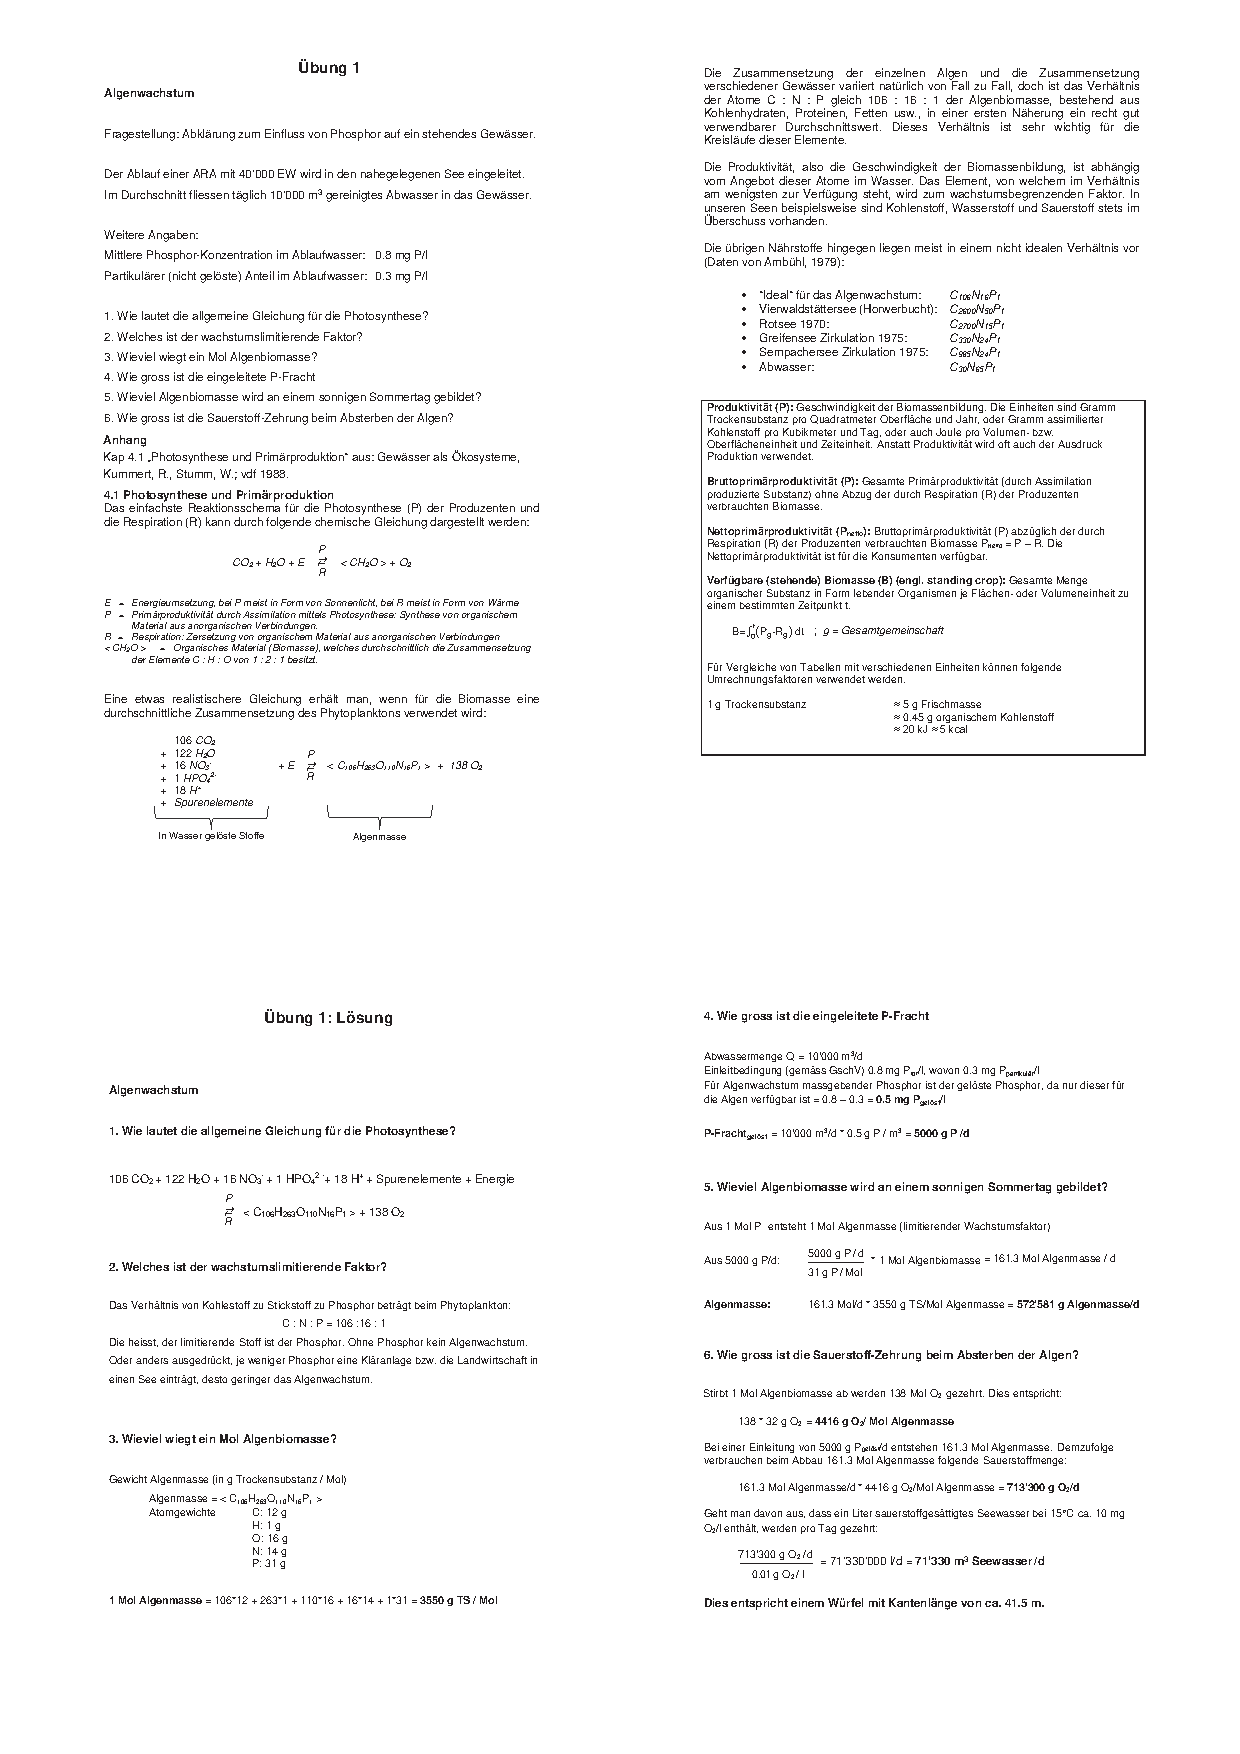
\includegraphics[width=.95\textwidth]{images/uebung1}
\end{center} 
\begin{center}
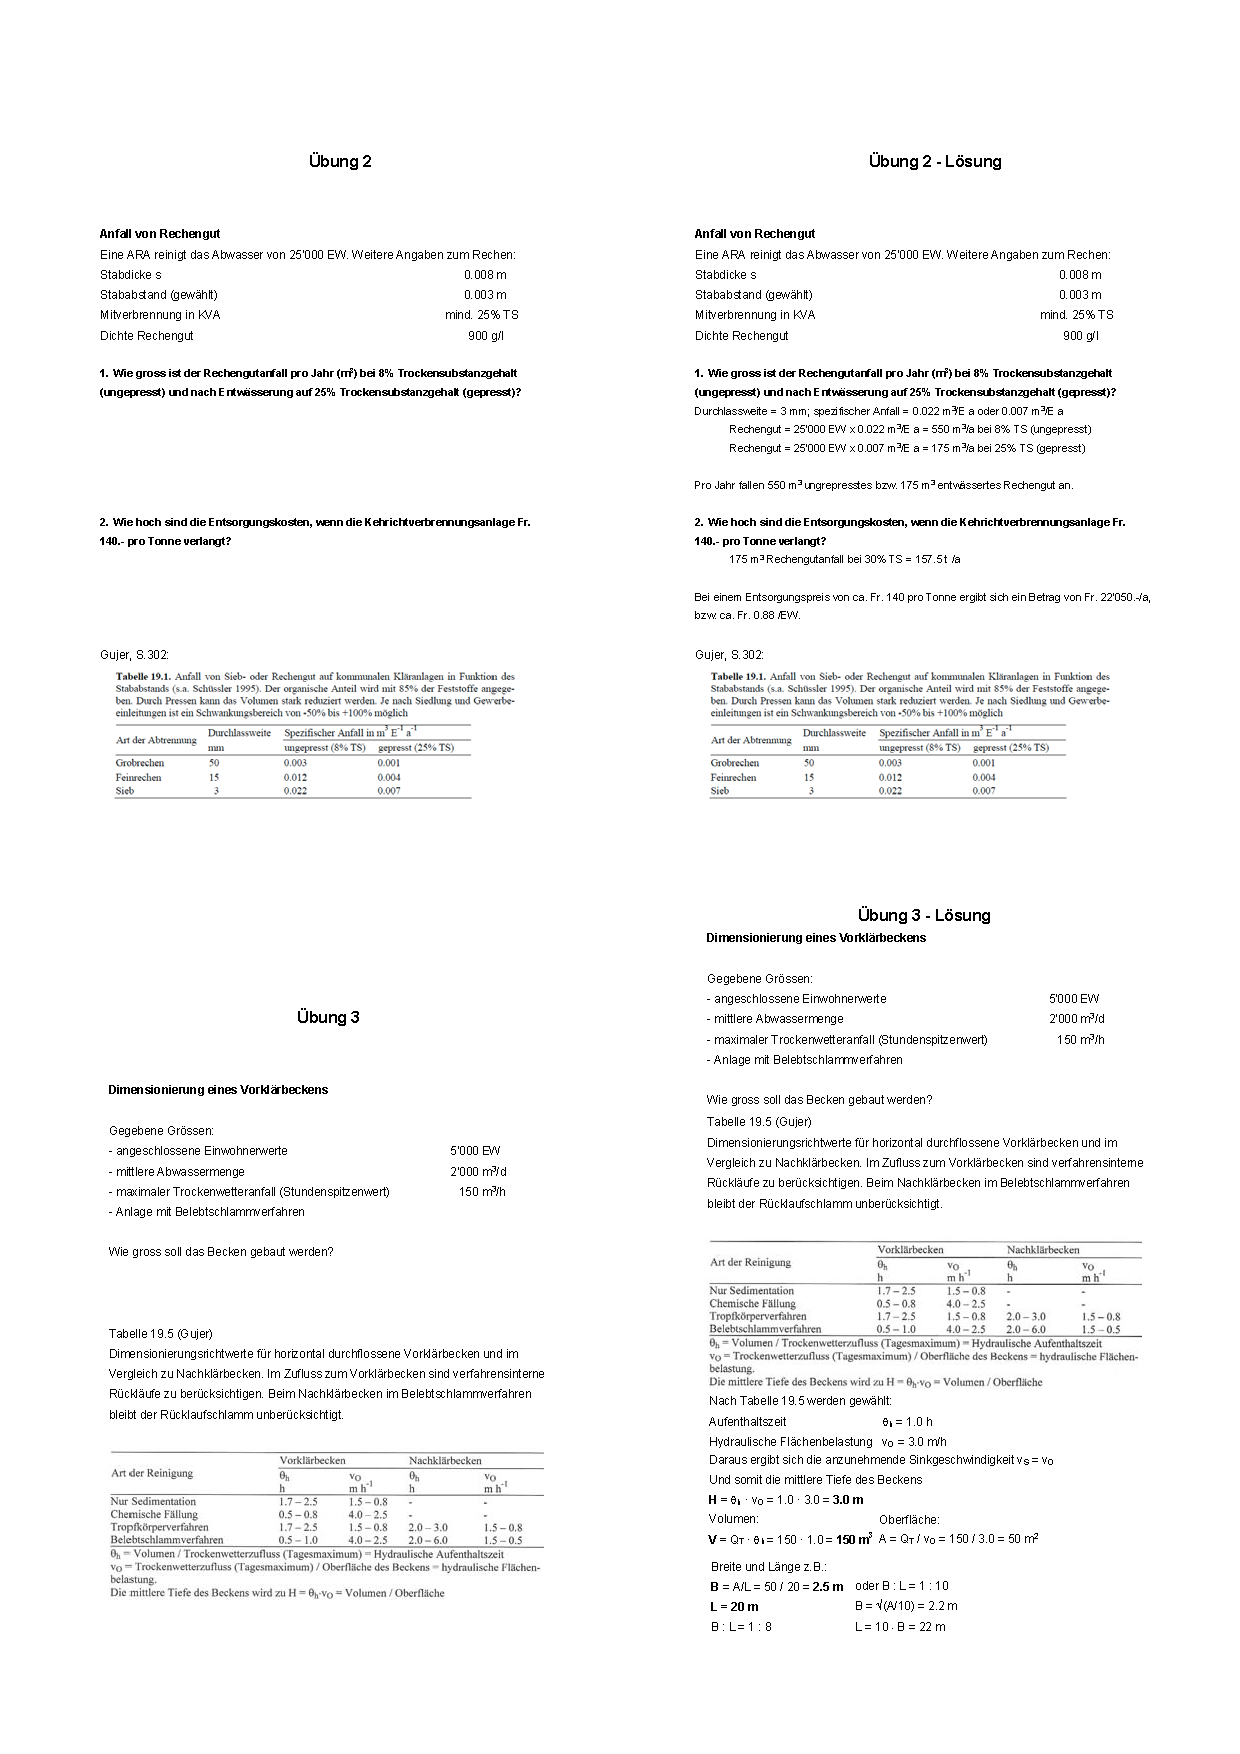
\includegraphics[width=\textwidth]{images/uebung23}
\end{center} 
\begin{center}
\includegraphics[width=\textwidth]{images/uebung4}
\end{center} 
\newpage
\section{Periodensystem der Elemente}
\begin{center}
\includegraphics[width=0.95\textwidth]{images/periodensystem}
\end{center}
\begin{small}
Quelle: Anhang zum Skript im Modul Chemie 1, HSR Hochschule für Technik
\end{small}
\clearpage
\renewcommand{\indexname}{Stichwortverzeichnis}
% Stichwortverzeichnis soll im Inhaltsverzeichnis auftauchen
\addcontentsline{toc}{section}{Stichwortverzeichnis}
% Stichwortverzeichnis endgueltig anzeigen
\printindex


\end{document}